%============================================================================
% Lizenz
%
% Das Skript ist ausschliesslich für privaten Gebrauch zu verwenden und nicht 
% zur Veröffentlichung oder kommerziellen Nutzung.
%
%============================================================================
% Shortcuts
%
% Matrix: \begin{pmatrix} \end{pmatrix}
% Linie: \vspace*{0.2cm} \\ \rule{\linewidth}{0.3mm}\vspace*{0.1cm}
% Beweisabschluss: \hfill $\Box$
% Kalligraphische Buchstaben: \mathcal{F}
% Aus Menge ausschliessen: \setminus
% Direkte Summe (Untervektorräume): \oplus 
% New line nach paragraph: {\ \\}
% Box um Text: \makebox
% Linie über Formel: \overline{x}
% Klammern unter Formel: \underbrace{w_1, ..., w_k}_{\text{Basis von } W_1}
%
%============================================================================

\documentclass[11pt,a4paper]{scrreprt}

% Basispakete
\usepackage[pdftex]{hyperref}
\usepackage[utf8]{inputenc}
\usepackage{amsmath}
\usepackage[automark]{scrpage2}
\usepackage{graphicx}
\usepackage{amssymb}
\usepackage{ifthen}
\usepackage{calc}
\usepackage{tikz}
\usetikzlibrary{matrix,calc,intersections}
\usepackage{ngerman}
\usepackage{makeidx}

% TikZ
\usetikzlibrary{automata,positioning}
\newcommand{\tikzAngleOfLine}{\tikz@AngleOfLine}
  \def\tikz@AngleOfLine(#1)(#2)#3{%
  \pgfmathanglebetweenpoints{%
    \pgfpointanchor{#1}{center}}{%
    \pgfpointanchor{#2}{center}}
  \pgfmathsetmacro{#3}{\pgfmathresult}%
  }

% Matrizen
\makeatletter
\renewcommand*\env@matrix[1][*\c@MaxMatrixCols c]{%
  \hskip -\arraycolsep
  \let\@ifnextchar\new@ifnextchar
  \array{#1}}
\makeatother

%--------------
\usepackage{thmtools, thm-restate}
\declaretheorem{satz}

% Kreis für Gleichungen
\newcommand*\mycirc[1]{%
  \begin{tikzpicture}
    \node[draw,circle,inner sep=1pt] {#1};
  \end{tikzpicture}}

% Seitenstil scrheadings verwenden
\pagestyle{scrheadings} 

% Grösse des Textbereiches in der Seite
\setlength{\textwidth}{15cm}
\setlength{\textheight}{21cm}

% Kopf- und Fusszeile, Höhe und Abstand vom Text
\setlength{\headheight}{15pt}
\setlength{\headsep}{0.8cm}

% Linker Seiteneinzug
\setlength{\oddsidemargin}{2.5cm} \addtolength{\oddsidemargin}{-1in}
\setlength{\evensidemargin}{2.5cm} \addtolength{\evensidemargin}{-1in}

% Andere Grössen ausrechnen (vertikal zentrieren)
\setlength{\footskip}{\headsep}
\addtolength{\footskip}{\headheight}
\setlength{\topmargin}{\paperheight}
\addtolength{\topmargin}{-\textheight}
\addtolength{\topmargin}{-\headheight}
\addtolength{\topmargin}{-\headsep}
\addtolength{\topmargin}{-\footskip}
\addtolength{\topmargin}{-2in}
\addtolength{\topmargin}{-0.5\topmargin}

% Sektion und Kapitel für Headmark
\automark[section]{chapter} 

% Separate Linie im Kopf
\setheadsepline{.4pt} 
% Kopf und Fußzeile löschen
\clearscrheadfoot

% linke Kopfzeile 
\ihead[\headmark]{\headmark}

% mittlere Fusszeile 
\cfoot[\pagemark]{\pagemark}

\makeindex

% Titel
\title{Lineare Algebra II}
\date{Frühjahrssemester 2012}
\author{ }

% Paket mdframed mit farbigen Rahmen
\usepackage{mdframed}
\newmdtheoremenv[linecolor=red]{lemma}{Lemma}[section]
\newmdtheoremenv[linecolor=blue]{proposition}[lemma]{Proposition}
\newmdtheoremenv[linecolor=green]{satz}[lemma]{Satz}

\newmdtheoremenv[linecolor=black]{korollar}[lemma]{Korollar}

\newcommand*\Zb[1] {\mathbb{#1}}
\newcommand*\f[1] {\textbf{#1}}

\newenvironment{amatrix}[1]{%
  \left(\begin{array}{@{}*{#1}{c}|c@{}}
}{%
  \end{array}\right)
}

\begin{document}

\maketitle
\tableofcontents
\newpage

%DATE 20.02.2012
\chapter{Vektorräume und Basen}
\paragraph{Themen}
\begin{itemize}
 \item Wiederholung der Hauptideen
 \item Geordnete Mengen und das Zornsche Lemma
 \item \f{Satz:} Jeder Vektorraum hat eine Basis
\end{itemize}

\section{Definitionen, Eigenschaften, Beispiele}
Zur Erinnerung... Ein \f{Vektorraum} $V$ über einem Körper $K$ ist eine Menge zusammen mit zwei Verknüpfungen:
\begin{itemize}
 \item +: $V \times V \rightarrow V$ (Addition)
 \item $\cdot$: $K \times V \rightarrow V$ (skalare Multiplikation)
\end{itemize}
wobei
\begin{itemize}
 \item $V$ mit $+$ ist eine abelsche Gruppe
 \item für $\alpha, \beta \in K$ und $v, w \in V$:
\begin{align}
(\alpha +_K \beta)\cdot v &= \alpha\cdot v  + \beta\cdot v \\
\alpha\cdot (v + w) &= \alpha\cdot v + \alpha\cdot w \\
(\alpha\cdot\beta) \cdot v &= \alpha\cdot(\beta\cdot v) \\
1 \cdot v &= v
\end{align}
\end{itemize}

\paragraph{Beispiele}
\begin{itemize}
 \item[(i)] Der Standardraum $K^n$ über $K$ besteht aus der Menge aller Spaltenvektoren
\begin{align}
K^n = \{ \begin{pmatrix} \alpha_1 \\ \vdots \\ \alpha_n \end{pmatrix}\}
\end{align}
mit komponentenweisen Addition und skalarer Multiplikation.
\item[(ii)] $Mat(m,n;K)$ mit Matrixaddition und skalarer Multiplikation.
\item[(iii)] $Alt(n;K)$, die Menge aller $n\times n$-Matrizen $A$ über $K$ mit $A^t = -A$ (schiefsymmetrische Matrizen)\index{Matrizen!schiefsymmetrische} ist ein Unterraum von $Mat(n;K)$.
\begin{align}
0 \in &Alt(n;K) \\
A^t = -A &, B^t = -B \\
\Rightarrow (\lambda A)^t &= \lambda A^t = -(\lambda A) \\
\Rightarrow (A+B)^t &= A^t + B^t \\
&= - A - B = - (A+B)
\end{align}
\item[(iv)] $\Zb{C}$ ist ein Vektorraum über $\Zb{R}$; auch $Mat(m,n;\Zb{C})$ (als eine Menge) über $\Zb{R}$.
\item[(v)] $Abb(M,K)$ die Menge aller Abbildungen von $M \neq \emptyset$ nach $K$ mit Verknüpfungen definiert durch:
\begin{align}
(\phi + \chi)(x) &= \phi(x) + \chi(x) \\
(\lambda \phi)(x) &= \lambda \phi(x)
\end{align}
ist ein Vektorraum über $K$.
\item[(vi)] $Abb(\Zb{R}, \Zb{R})$ hat Unterräume:
\begin{itemize}
\item $Pol\, \Zb{R} := \{\alpha_0 +\alpha_1 x + ... + \alpha_n x^n: \alpha_0, ..., \alpha_n \in \Zb{R}\}$
\item $C(\Zb{R}) := \{\phi \in Abb(\Zb{R}, \Zb{R}): \phi \text{ ist stetig}\}$
\end{itemize}
\item[(vii)] $Abb(\Zb{N}, \Zb{R})$, der Vektorraum aller reellen Folgen $\mathcal{F}$, hat Unterräume:
\begin{itemize}
\item $\mathcal{F}_b := \{a \in \mathcal{F}: a \text{ ist beschränkt}\}$
\item $\mathcal{F}_k := \{a \in \mathcal{F}: a \text{ ist konvergent}\}$
\end{itemize}
\end{itemize}
\vspace*{0.2cm}\rule{\linewidth}{0.3mm}\vspace{0.3cm}
Zur Erinnerung... Sei $E$ eine Teilmenge eines Vektorraums $V$ über $K$.
\begin{itemize}
 \item $E$ heisst \f{Erzeugendensystem}\index{Erzeugendensystem} von $V$, wenn 
\begin{align}
V &= Span\, E \\
(Span\, \emptyset &= \{0\})
\end{align}
$V$ heisst \f{endlich erzeugt}, wenn es ein endliches Erzeugendensystem von $V$ gibt.
\item $E$ heisst \f{linear unabhängig} (andernfalls linear abhängig), wenn für alle $n$ verschiedenen Elemente $v_1, ..., v_n$ von V gilt:
\begin{align}
\alpha_1 v_1 + ... \alpha_n v_n = 0  \\
\Rightarrow \alpha_1 = ... = \alpha_n = 0 \\
(\alpha_1, ..., \alpha_n \in K)
\end{align}
\item $E$ heisst eine \f{Basis} von $V$, wenn $E$ ein linear unabhängiges Erzeugendensystem ist.
\end{itemize}
\vspace*{0.2cm}\rule{\linewidth}{0.3mm}\vspace{0.3cm}
Sei nun $V$ ein \f{endlich erzeugter} Vektorraum über $K$:
\begin{itemize}
 \item Falls $V$ ein Erzeugendensystem von $n$ Elementen hat, dann sind je $n+1$ Elemente von $V$ linear abhängig\footnote{Lemma 3.3.2, lineare Algebra I}.
 \item Jede linear unabhängige Teilmenge von $V$ kann zu einer (endlichen) Basis ergänzt werden.
\end{itemize}
\paragraph{Idee} Seien $v_1, ..., v_n$ verschiedene linear unabhängige Elemente von $V$. Ist $\{v_1, ..., v_n\}$ kein Erzeugendensystem, dann gibt es 
\begin{align}
v_{n+1} \in V \setminus Span\{v_1, ..., v_n\}
\end{align}
wobei $\{v_1, ..., v_n\}$ linear unabhängig ist.

Daraus folgt, dass $V$ eine endliche Basis hat und je zwei Basen von $V$ gleich viele Elemente haben: die \f{Dimension}\index{Dimension}, $dim\, V$, von $V$\footnote{Satz 3.4.2, lineare Algebra I}.

\paragraph{Beispiele}
\begin{itemize}
 \item[(i)] Die \f{Standardbasis} von $K^n$ ist $\{e_1, ..., e_n\}$ mit
\begin{align}
e_i = \begin{pmatrix} 0 \\ \vdots \\ 0 \\ 1 \\ 0 \\ \vdots \\ 0 \end{pmatrix} \leftarrow \text{1 in der $i$-ten Zeile}
\end{align}
und $dim\, K^n = n$

\item[(ii)] Die Standardbasis von $Mat(m,n;K)$ ist 
\begin{align}
\{E_{ij}: 1 \leq i \leq m, 1 \leq j \leq n\}
\end{align}
mit $E_{ij} = (e_{kl})$ wobei
\begin{align}
e_{kl} = \left\{ \begin{matrix} 1 & k=i, l=j \\ 0 & \text{andernfalls}\end{matrix}\right.
\end{align}
$dim\, Mat(m,n;K) = mn$

\item[(iii)]
\begin{align}
Alt(3; \Zb{R}) = \{ \begin{pmatrix} 0 & \alpha & \beta \\ -\alpha & 0 & \gamma \\ -\beta & -\gamma & 0\end{pmatrix}: \alpha, \beta, \gamma \in \Zb{R} \}
\end{align}
Man beachte, dass 
\begin{align}
\begin{pmatrix} 0 & \alpha & \beta \\ -\alpha & 0 & \gamma \\ -\beta & -\gamma & 0\end{pmatrix} = \alpha(E_{12} - E_{21}) + \beta(E_{13} - E_{31}) + \gamma (E_{23}-E_{32})
\end{align}
und 
\begin{align}
\alpha(E_{12} - E_{21}) + \beta(E_{13} - E_{31}) + \gamma (E_{23}-E_{32}) = 0 \\
\Rightarrow \alpha = \beta = \gamma = 0
\end{align}
Also ist $\{E_{12}-E_{21}, E_{13}-E_{31}, E_{23}-E_{32}\}$ eine Basis von $Alt(3; \Zb{R})$ und $dim\, Alt(3;\Zb{R}) = 3$.

\item[(iv)] $\{1, i\}$ ist eine Basis von $\Zb{C}$ über $\Zb{R}$ (auch $\{1+i, 1-i\}, \{7-3i, 5+2i\}$) und $dim\, \Zb{C} = 2$. \\
$Mat(2; \Zb{C})$ \f{über} $\Zb{R}$ hat eine Basis: 
\begin{align}
\{E_{11}, E_{12}, E_{21}, E_{22}, i E_{11}, i E_{12}, i E_{21}, i E_{22}\} \text{ und} \\ dim\, Mat(2, \Zb{C}) = 8
\end{align}
\end{itemize}

\paragraph{Beobachtung}
$Pol\, \Zb{R}$ (auch $C(\Zb{R}), \mathcal{F}$, ...) ist \f{nicht} endlich erzeugt: für jedes endliche $E \subseteq Pol\, \Zb{R}$ git es $n \in N$ wobei $x^n \notin Span\, E$
\begin{align}
\{1, x, x^2, x^3, ...\}
\end{align}

\noindent \f{Frage:} Hat jeder Vektorraum eine Basis?\\
\f{Antwort:} Ja! Aber wir müssen das so genannte ``Zornsche Lemma''\index{Lemmata!Zornsches Lemma} (äquivalent zum ``Auswahlaxiom'') \f{annehmen}\footnote{Dieses ist nicht ``bewiesen''. Gemäss Gödel ist dieses widerspruchsfrei mit den Grundsätzen der bestehenden Mathematik, das Gleiche gilt aber auch für die Umkehrung des Lemmas.}.
%1.2
\section{Geordnete Mengen}
Eine \f{Halbordnung}\index{Halbordnung} (auch \f{Partialordnung} oder \f{Teilordnung}) einer Menge $X$ ist eine binäre Relation 
\begin{align}
\leq \, \subseteq R \times R
\end{align}
(man schreibt $x \leq y$ statt $(x, y) \in  \leq$)
so dass für alle $x, y, z \in X$ gilt
\begin{itemize}
\item[(i)] $x \leq x$ (Reflexivität)
\item[(ii)] $x \leq y$ und $y\leq z$ $\Rightarrow$ $x \leq z$ (Transitivität)
\item[(iii)] $x \leq y$ und $y \leq x$ $\Rightarrow x = y$ (Antisymmetrie) \\\\
\noindent $X$ mit $\leq$ heisst eine \f{halbgeordnete Menge}. Falls auch für alle $x, y \in X$ gilt:
\item[(iv)] $x \leq y$ oder $y \leq x$ heisst $\leq$ eine \f{Totalordnung}\index{Totalordnung} und $X$ mit $\leq$ eine totalgeordnete Menge.
\end{itemize}

\vspace*{0.2cm}\rule{\linewidth}{0.3mm}\vspace{0.2cm}

\paragraph{Beispiele}
\begin{itemize}
\item[(i)] Sei ``$\leq$'' die kleiner-gleich Relation: Dann sind $\Zb{N}$ mit $\leq$, $\Zb{R}$ mit $\leq$ usw. totalgeordnete Mengen.
\item[(ii)] Sei $Y$ eine Menge von Mengen. Dann gilt für alle $A, B, C \in Y$: $A \subseteq A, A \subseteq B$ und $B \subseteq C \Rightarrow A \subseteq C$. Mit $A \subseteq B$ und $B \subseteq A \Rightarrow A=B$.
Also ist $Y$ mit $\leq$ eine halbgeordnete Menge (nicht notwendigerweise totalgeordnet).
\item[(iii)] $\Zb{N}$ mit Teilbarkeit |
\begin{align}
x|y \text{ gdw } y \text{ ist teilbar durch } x 
\end{align}
ist eine halbgeordnete (nicht totalgeordnete) Menge.
\end{itemize}

\paragraph{Beobachtung}
Man kann eine endliche halbgeordnete Menge durch einen sogenanntes ``Hasse Diagramm'' darstellen.

z.B. $P(\{a, b, c\})$ mit $\subseteq$:

\begin{center}
\begin{tikzpicture}[scale=2.4, auto,swap]
\foreach \pos/\name/\disp in {{(1,3)/abc/abc}, {(0,2)/ab/ab}, {(1,2)/ac/ac}, {(2,2)/bc/bc}, {(0,1)/a/a}, {(1,1)/b/b}, {(2,1)/c/c}, {(1,0)/z/$\O$}}
\node[circle,fill=black!12,minimum size=20pt,inner sep=0pt] (\name) at \pos {$\disp$};

% Connect vertices with edges
\foreach \source/ \dest in {abc/ab, abc/ac, abc/bc, ab/a, ab/b, ac/a, ac/c, bc/b, bc/c, a/z, b/z, c/z}
\path[draw,thick,-] (\source) -- node {} (\dest);

\end{tikzpicture}
\end{center}

\newpage
Die Teiler von 36 mit \big|:
\begin{center}
\begin{tikzpicture}[scale=1.8, auto,swap]
\foreach \pos/\name/\disp in {{(2,4)/a/36}, {(1,3)/b/12}, {(3,3)/c/18}, {(0,2)/d/4}, {(2,2)/e/6}, {(4,2)/f/9}, {(1,1)/g/2}, {(3,1)/h/3}, {(2,0)/i/1}}
\node[circle,fill=black!12,minimum size=20pt,inner sep=0pt] (\name) at \pos {$\disp$};

% Connect vertices with edges
\foreach \source/ \dest in {a/b, a/c, b/d, b/e, c/e, c/f, d/g, e/g, e/h, f/h, g/i, h/i}
\path[draw,thick,-] (\source) -- node {} (\dest);

\end{tikzpicture}
\end{center}

%DATE 24.02.2012
\newpage
\noindent \textit{Vorlesung vom 24.02.2012}
\paragraph{Beispiele}
\begin{itemize}
 \item[(i)] Eine Menge $W$ von Wörtern mit der alphabetischen / lexikographischen Ordnung (Totalordnung) (``Apfel'' $<$ ``Bär'' $<$ ``braun'' $<$ ...)
 \item[(ii)] Die Unterräume eines Vektorraums mit $\subseteq$
 \item[(iii)]
   \begin{center}
   \begin{tikzpicture}[scale=1.8, auto,swap]
   \foreach \pos/\name/\disp in {{(1,0)/a/a}, {(0,1)/b/b}, {(2,1)/c/c}, {(1,2)/d/d}}
   \node[circle,fill=black!12,minimum size=20pt,inner sep=0pt] (\name) at \pos {$\disp$};
   \foreach \source/ \dest in {a/b, a/c, b/d, c/d} % Connect vertices with edges
   \path[draw,thick,-] (\source) -- node {} (\dest);
   \end{tikzpicture}
   \end{center}
\begin{align}
X = \{a, b, c, d\}\\
\subseteq = \{(a, a), (a, b), (a, c), (a, d), (b, b), (b, c), (b, d), (c, c), (c, d), (d, d)\}
\end{align}
\end{itemize}

Sei $X$ mit $\subseteq$ eine halbgeordnete Menge.
\begin{itemize}
 \item $a \in X$ ist eine \f{obere Schranke}\index{Schranke} für $Y \subseteq X$ wenn $b \leq a\, \forall\, b \in Y$
 \item $a \in X$ ist ein \f{maximales Element}\index{maximales Element}, wenn es kein $b \in X$ mit $b \neq a$ und $a \leq b$ gibt
\end{itemize}

\paragraph{Beispiel}
\begin{itemize}
\item $P(\{a, b, c\}) \setminus \{a, b, c\}, \subseteq$:
   \begin{center}
   \begin{tikzpicture}[scale=1.8, auto,swap]
   \foreach \pos/\name/\disp in {{(1,0)/a/\emptyset}, {(0,1)/b/\{a\}}, {(1,1)/c/\{b\}}, {(2,1)/d/\{c\}}, {(0,2)/e/\{a, b\}}, {(1,2)/f/\{a, c\}}, {(2,2)/g/\{b, c\}}}
   \node[circle,fill=black!12,minimum size=20pt,inner sep=0pt] (\name) at \pos {$\disp$};
   \foreach \source/ \dest in {a/b, a/c, a/d, b/e, b/f, c/e, c/g, d/f, d/g} % Connect vertices with edges
   \path[draw,thick,-] (\source) -- node {} (\dest);
   \end{tikzpicture}
   \end{center}
$\{a, b\}$, $\{a, c\}$ und $\{b, c\}$ sind maximale Elemente. 
\item \f{Untere Schranken} und \f{minimale Elemente} sind analog definiert. $(X, \subseteq)$ heisst \f{induktiv}\index{induktiv}, wenn jede totalgeordnete Teilmenge $Y$ von $X$ eine obere Schranke in $X$ hat. (Ist $X$ \f{endlich}, dann ist $(X, \subseteq)$ immer induktiv. Aber z.B. $(\Zb{N}, \subseteq)$ ist nicht induktiv.)
\end{itemize}

\paragraph{Das Zornsche Lemma} {\ \\}
Eine induktive halbgeordnete Menge hat ein maximales Element.

\begin{satz} % 1.2.1
Jeder Vektorraum $V$ hat eine Basis.
\end{satz}

\paragraph{Beweis}
Sei $X$ die Menge aller linear unabhängiger Teilmengen von $V$. Wir zeigen, dass $(X, \subseteq)$ \f{induktiv} ist. Sei $Y$ eine totalgeordnete Menge von $X$. Wir behaupten, dass
\begin{align}
 B = \bigcup _{A \in Y} A
\end{align}
linear unabhängig ist und deshalb eine obere Schranke von $Y$ in $X$. Man betrachtet $\alpha_1 v_1 + ... + \alpha_n v_n = 0$ mit $\alpha_1, ..., \alpha_n \in K$ und $v_1, ..., v_n \in B$ d.h. für $i=1, ..., n: v_i \in A_i$ für ein $A_i \in Y$. Man darf auch annehmen: $A_1 \subseteq A_2 \subseteq ... \subseteq A_n$, da $Y$ totalgeordnet ist. Also ist $v_i \in A_n$ für $i = 1, ..., n$ und weil $A_n$ linear unabhängig ist, folgt $\alpha_1 = ... = \alpha_n = 0$, d.h. $B$ ist linear unabhängig.
Nach dem Zornschen Lemma erhält man ein maximales Element $M$ von $X$. Nach Definition von $X$ ist $M$ linear unabhängig.\\\\
Ist $M$ ein Erzeugendensystem von $V$?\\
Sei $v \in V$. Ist $v \notin Span\, M$, dann ist $M \cup \{v\}$ linear unabhängig. Dies steht im Widerspruch zur Maximalität von $M$. Also $Span\, M = V$ und $M$ ist eine Basis von $V$. \hfill $\Box$

\paragraph{Bemerkung}
Das Zornsche Lemma ist äquivalent zu:
\begin{itemize}
\item dem \f{Auswahlaxiom}: ``Für jede Menge von nichtleeren Mengen $X$ gibt es eine Funktion
\begin{align}
f: X \rightarrow \cup X
\end{align}
wobei $Y \in X \Rightarrow f(Y) \in Y$.''\\
Beispiel: $X = \{\{a\}, \{b, c\}, \{a, b, c\}, \Zb{N}\}$\\
$f(\{a\}) = a, f(\{a, b, c\},) = b, f(\{b, c\}) = b, f(\Zb{N}) = 73$
\item dem \f{Wohlordnungssatz}: ``Für jede Menge $X$ gibt es eine 'Wohlordnung' $\subseteq$, d.h. eine Totalordnung von $X$, wobei jede nichtleere Teilmenge von $X$ ein kleinstes Element bezüglich $\subseteq$ hat.''\\
Beispiel: $(\Zb{N}, \leq)$ ist eine wohlgeordnete Menge, aber nicht $(\Zb{Z}, \leq)$ (kein kleinstes Element) oder $(\Zb{R}, \leq)$: $0 < 1 < -1 < 2 < -2 < ...$ (hat $\Zb{R}$ eine Wohlordnung?)
\end{itemize}

\chapter{Eigenvektoren} % 2
\section{Homomorphismen und Matrizen} % 2.1
Zur Erinnerung: Seien $V$ und $W$ Vektorräume über demselben Körper K. Eine Abbildung $f: V \rightarrow W$ heisst \f{Homomorphismus}\index{Homomorphismus} (lineare Abbildung), wenn
\begin{itemize}
\item[(1)] $f(x + y) = f(x) + f(y)$ $x, y \in V$
\item[(2)] $f(\alpha x) = \alpha f(x)$ $x \in V, \alpha \in K$
\end{itemize}
Daraus folgt (durch Induktion):
\begin{align}
f \left( \sum_{i=1}^{n} \alpha_i v_i\right) = \sum_{i=1}^{n} \alpha_i f(v_i)
\end{align}
Man definiert auch: Kern $f := \{v \in V: f(v) = 0\}$, Bild $f:= \{f(v): v \in V\}$ und zeigt\footnote{Lineare Algebra 1, Satz 4.2.5}, dass wenn $V$ endlich erzeugt ist, gilt: 
\begin{align}
dim\, Kern\, f + dim\, Bild\, f = dim\, V
\end{align}

\paragraph{Beispiele}
\begin{itemize}
\item[(i)] Sei $A \in Mat(m,n;K)$. Dann ist $h_A: K^n \rightarrow K^m, x \mapsto Ax$ ein Homomorphismus
\begin{align}
h_A(\alpha x + \beta y) &= A (\alpha x + \beta y) \\
&= \alpha Ax + \beta A y \\
&= \alpha h_A (x) + \beta h_A (y)
\end{align}
\item[(ii)] Der \f{transponierte Operator} $f: Mat(m,n;K) \rightarrow Mat(m,n;K), A \mapsto A^T$ ist ein Homomorphismus, eigentlich ein \f{Isomorphismus}.
\item[(iii)] Die Abbildung 
\begin{align}
f: \Zb{C}[0,1] \rightarrow \Zb{R}\;\; (\Zb{C}[0,1] &= \{\phi \in Abb([0,1], \Zb{R}), \phi \text{ stetig.}\})\\
&\phi \mapsto \int_{0}^{1} \phi(x) dx\\
\int_{0}^{1}(\alpha \phi + \beta \chi)(x) dx &= \alpha \int_{0}^{1} \phi(x) dx + \beta \int_{0}^{1} \chi(x) dx
\end{align}
\end{itemize}
Man kann Homomorphismen zwischen endlich erzeugten Vektorräumen \f{mit Matrizen darstellen}, z.B.
\begin{align}
f: \Zb{R}^3 \rightarrow \Zb{R}^2, \begin{pmatrix} \alpha \\ \beta \\ \gamma \end{pmatrix} \mapsto \begin{pmatrix} \alpha + 2 \beta \\ -\alpha + \beta - 3\gamma \end{pmatrix}
\end{align}
ist bezüglich der Standardbasen durch Linksmultiplikation mit der Matrix 
\begin{align}
\begin{pmatrix} 1 & 2 & 0 \\ -1 & 1 & -3 \end{pmatrix}
\end{align}
gegeben.\\
Beachten Sie, dass 
\begin{align}
f(\begin{pmatrix} 1 \\ 0 \\ 0 \end{pmatrix}) = \begin{pmatrix} 1 \\ -1 \end{pmatrix} = 1 \begin{pmatrix} 1 \\ 0 \end{pmatrix} + (-1) \begin{pmatrix} 0 \\ 1 \end{pmatrix} \\
f(\begin{pmatrix} 0 \\ 1 \\ 0 \end{pmatrix}) = \begin{pmatrix} 2 \\ 1 \end{pmatrix} = 2 \begin{pmatrix} 1 \\ 0 \end{pmatrix} + 1 \begin{pmatrix} 0 \\ 1 \end{pmatrix} \\
f(\begin{pmatrix} 0 \\ 0 \\ 1 \end{pmatrix}) = \begin{pmatrix} 0 \\ -3 \end{pmatrix} = 0 \begin{pmatrix} 1 \\ 0 \end{pmatrix} + (-3) \begin{pmatrix} 0 \\ 1 \end{pmatrix}
\end{align}
Für einen Homomorphismus $f: K^n \rightarrow K^m$ betrachtet man $f(e_j) = \sum_{i=1}^{m} \alpha_{ij} e_i, j=1...n$ und erhält $f(x) = Ax$ mit $A = (\alpha_{ij})$.\\\\
Sei nun $V$ ein endlich erzeugter Vektorraum über $K$ und $B = (v_1, ..., v_n)$ eine geordnete Basis von $V$.
Man definiert 
\begin{align}
q_B: V \rightarrow K^n \\
v \mapsto \begin{pmatrix} \alpha_1 \\ \vdots \\ \alpha_n \end{pmatrix}
\end{align}
mit $v = (\alpha_1 v_1 + ... + \alpha_n v_n)$ ein Isomorphismus von $V$ in $K^n$.
Sei auch $W$ ein endlich erzeugter Vektorraum über $K$ und $C = (w_1, ..., w_m)$ eine geordnete Basis von $W$.
Für ein Homomorphismus $f: V \rightarrow W$ betrachtet man 
\begin{align}
f(v_j) = \sum_{i = 1}^{m} \alpha_{ij} w_i, j=1...n \\
\text{d.h. } q_C (f(v_j)) = \begin{pmatrix} \alpha_{ij} \\ \vdots \\ \alpha_{mj} \end{pmatrix}
\end{align}
und erhält
\begin{align}
\mathcal{M}_{C}^{B} (f) = (\alpha_{ij}) = (q_C(f(v_1))), ..., q_C(f(v_n))
\end{align}
die \f{Matrix von $f$ bezüglich der Basen $B$ und $C$}.
\begin{center}
\begin{tikzpicture}
\matrix (m) [matrix of math nodes,row sep=3em,column sep=4em,minimum width=2em] {
V & W \\
K^n & K^m \\};
\path[-stealth]
(m-1-1) edge [<->] node [right] {$q_B$} node [left] {$q_{B}^{-1}$} 
(m-2-1) edge node [above] {$f$} 
(m-1-2)
(m-2-1.east|-m-2-2) edge node [above] {$\hat{f}$} 
(m-2-2)
(m-1-2) edge node [right] {$q_C$} 
(m-2-2)
(m-2-1);
\end{tikzpicture}
\end{center}
\begin{align}
\hat{f} = q_C \circ f \circ q_{B}^{-1}
\end{align}
Man beobachtet:
\begin{align}
\mathcal{M}_{C}^{B} (f) (q_B(v)) = (q_C \circ f \circ q_{B}^{-1})(q_{B}(v)) = q_C(f(v))
\end{align}
Beispiel: $\Zb{C}$ über $\Zb{R}$ hat eine geordnete Basis $B = (1+i, 1-i)$. $P_2 = \{\alpha + \beta x + \gamma x^2: \alpha, \beta, \gamma \in \Zb{R}\}$ hat eine geordnete Basis $C = (1+x^2, x, 2x^2 + 1)$. \\
Wir betrachten $f: \Zb{C} \rightarrow P_2, a + b i \mapsto a + (a+b)x + bx^2$
\begin{align}
f(1+i) &= 1 + 2x + x^2 \\
&= 1 (1+x^2) + 2(x) + 0(2x^2+1) \\
f(1-i) &= 1-x^2 \\
&= 3(1+x^2) + 0(x) + (-2)(2x^2 + 1)
\end{align}
Also
\begin{align}
q_C(f(1+i)) = \begin{pmatrix} 1 \\ 2 \\ 0 \end{pmatrix} \\
q_C(f(1-i)) = \begin{pmatrix} 3 \\ 0 \\ -2 \end{pmatrix} \text{ und } \mathcal{M}_{C}^{B}(f) = \begin{pmatrix} 1 & 3 \\ 2 & 0 \\ 0 & -2 \end{pmatrix}
\end{align}
Zum Beispiel:
\begin{align}
q_B(5+i) = \begin{pmatrix} 3 \\ 2 \end{pmatrix} \\
q_C(f(5+i)) = \begin{pmatrix} 1 & 3 \\ 2 & 0 \\ 0 & -2 \end{pmatrix} \begin{pmatrix} 3 \\ 2 \end{pmatrix} = \begin{pmatrix} 9 \\ 6 \\ -4 \end{pmatrix}\\
f(5+i) = 5 + 6x + x^2 = 9(1+x^2) + 6(x) + (-4)(2x^2+1)
\end{align}

%DATE 27.02.2012
\newpage
\noindent \textit{Vorlesung vom 27.02.2012} \\
\f{2.1 Homomorphismen und Matrizen} \\\\ % 2.1
Sei $V$ ein Vektorraum über $K$ und $B = (b_1, ..., b_n)$ eine (geordnete) Basis von $V$.\\
\f{Frage:} Wie beschreibt/findet man alle anderen Basen von $V$? \\\\
Sei $c_1, ..., c_n$ verschiedene Elemente von $V$ mit
\begin{align}
c_i = \sum_{j=1}^{n} \alpha_{ji} b_j \,\,(i = 1...n) \\
\text{d.h. } q_B (c_i) = \begin{pmatrix} \alpha_{1i} \\ \vdots \\ \alpha_{ni} \end{pmatrix}
\end{align}
Dann ist $C = (c_1, ..., c_n)$ eine \f{Basis} 
\begin{itemize}
 \item gdw $c_1, ..., c_n$ linear unabhängig sind
 \item gdw $A = (\alpha_{ij}) = (q_B(c_1) ... q_B (c_n)) \in GL(n;K)$, d.h. $A$ ist \f{invertierbar}\footnote{Lineare Algebra 1, Lemma 5.4.1}
\end{itemize}
$A$ ist die \f{Übergangsmatrix} $T_{B}^{C}$ von $C$ nach $B$, und $A^{-1}$ ist die Übergangsmatrix von $B$ nach $C$.

Man beobachtet, dass für $i = 1...n$ 
\begin{align}
q_B (c_i) = 
\begin{pmatrix}
\alpha_{1i} \\ \vdots \\ \alpha_{ni}
\end{pmatrix}
=
\begin{pmatrix}
\alpha_{1i} & \cdots & \cdots & \cdots & \alpha_{1n} \\ 
\vdots & \ddots &  & & \vdots \\ 
\vdots & & \ddots & & \vdots \\ 
\vdots & & & \ddots & \vdots \\ 
\alpha_{ni} & \cdots & \cdots & \cdots & \alpha_{nn}
\end{pmatrix}
\begin{pmatrix}
0 \\ \vdots \\ 0 \\ 1 \\ 0 \\ \vdots \\ 0
\end{pmatrix}
\leftarrow \text{ $i$-te Stelle} \\
= A q_C (c_i)
\end{align}
und deshalb, für alle $v \in V$
\begin{align}
q_B (v) = A q_C(v), q_c(v) = A^{-1} q_B (v)
\end{align}
Beispiel: $B = (1 + x, 1 - x)$ ist eine Basis von $P_1 = \{\alpha x + \beta: \alpha, \beta \in \Zb{R}\}$
\begin{align}
A =
\begin{pmatrix}
3 & 2 \\ 2 & -1
\end{pmatrix}
\in GL(2; \Zb{R})
\end{align}
Also ist $(c_1, c_2)$ eine Basis von $P_1$ mit
\begin{align}
q_B (c_1) = \begin{pmatrix} 3 \\ 2 \end{pmatrix}, q_B (c_2) = \begin{pmatrix} 2 \\ -1 \end{pmatrix} \\
c_1 = 3(1+x) + 2(1-x) = x+ 5 \\
c_2 = 2(1 + x) - 1 (1-x) = 3x + 1
\end{align}
\vspace*{0.2cm}\rule{\linewidth}{0.3mm}\vspace{0.2cm}
Betrachten Sie nun endlich erzeugte Vektorräume
\begin{itemize}
 \item $V$ mit Basis $B$
 \item $W$ mit Basis $C$
\end{itemize}
und einen Homomorphismus
\begin{align}
f: V \rightarrow W
\end{align}
Dann gilt für \f{andere Basen} $B'$ von $V$ und $C'$ von $W$:

\begin{align}
q_{B}' &= h_{T_{B'}^{B}} \circ q_{B} \\
q_{C}' &= h_{T_{C'}^{C}} \circ q_{C} \\
h_{\mathcal{M}_{C}^{B}(f)} &= q_{C} \circ f \circ q_{B}^{-1} \\
\fbox{$h_{\mathcal{M}_{C'}^{B'}(f)}$} &= q_{C'} \circ f \circ (q_{B'})^{-1}
\end{align}

\begin{center}
\begin{tikzpicture}
\matrix (m) [matrix of math nodes,row sep=3em,column sep=4em,minimum width=2em] {
V & W \\
K^n & K^m \\};
\path[-stealth]
(m-1-1) edge [<->] node [right] {$q_B$} node [left] {$q_{B}^{-1}$} 
(m-2-1) edge node [above] {$f$} 
(m-1-2)
(m-2-1.east|-m-2-2) edge node [above] {$\hat{f}$} node [below] {\footnotesize $q_C \circ f \circ q_B^{-1}$} 
(m-2-2)
(m-1-2) edge node [right] {$q_C$} 
(m-2-2)
(m-2-1);
\end{tikzpicture}
\end{center}
\normalsize

\begin{align}
&= (h_{T_{C'}^{C}} \circ q_C) \circ f \circ (h_{T_{B'}^{B}} \circ q_B)^{-1} \\
&= h_{T_{C'}^{C}} \circ (q_C \circ f \circ q_B^{-1}) \circ (h_{T_{B'}^{B}})^{-1} \\
&= h_{T_{C'}^{C}} \circ h_{\mathcal{M}_{C}^{B}(f)} \circ (h_{T_{B'}^{B}})^{-1} \\
\text{und } \mathcal{M}_{C'}^{B'}(f) &= T_{C'}^{C}, \mathcal{M}_{C}^{B}(f) (T_{B'}^{B})^{-1}
\end{align}
Deshalb ist $A$ die Matrix von $f$ bezüglich anderen Basen \f{gdw} 
\begin{align}
A = Q \mathcal{M}_{C}^{B} (f) P^{-1}
\end{align}
für \f{beliebige} invertierbare Matrizen $P$ und $Q$.\\\\
\f{Frage:} Wie findet man die 'beste Matrix-Darstellung' von $f$? \\
\f{Antwort:} Man verwendet elementare Spalten- und Zeilenumformungen .

\paragraph{Beispiel}
$\Zb{R}^3$ mit Basis 
\begin{align}
B = (\begin{pmatrix}1 \\ 0 \\ 0\end{pmatrix}, \begin{pmatrix} 0 \\ 1 \\ 0\end{pmatrix}, \begin{pmatrix} 0 \\ 0 \\ 1\end{pmatrix})
\end{align}
$\Zb{C}$ über $\Zb{R}$ mit Basis $C = (1, i)$.
\begin{align}
f : \Zb{R}^3 \rightarrow \Zb{C}, \begin{pmatrix} \alpha \\ \beta \\ \gamma \end{pmatrix} \mapsto (\alpha + \beta) + (\beta + \gamma)i \\
\mathcal{M}_{C}^{B}(f) = \begin{pmatrix}1 & 1 & 0 \\ 0 & 1 & 1\end{pmatrix}
\end{align}
Wir suchen eine Darstellung:
\begin{align}
Q \mathcal{M}_{C}^{B} (f) P^{-1} = \begin{pmatrix}1 & 1 & 0 \\ 0 & 1 & 1\end{pmatrix} \\
\begin{pmatrix} 1 & 1 & 0 \\ 0 & 1 & 1 \end{pmatrix} Z_1 \rightarrow Z_1 - Z_2 \longrightarrow 
\begin{pmatrix}1 & 0 & -1 \\ 0 & 1 & 1\end{pmatrix} \\
S_3 \rightarrow S_3 + S_1 \longrightarrow \begin{pmatrix}1 & 0 & 0 \\ 0 & 1 & 1\end{pmatrix} 
S_3 \rightarrow S_3 - S_2 \longrightarrow \begin{pmatrix}1 & 0 & 0 \\ 0 & 1 & 0\end{pmatrix} \\
Q = \begin{pmatrix}1 & -1 \\ 0 & 1 \end{pmatrix} (= T_{C'}^{C}), Q^{-1} = \begin{pmatrix}1 & 1 \\ 0 & 1 \end{pmatrix} \\
P = \begin{pmatrix}1 & 0 & 1 \\ 0 & 1 & 0 \\ 0 & 0 & 1 \end{pmatrix} \begin{pmatrix}1 & 0 & 0 \\ 0 & 1 & -1 \\ 0 & 0 & 1 \end{pmatrix} = \begin{pmatrix}1 & 0 & 1 \\ 0 & 1 & -1 \\ 0 & 0 & 1 \end{pmatrix} (= (T_{B'}^{B})^{-1} = T_{B}^{B'})
\end{align}
Wir definieren:
\begin{align}
B' = (\begin{pmatrix}1 \\ 0 \\ 0\end{pmatrix}, \begin{pmatrix}0 \\ 1 \\ 0\end{pmatrix}, \begin{pmatrix}1 \\ -1 \\ 1\end{pmatrix}) \\
C' = (1, 1+i)
\end{align}
und beobachten, dass
\begin{align}
f(\begin{pmatrix}1 \\ 0 \\ 0\end{pmatrix}) = 1(1) + 0(1+i) = 1 \\
f(\begin{pmatrix}0 \\ 1 \\ 0\end{pmatrix}) = 0(1) + 1(1+i) = 1 + i\\
f(\begin{pmatrix}1 \\ -1 \\ 1\end{pmatrix}) = 0(1) + 0(1+i) = 0\\
\text{d.h. } \mathcal{M}_{C'}^{B'} (f) = \begin{pmatrix} 1 & 0 & 0 \\ 0 & 1 & 0 \end{pmatrix}
\end{align}

\paragraph{Bemerkung}
\begin{itemize}
\item[(a)] Zu jeder $A \in Mat(m,n;K)$ gibt es Produkte $Q \in GL(n;K)$ und $P^{-1} \in GL(n;K)$ von Elementarmatrizen mit
\begin{align}
Q A P^{-1} = \begin{pmatrix} E^{(r)} & 0 \\ 0 & 0\end{pmatrix}, r = \text{ Rang } A
\end{align}
\footnote{Lineare Algebra 1, Satz 5.3.9}

\item[(b)] Sei $f: V \rightarrow W$ ein Homomorphismus zwischen den endlich erzeugten Vektorräumen $V$ und $W$. Man kann Basen $B$ und $C$ finden, so dass
\begin{align}
\mathcal{M}_{C}^{B}(f) = \begin{pmatrix} E^{(r)} & 0 \\ 0 & 0\end{pmatrix}, r = \text{ Rang } f.
\end{align}
\end{itemize}

\section{Endomorphismen und Eigenvektoren} %2.2
Sei $V$ ein endlich erzeugter Vektorraum. Wir betrachten nun \f{Endomorphismen}\index{Endomorphismen}
\begin{align}
f: V \rightarrow  V
\end{align}
und suchen Matrixdarstellungen bezüglich \f{einer einzigen Basis} $B_j$ d.h.
\begin{align}
\mathcal{M}_{B} (f) := \mathcal{M}_{B}^{B} (f)
\end{align}

\paragraph{Beobachtung}
Sei $A \in Mat(n;K)$ die Matrixdarstellung von $f: V \rightarrow V$ bezüglich einer Basis $B$ von $V$, d.h. $A = \mathcal{M}_{B} (f)$. Dann ist $A' \in Mat(n;K)$ die Matrixdarstellung von $f$ bezüglich einer anderen Basis gdw
\begin{align}
A' = P A P^{-1}
\end{align}
für eine beliebige invertierbare Matrix $P \in GL(n;K)$
\vspace*{0.2cm} \\ \rule{\linewidth}{0.3mm}\vspace*{0.1cm}
\paragraph{Anmerkung} Man sucht $P \in GL(n;K)$ so dass $P A P^{-1}$ 'einfach' - vielleicht diagonal - ist. Aber wir haben jetzt nur noch eine Basis und damit auch nur eine Matrix $P$ zur Verfügung. \\
\footnotesize Man probiert vielleicht Elementarmatrizen $P_1, ..., P_k$ zu finden mit $P_1, ..., P_k = P_1$.
\begin{align}
P A P^{-1} = P_1, ..., P_k A P_{k}^{-1}, ..., P_{1}^{-1}
\end{align}
\normalsize
\vspace*{0.2cm} \\ \rule{\linewidth}{0.3mm}\vspace*{0.1cm}
Sei $f: V \rightarrow V$ ein Endomorphismus eines Vektorraums. Ein Unterraum $W$ von $V$ heisst \f{f-invariant}, wenn
\begin{align}
f(W) \subseteq W
\end{align}
In diesem Fal ist $f: W \rightarrow W$ die \f{Beschränkung von $f$ auf $W$}, auch ein Endomorphismus.

\paragraph{Beispiel}
\begin{align}
f: \Zb{R}^3 \rightarrow \Zb{R}^3 \\
\begin{pmatrix} \alpha \\ \beta \\ \gamma\end{pmatrix} \mapsto \begin{pmatrix} 2\alpha - \beta - \gamma \\ \alpha + \beta \\ \alpha + \gamma \end{pmatrix} \\
W = Span\{\begin{pmatrix} 1 \\ 0 \\ 0\end{pmatrix}, \begin{pmatrix} 1 \\ 1 \\ 1\end{pmatrix}\} \\
f(\begin{pmatrix} 1 \\ 0 \\ 0\end{pmatrix}) = \begin{pmatrix} 2 \\ 1 \\ 1\end{pmatrix} = 1 \begin{pmatrix} 1 \\ 0 \\ 0\end{pmatrix} + 1 \begin{pmatrix} 1 \\ 1 \\ 1 \end{pmatrix} \in W \\
f(\begin{pmatrix} 1 \\ 1 \\ 1\end{pmatrix}) = \begin{pmatrix} 0 \\ 2 \\ 2\end{pmatrix} = -2 \begin{pmatrix} 1 \\ 0 \\ 0\end{pmatrix} + 2 \begin{pmatrix} 1 \\ 1 \\ 1 \end{pmatrix}
\end{align}
Also ist $f(W) \subseteq W$ und $W$ ist f-invariant\index{invariant}.
\vspace*{0.2cm} \\ \rule{\linewidth}{0.3mm}\vspace*{0.1cm}
Sei $f: V \rightarrow V$ ein Endomorphismus eines Vektorraums und 
\begin{align}
(w_1, ..., w_k)
\end{align}
eine Basis eines f-invarianten Unterraums $W$ von $V$. Sei nun
\begin{align}
B = (w_1, ..., w_k, v_1, ..., v_{n-k})
\end{align}
eine Basis von $V$. Dann hat $\mathcal{M}_{B} (f)$ die Form
\begin{align}
\begin{pmatrix} A_1 & D \\ 0 & A_2\end{pmatrix}
\end{align}
wobei $A \in Mat(k;K)$ die Matrixdarstellung von $f: W \rightarrow W$ bezüglich $(w_1, ..., w_k)$ ist.
\paragraph{Beispiel} (siehe oben) \\
$\Zb{R}^3$ hat eine Basis:
\begin{align}
(\begin{pmatrix} 1 \\ 0 \\ 0 \end{pmatrix}, \begin{pmatrix} 1 \\ 1 \\ 1 \end{pmatrix}, \begin{pmatrix} 0 \\ 0 \\ 1 \end{pmatrix}) \text{ und } \mathcal{M}_{B} (f) = \begin{pmatrix} 1 & -2 & -1 \\ 1 & 2 & 0 \\ 1 & 0 & 1\end{pmatrix}
\end{align}
Wenn $V = W_1 \oplus W_2$ ($V = W_1 + W_2$ und $W_1 \cap W_2 = \{0\}$) und $W_1, W_2$ f-invariante Unterräume sind, erhält man eine Basis von $V$:
\begin{align}
B = (\underbrace{w_1, ..., w_k}_{\text{Basis von } W_1}, \underbrace{v_1, ..., v_{n-k}}_{\text{Basis von } W_2})
\end{align}
und $\mathcal{M}_{B} (f)$ hat die Form
\begin{align}
\begin{pmatrix} A_1 & 0 \\ 0 & A_2\end{pmatrix}
\end{align}

\paragraph{Idee} Für einen Endomorphismus $f: V \rightarrow V$ suchen wir \f{1-dimensionale f-invariante Unterräume}.
Sei $f: V \rightarrow V$ ein Endomorphismus eines Vektorraums $V$ über $K$. Wenn
\begin{align}
f(v) = \alpha v \text{ mit }0 \neq v \in V, \alpha \in K
\end{align}
heisst $v$ ein \f{Eigenvektor} \index{Eigenvektor} und ein \f{Eigenwert} (der zum Eigenvektor $v$ gehört) von $f$.

%DATE 05.03.2012
\newpage
\noindent \textit{Vorlesung vom 05.03.2012} \\
\noindent \f{2.2 Endomorphismen und Eigenvektoren} \\
\paragraph{Beispiel}
Betrachte den \f{Endomorphismus}
\begin{align}
f_{\theta}: \Zb{R}^2 \rightarrow \Zb{R}^2, \begin{pmatrix} r \cdot cos (\alpha) \\  r \cdot sin (\alpha) \end{pmatrix} \mapsto \begin{pmatrix} r \cdot cos (\alpha + \theta) \\  r \cdot sin (\alpha + \theta) \end{pmatrix} \\
\theta \in [0, 2\pi]
\end{align}
eine \f{Drehung} der Ebene um einen Winkel $\theta$.
\begin{center}
\begin{tikzpicture}[scale=2.7,cap=round]
  % Local definitions
  \def\costhirty{0.8660256}

  % Colors
  \colorlet{anglecolor}{green!50!black}
  \colorlet{sincolor}{red}
  \colorlet{tancolor}{orange!80!black}
  \colorlet{coscolor}{blue}

  % Styles
  \tikzstyle{axes}=[]
  \tikzstyle{important line}=[very thick]
  \tikzstyle{information text}=[rounded corners,fill=red!10,inner sep=1ex]

  % The graphic
  \draw[style=help lines,step=0.5cm] (-1.4,-0.4) grid (1.4,1.4);

  \begin{scope}[style=axes]
    \draw[->] (-1.5,0) -- (1.5,0) node[right] {$x$};
    \draw[->] (0,-0.5) -- (0,1.5) node[above] {$y$};
  \end{scope}

  \draw[fill=green!30] (0,0) -- (right:.5cm) arc (0:30:.5cm);
  \draw(15:0.3cm) node {$\alpha$};

  \draw[->] (0,0) -- (1,0.58) node[right] {$\begin{pmatrix} r \cdot cos \, \alpha \\ r \cdot sin \, \alpha \end{pmatrix} $};

  \draw[fill=blue!50] (0,0) -- (30:.5cm) arc (30:60:.5cm);
  \draw(45:0.3cm) node {$\theta$};

  \draw[->] (0,0) -- (0.58,1) node[right] {$\begin{pmatrix} r \cdot cos (\alpha + \theta) \\ r \cdot sin( \alpha + \theta) \end{pmatrix} $};
\end{tikzpicture}
\end{center}

\begin{align}
f_{\theta} (\begin{pmatrix} 1 \\ 0 \end{pmatrix}) = f_{\theta} (\begin{pmatrix} 1\, cos (0) \\ 1\, sin (0) \end{pmatrix}) = \begin{pmatrix} cos (\theta) \\ sin(\theta)\end{pmatrix} \\
f_{\theta} (\begin{pmatrix} 0 \\ 1 \end{pmatrix}) = f_{\theta} (\begin{pmatrix} 1\, cos (\frac{\pi}{2}) \\ 1\, sin (\frac{\pi}{2}) \end{pmatrix}) = \begin{pmatrix} cos (\theta + \frac{\pi}{2}) \\ sin(\theta + \frac{\pi}{2})\end{pmatrix} =  \begin{pmatrix} - sin(\theta) \\ cos(\theta)\end{pmatrix}\\
\end{align}
Die Matrixdarstellung von $f_{\theta}$ bezüglich der Standardbasis $\mathcal{B} = (\begin{pmatrix} 1 \\ 0\end{pmatrix}, \begin{pmatrix} 0 \\ 1 \end{pmatrix})$ ist
\begin{align}
\mathcal{M}_B(f_{\theta} ) = \begin{pmatrix} cos (\theta) & -sin(\theta) \\ sin(\theta) & cos(\theta)\end{pmatrix}
\end{align}
Betrachte nun auch
\begin{align}
g_{\theta}: \Zb{R}^2 \rightarrow \Zb{R}^2, \begin{pmatrix} r \cdot cos (\alpha) \\ r \cdot sin (\alpha)\end{pmatrix} \mapsto \begin{pmatrix} r \cdot cos (\theta-\alpha) \\ r \cdot sin (\theta-\alpha)\end{pmatrix} \\
\theta \in [0, 2\pi]
\end{align}
% bild2?
\begin{align}
g_{\theta} (\begin{pmatrix} 1 \\ 0 \end{pmatrix}) = g_{\theta} (\begin{pmatrix} 1\, cos (0) \\ 1\, sin (0) \end{pmatrix}) = \begin{pmatrix} cos (\theta) \\ sin(\theta)\end{pmatrix} = f_{\theta} (\begin{pmatrix} 1 \\ 0 \end{pmatrix}) \\
g_{\theta} (\begin{pmatrix} 0 \\ 1 \end{pmatrix}) = g_{\theta} (\begin{pmatrix} 1\, cos (\frac{\pi}{2}) \\ 1\, sin (\frac{\pi}{2}) \end{pmatrix}) = \begin{pmatrix} cos (\theta - \frac{\pi}{2}) \\ sin(\theta - \frac{\pi}{2})\end{pmatrix} =  \begin{pmatrix} - sin(\theta) \\ cos(\theta)\end{pmatrix}\\
\end{align}
$g_{\theta}$ ist eine \f{Spiegelung} an der Gerade mit dem Winkel $\frac{\theta}{2}$
\begin{align}
\mathcal{M}_B(g_{\theta}) = \begin{pmatrix} cos(\theta) & sin(\theta) \\ sin(\theta) & -cos(\theta)\end{pmatrix}
\end{align}
Beachte, dass
\begin{align}
g_{\theta}(\begin{pmatrix} cos(\frac{\theta}{2}) \\ sin(\frac{\theta}{2})\end{pmatrix}) = \begin{pmatrix} cos(\frac{\theta}{2}) \\ sin(\frac{\theta}{2}) \end{pmatrix} \\
g_{\theta}(\begin{pmatrix} cos(\frac{\theta+ \pi}{2}) \\ sin(\frac{\theta+\pi}{2})\end{pmatrix}) = -\begin{pmatrix} cos(\frac{\theta+\pi}{2}) \\ sin(\frac{\theta+\pi}{2}) \end{pmatrix} \\
\end{align}
d.h.
\begin{align}
Span \{\begin{pmatrix} cos(\frac{\theta}{2}) \\ sin(\frac{\theta}{2})\end{pmatrix}\} \text{ und} \\
Span \{\begin{pmatrix} cos(\frac{\pi+\theta}{2}) \\ sin(\frac{\pi+\theta}{2})\end{pmatrix}\} \text{ und} \\
\end{align}
sind \f{$g_{\theta}$-invariant}.\\\\
Man erhält eine \f{Basis}:
\begin{align}
C = \left( \begin{pmatrix} cos(\frac{\theta}{2}) \\ sin(\frac{\theta}{2})\end{pmatrix}, \begin{pmatrix} cos(\frac{\theta+\pi}{2}) \\ sin(\frac{\theta+\pi}{2})\end{pmatrix}\right) \\
\text{mit } \mathcal{M}_C(g_{\theta}) = \begin{pmatrix} 1 & 0 \\ 0 & -1 \end{pmatrix}
\end{align}
Beobachten Sie jedoch, dass
\begin{align}
f_{\theta}(v) = \alpha v \text{ für } \alpha\in \Zb{R}, 0 \neq v \in \Zb{R}^2 \\
\text{nur wenn } \theta = 0, \theta = 2 \pi \text{ oder } \theta = \pi
\end{align}
\vspace*{0.2cm} \\ \rule{\linewidth}{0.3mm}\vspace*{0.1cm}
Sei $f:  V \rightarrow V$ ein Endomorphismus eines Vektorraums $V$ über $K$. Wenn
\begin{align}
f(v) = \alpha v \text{ mit } 0 \neq v \in V, \alpha \in K
\end{align}
heisst $v$ ein \f{Eigenvektor}\index{Eigenvektor} und $\alpha$ ein \f{Eigenwert}\index{Eigenwert} (der zum Eigenvektor $v$ gehört) von $f$.
Beachte, dass für $0 \neq v \in V$ gilt:
\begin{align}
\text{$v$ ist ein Eigenvektor von $V$} \Leftrightarrow Span\{v\} \text{ ist $f$-invariant}
\end{align}
\begin{itemize}
 \item[$\Leftarrow$] $f(v) \in Span\{v\} \Rightarrow f(v) = \alpha v$
 \item[$\Rightarrow$] $f(v) = \alpha v \Rightarrow f(\beta v) = \beta f(v) = \beta \alpha v \in Span\{v\}$
\end{itemize}
\vspace*{0.2cm} \rule{\linewidth}{0.3mm}\vspace*{0.1cm}
Für $A \in Mat(n;K)$ ist $v$ ein \f{Eigenvektor} und $\alpha$ ein \f{Eigenwert} von $A$, wenn $Av = \alpha v$ mit $0 \neq v \in K^n$ und $\alpha \in K$.

\paragraph{Beispiel}
\begin{align}
A = \begin{pmatrix} 10 & -18 \\ 6 & -11 \end{pmatrix} \in Mat(2; \Zb{R}) \\
A \begin{pmatrix} 2 \\ 1\end{pmatrix} = \begin{pmatrix} 2 \\ 1\end{pmatrix} = 1 \begin{pmatrix} 2 \\ 1\end{pmatrix} \\
A \begin{pmatrix} 3 \\ 2 \end{pmatrix} = \begin{pmatrix} -6 \\ -4 \end{pmatrix} = (-2) \begin{pmatrix} 3 \\ 2 \end{pmatrix}
\end{align}
Also ist $\begin{pmatrix} 2 \\ 1 \end{pmatrix}$ ein Eigenvektor zum Eigenwert 1 und $\begin{pmatrix} 3 \\ 2 \end{pmatrix}$ ein Eigenvektor zum Eigenwert -2 von $A$.\\
Daraus folgt, dass
\begin{itemize}
 \item $Span\{\begin{pmatrix} 2 \\ 1\end{pmatrix}\}$ und $Span\{\begin{pmatrix} 3 \\ 2\end{pmatrix}\}$ $h_A$-invarant sind
 \item $\Zb{R}^2 = Span\{\begin{pmatrix} 2 \\ 1\end{pmatrix}\} \oplus Span\{\begin{pmatrix} 3 \\ 2\end{pmatrix}\}$ und $B = \left( \begin{pmatrix} 2 \\ 1\end{pmatrix},\begin{pmatrix} 3 \\ 2\end{pmatrix} \right)$ eine Basis von $\Zb{R}^2$ ist
 \item 
\begin{align}
\mathcal{M}_B (h_A) &= \begin{pmatrix} 1 & 0 \\ 0 & -2\end{pmatrix} \\
&= \underbrace{\begin{pmatrix} 2 & -3 \\ -1 & 2\end{pmatrix}}_{P} \underbrace{\begin{pmatrix} 10 & -18 \\ 6 & -11\end{pmatrix}}_{A} \underbrace{\begin{pmatrix} 2 & 3 \\ 1 & 2\end{pmatrix}}_{P^{-1}} \\
P &= T_{B}^{C}, P^{-1} = T_{C}^{B} \text{ mit } C = \left( \begin{pmatrix} 1 \\ 0 \end{pmatrix}, \begin{pmatrix} 0 \\ 1 \end{pmatrix}\right)
\end{align}
\end{itemize}
Eine Matrix $A \in Mat(n;K)$ ist \f{ähnlich} zu einer Matrix $B \in Mat(n;K)$ wenn es eine Matrix $P \in GL(n;K)$ mit $B = PAP^{-1}$ gibt. \\\\
Sei $A \in Mat(n;K)$ die Matrixdarstellung eines Endomorphismus $f: V \rightarrow V$ bezüglich einer Basis. Wir haben schon gesehen, dass $B \in Mat(n;K)$ die Matrixdarstellung bezüglich einer anderen Basis ist \f{gdw} $B$ ähnlich zu $A$ ist.
\label{lemma221}
\begin{lemma} %2.2.1

Ähnliche Matrizen haben dieselben Eigenwerte.
\end{lemma}
\paragraph{Beweis}
Seien $A, B \in Mat(n;K)$ mit $B = PAP^{-1}, P \in GL(n;K)$. Wenn $Av = \alpha v$ für $0 \neq v \in V$ und $\alpha \in K$ gilt $P v \neq 0$ und
\begin{align}
B(Pv) = (PAP^{-1})(Pv) = P(Av) = P(\alpha v) = \alpha (Pv)
\end{align}
\hfill $\Box$

\paragraph{Bemerkung}
Für einen Endomorphismus $f: V \rightarrow V$ und eine Basis $B = (v_1, ..., v_n)$ von $V$:
\begin{itemize}
 \item $v_i$ ist ein Eigenvektor von $f$ zum Eigenwert $\alpha$ \f{gdw} die $i$-te Spalte von 
\begin{align}
\mathcal{M}_B(f) = (q_B(f(v_1)), ..., q_B(f(v_n)))
\end{align}
$\alpha e_i$ ist.
 \item $\mathcal{M}_B(f)$ ist eine \f{Diagonalmatrix}\index{Matrizen!Diagonalmatrix} \f{gdw} $v_1, ..., v_n$ Eigenvektoren sind
 \item $\mathcal{M}_B(f)$ ist ähnlich zu einer Diagonalmatrix \f{gdw} es eine Basis $(w_1, ..., w_n)$ von $V$ gibt, die aus Eigenvektoren besteht.
\end{itemize}

\section{Das charakteristische Polynom} % 3.3
Sei $f: V \rightarrow V$ ein Endomorphismus eines Vektorraums $V$ über $K$.\\
\f{Frage: } Wie findet man die \f{Eigenvektoren}\index{Eigenvektor} von $f$? \\
Man bestimmt zuerst die \f{Eigenwerte}\index{Eigenwert} von $f$ (nicht immer einfach!). Dann kann man das System $f(V) = \alpha v$ für ein bestimmtes $\alpha \in K$ lösen. \\\\
Beachte nun, dass für $0 \neq v \in V$ und $\alpha \in K$:
\begin{align}
f(v) = \alpha v  &\Leftrightarrow f(v) - \alpha v = 0 \\
&\Leftrightarrow (f- \alpha Id)v = 0 \\
&\Leftrightarrow v \in Kern(f-\alpha Id) \\
\end{align}
wobei $Id: V \rightarrow V, w \mapsto w$ der Identische Endomorphismus ist, und $f- \alpha Id: V \rightarrow V, x \mapsto f(x) - \alpha x$ auch ein Endomorphismus ist. Man braucht
\begin{align}
Kern(f-\alpha Id) \neq \{0\}
\end{align}

\begin{lemma} %3.3.1
Sei $f: V \rightarrow V$ ein Endomorphismus eines \f{endlich}-dimensionalen Vektorraums. Dann sind äquivalent:
\begin{itemize}
 \item[(i)] $Kern\, f \neq \{0\}$
 \item[(ii)] $Bild\, f\neq V$
 \item[(iii)] $Det\, A = 0$ für jede Matrixdarstellung $A$ von $f$
 \item[(iv)] 0 ist ein Eigenwert von $f$
\end{itemize}
In diesem Fall heisst $f$ \f{singulär}\index{singulär}, andernfalls \f{nichtsingulär}.
\end{lemma}

\paragraph{Beweis}
\begin{itemize}
 \item (i) $\Leftrightarrow$ (ii) Nach der Dimensionsformel
 \item (ii) $\Leftrightarrow$ (iii) $Bild\, f \neq V$ \f{gdw} $A$ ist nicht invertierbar \f{gdw} $det\, A = 0$
 \item (i) $\Leftrightarrow$ (iv) $Kern\, f \neq \{0\}$ \f{gdw} $f(v) = 0$ für ein $0 \neq v \in V$ \f{gdw} 0 ist ein Eigenwert von $f$. 
\end{itemize}
\hfill $\Box$

%\vspace*{0.2cm} \rule{\linewidth}{0.3mm}\vspace*{0.1cm}
\begin{korollar} % 3.3.2
Sei $f: V \rightarrow V$ ein Endomorphismus eines endlich-dimensionalen Vektorraums $V$ über $K$. Dann sind äquivalent für jedes $\alpha \in K$:
\begin{itemize}
 \item[(i)] $\alpha$ ist ein Eigenwert von $f$
 \item[(ii)] $f-\alpha Id$ ist \f{singulär}.
\end{itemize}
\end{korollar}

\paragraph{Beispiel}
\begin{align}
f: \Zb{R}^2 \rightarrow \Zb{R}^2, x \mapsto Ax \\
\text{mit } A = \begin{pmatrix} 10 & -18 \\ 6 & -11 \end{pmatrix}
\end{align}
$\alpha$ ist ein Eigenwert von $f$ (von $A$)
\begin{itemize}
 \item \f{gdw} $Kern(f- \alpha Id) \neq 0$ 
 \item \f{gdw} $det(A - \alpha E) = 0$
 \item \f{gdw} 
 \begin{align}
  det  \begin{pmatrix} 10- \alpha & -18 \\ 6 & -11- \alpha \end{pmatrix} = 0
 \end{align}
 \item \f{gdw} $(10-\alpha)(-11-\alpha)-(-18)(6) = 0$
 \item \f{gdw} $\alpha^2 + \alpha -2 = 0$
 \item \f{gdw} $(\alpha + 2)(\alpha -1) = 0$
 \item \f{gdw} $\alpha = -2$ oder $\alpha = 1$
\end{itemize}
Wir lösen das Gleichungssystem
\begin{align}
(A-(-2)E)x &= 0 \\
\begin{pmatrix} 12 & -18 \\ 6 & -9 \end{pmatrix} \begin{pmatrix} x_1 \\ x_2 \end{pmatrix} &= 0 \\
\left\{ \begin{pmatrix} 3 \lambda \\ 2 \lambda \end{pmatrix}: \lambda \neq 0 \right\} &\text{ sind Eigenvektoren zum Eigenwert -2}
\end{align}

$\alpha = 1$ Aufgabe.

%DATE 09.03.2012
\newpage
\noindent \textit{Vorlesung vom 09.03.2012} \\
\f{Ergänzung zum Beispiel}
\begin{align}
(A-(1)E)x &= 0 \\
\begin{pmatrix} 9 & -18 \\ 6 & -12 \end{pmatrix} \begin{pmatrix} x_1 \\ x_2 \end{pmatrix} &= 0 \\
\left\{ \begin{pmatrix} 2 \lambda \\ 1 \lambda \end{pmatrix}: \lambda \neq 0 \right\} &\text{ sind Eigenvektoren zum Eigenwert 1}
\end{align}

\f{Zur Erinnerung:}
Sei $f: V \rightarrow V$ ein Endomorphismus eines Vektorraums $V$ über $K$, und sei $A \in Mat(n;K)$ eine Matrixdarstellung von $f$.

\paragraph{Anmerkung}
Ähnliche Matrizen ($B=PAP^{-1}$ für $P \in GL(n;K)$) stellen denselben Endomorphismus dar, und haben dieselben Eigenwerte (Lemma \ref{lemma221}). \\\\
Dann gilt: $\alpha \in K$ ist ein Eigenwert von $f$ ist äquivalent mit:
\begin{align}
&\Leftrightarrow \alpha \in K \text{ ist ein Eigenwert von $A$, d.h. $Ax = \alpha x$ für ein } 0 \neq x \in K^{n} \\
&\Leftrightarrow (A - \alpha E)x = 0 \text{ für ein } 0 \neq x \in K^n \\
&\Leftrightarrow Kern(A - \alpha E) \neq \{0\} \\
&\Leftrightarrow det(A - \alpha E) = 0
\end{align}

\paragraph{Beispiel}
\begin{align}
A &= \begin{pmatrix} -2 & -2 \\ -5 & 1 \end{pmatrix} \in Mat(2; \Zb{R}) \\
\alpha \in \Zb{R} \text{ ist ein Eigenwert von } A &\Leftrightarrow \begin{vmatrix} -2- \alpha & -2 \\ -5 & 1-\alpha \end{vmatrix} \\
&\Leftrightarrow (-2-\alpha)(1 - \alpha) - (-5)(-2) = 0 \\
&\Leftrightarrow \alpha^2 + \alpha - 12 = 0 \\
&\Leftrightarrow (\alpha + 4)(\alpha - 3) = 0 \\
&\Leftrightarrow \alpha = -4 \text{ oder } \alpha = 3
\end{align}

Eigenvektoren von $A$:
\begin{itemize}
\item $\alpha = -4$: 
\begin{align}
Ax &= -4x \\
&\Leftrightarrow (A-(-4)\cdot E)x = 0 \\
\left( \begin{pmatrix} -2 & -2 \\ -5 & 1 \end{pmatrix} - \begin{pmatrix} -4 & 0 \\ 0 & -4 \end{pmatrix} \right) \begin{pmatrix} x_1 \\ x_2 \end{pmatrix} &= \begin{pmatrix} 0 \\ 0 \end{pmatrix} \\
\begin{pmatrix} 2 & -2 \\ -5 & 5\end{pmatrix} \begin{pmatrix} x_1 \\ x_2 \end{pmatrix} &= \begin{pmatrix} 0 \\ 0 \end{pmatrix} \\
\Rightarrow x_1 &= x_2
\end{align}
\item Eigenvektoren für $-4$:
\begin{align}
\left\{ \begin{pmatrix} \lambda \\ \lambda \end{pmatrix}: \lambda \neq 0 \right\}
\end{align}
\item $\alpha = 3$:
\begin{align}
&\Leftrightarrow (A - (3)E)\cdot x = 0 \\
&\begin{pmatrix} -5 & -2 \\ -5 & -2\end{pmatrix} \begin{pmatrix} x_1 \\ x_2\end{pmatrix} = \begin{pmatrix} 0 \\ 0 \end{pmatrix} \\
&\Rightarrow x_1 = - \frac{2}{5} x_2
\end{align}
\item Eigenvektoren für 3: 
\begin{align}
\left\{ \begin{pmatrix} -2 \lambda \\ 5 \lambda \end{pmatrix}: \lambda \neq 0 \right\}
\end{align}
\end{itemize}
Man beachte auch, dass 
\begin{align}
(\begin{pmatrix} 1 \\ 1 \end{pmatrix}, \begin{pmatrix} -2 \\ 5 \end{pmatrix})
\end{align}
eine Basis von $\Zb{R}^2$ ist, und 
\begin{align}
\begin{pmatrix} -4 & 0 \\ 0 & 3\end{pmatrix} = PAP^{-1}
\end{align}
mit 
\begin{align}
p^{-1} = \begin{pmatrix} 1 & -2 \\ 1 & 5 \end{pmatrix}, p = \frac{1}{7} \begin{pmatrix} 5 & 2 \\ -1 & 1 \end{pmatrix}
\end{align}
Man sagt $A$ ist \f{diagonalisierbar}. \\\\
Für $A \in Mat(n;K)$ sucht man $\alpha \in K$ so, dass $det(A - \alpha E) = 0$ die Eigenwerte von $A$ sind.
Man betrachtet das charakteristische Polynom von $A$:
\begin{align}
P_A(t) = det(t E - A)
\end{align}
aus dem Polynomring über K.
\begin{align}
K[t] = \{B_0 + B_1 t + ... + B_m t^m: B_0, ..., B_m \in K\}
\end{align}
Man braucht hier $n\times n$ Matrizen über einem Ring und verwendet für $A = (\alpha_{ij})$:
\begin{align}
det A := \sum_{\pi \in S_n} (\epsilon(\pi)_{ \alpha, \pi(1), ..., \pi(n)})
\end{align}
wobei $\epsilon(\pi) = det(e\pi(1), ..., e \pi(n))$

\paragraph{Beispiel}
\begin{align}
det \begin{pmatrix} \alpha_{11} & \alpha_{12} \\ \alpha_{21} & \alpha_{22} \end{pmatrix} = \alpha_{11}\alpha_{22} - \alpha_{12} \alpha_{21}
\end{align}
Dann gilt: $\alpha$ ist ein Eigenwert von $A$
\begin{itemize}
 \item gdw. $det(A - \alpha E) = 0$
 \item gdw. $det(\alpha E - A) = 0$
 \item gdw. $P_A(\alpha) = 0$ (``$\alpha$ ist die Nullstelle von $P_A$'')
\end{itemize} 

\paragraph{Bemerkungen}
\begin{itemize}
 \item[(1)] Die Eigenwerte einer oberen oder unteren Dreiecksmatrix sind ihre Diagonaleinträge, z.B. für $A = (\alpha_{ij}) =  \begin{pmatrix} \alpha_{11} & \cdots & \\ 0 & \ddots & \\ 0 & \cdots & \alpha_{nn} \end{pmatrix}$
\begin{align}
P_A(t) = \begin{vmatrix} t-\alpha_{11} & \cdots & \\ 0 & \ddots & \\ 0 & \cdots & t-\alpha_{nn}\end{vmatrix} = (t-\alpha_{11}) (t - \alpha_{22}) ... (t -  \alpha_{nn}) \\
\end{align}
und die Eigenwerte von $A$ sind $\alpha_{11}, ..., \alpha_{nn}$
 \item[(2)] Beachte, dass für $A \in Mat(2;K)$:
\begin{align}
P_A(t) &= det(t E - A) = \begin{vmatrix} t-\alpha_{11} & \alpha_{12} \\ \alpha_{21} & t-\alpha_{22} \end{vmatrix} = (t -  \alpha_{11}) (t - \alpha_{22}) - \alpha_{21}\alpha_{12} \\
&= t^2 - (\alpha_{11} + \alpha_{22}) t + (\alpha_{11}\alpha_{22} - \alpha_{12} \alpha_{21})
\end{align}
Für $K = \Zb{R}$ gibt es Eigenwerte gdw.
\begin{align}
(\alpha_{11} + \alpha_{22})^2 - 4(\alpha_{11}\alpha_{22} - \alpha_{12}\alpha_{21}) = (\alpha_{11} - \alpha_{22})^2 + 4 \alpha_{12} \alpha_{21} \geq 0
\end{align}
z.B. wenn $\alpha_{12}, \alpha_{21} \geq 0$.\\
Für $K = \Zb{C}$ gibt es immer Eigenwerte.
 \item[(3)] Sei $f: V \rightarrow V$ ein Endomorphismus eines Vektorraums, und sei $A$ eine Matrixdarstellung. Dann sind die Eigenwerte von $f$ die Eigenwerte von $A$, d.h. die Nullstellen von $P_A(t)$.
\end{itemize}

\begin{satz} % 2.3.2
\label{satz232}
Alle Matrizen, die einen Endomorphismus $f: V \rightarrow V$ bezüglich verschiedener Basen darstellen, haben dasselbe charakteristische Polynom.
\end{satz}

\paragraph{Beweis} {\ \\}
Sei $A \in Mat(n;K)$ eine Darstellung von $f$ bbezüglich einer Basis. wenn $B \in Mat(n;K)$ eine Darstellung vo $f$ ist bezüglich einer anderen Basis, dann gilt:
\begin{align}
B = PAP^{-1} \text{ für ein } P \in GL(n;K)
\end{align}
Daraus folgt
\begin{align}
t E - B = t E - PAP^{-1} = P(tE)P^{-1} - PAP = P(t E - A)P^{-1}
\end{align}
und deshalb
\begin{align}
P_B(t) &= det(t E - B) \\
&= det(P(t E - A) P^{-1}) \\
&= det\, P \cdot det(t E - A) \cdot det(P^{-1}) \\
&= det\, P \cdot det(tE- A)\cdot (det\,P)^{-1} \\
&= det(t E - A) \\
&= P_A(t)
\end{align}
\hfill $\Box$

Beachten wir nun, dass für $A \in Mat(n;K)$
\begin{align}
P_A(t) = 
\begin{vmatrix} 
t - \alpha_{11} & \alpha_{12} & \cdots & \alpha_{1n} \\
\alpha_{21} & t- \alpha_{22} & \cdots & \alpha_{2n} \\
\vdots & & & \vdots \\
\alpha_{n1} & \cdots & \cdots & t - \alpha_{nn}
\end{vmatrix} \\
= (t - \alpha_{11})(t-\alpha_{22}) \cdot ... \cdot (t-\alpha_{nn})+ q(t)
\end{align}
wobei für $(t E - A) = (B_{ij})$:
\begin{align}
q(t) = \sum_{\pi \in S_n \setminus \{Id\}} (\epsilon(\pi) B_{1, \pi(1)}, ..., B_{n, \pi(n)})
\end{align}
ein Polynom vom Grad höchstens $n-2$ ist.
Beachte auch, dass
\begin{align}
(t-\alpha_{11})...(t-\alpha_{nn}) = t^n - (\alpha_{11}+...+\alpha_{nn})t^{n-1} + r(t)
\end{align}
wobei $r(t)$ ein Polynom vom Grad höchstens $n-2$ ist. \\\\
\f{Man definiert:}
\begin{align}
Spur\, A = \alpha_{11} + ... + \alpha_{nn}
\end{align}
und beobachtet, dass $P_A(t) = t^n - (Spur\, A)\cdot t^{n-1} +$ (übrige Terme) $+ (-1)^n$.\\
Nach Satz \ref{satz232} folgt, dass für $P \in GL(n;K)$:
\begin{align}
Spur(PAP^{-1}) = Spur\, A
\end{align}
da die Koeffizienten des charakteristischen Polynoms für ähnliche Matrizen gleich sind.

\paragraph{Beispiel}
Betrachte für $\theta \in [0, 2\pi]$
\begin{align}
\begin{pmatrix} cos\, \theta & sin\, \theta \\ sin\, \theta & -cos\, \theta\end{pmatrix} \in Mat(2;\Zb{R})
\end{align}
die Matrixdarstellung einer Spiegelung an der Geraden mit dem Winkel $\frac{\theta}{2}$ bezüglich der Standardbasis.

\begin{align}
P_A(t) &= \begin{vmatrix} t-cos\, \theta & sin\, \theta \\ sin\, \theta & t+cos\, \theta\end{vmatrix} \\
&= (t - cos\, \theta)(t + cos\, \theta) - sin^2 \, \theta \\
&= t^2  cos^2(\theta) - sin^2(\theta) \\
&= t^2 - 1 \\
&= (t-1)(t+1)
\end{align}

\begin{itemize}
\item Eigenwert 1
\begin{align}
\begin{pmatrix} 1-cos\, \theta & sin\, \theta \\ sin\, \theta & 1+cos\, \theta\end{pmatrix} \begin{pmatrix} x \\ y \end{pmatrix} = \begin{pmatrix} 0 \\ 0 \end{pmatrix} \\
\end{align}
\item Eigenvektoren
\begin{align}
\{\lambda \begin{pmatrix} cos \frac{\theta}{2} \\ sin \frac{\theta}{2}\end{pmatrix}: \lambda \neq 0\}
\end{align}

\item Eigenwert -1
\begin{align}
\begin{pmatrix} -1-cos\, \theta & sin\, \theta \\ sin\, \theta & -1+cos\, \theta\end{pmatrix} \begin{pmatrix} x \\ y \end{pmatrix} = \begin{pmatrix} 0 \\ 0 \end{pmatrix} \\
\end{align}
\item Eigenvektoren
\begin{align}
\{\lambda \begin{pmatrix} cos \frac{\theta + \pi}{2} \\ sin \frac{\theta + \pi}{2}\end{pmatrix}: \lambda \neq 0\}
\end{align}
\end{itemize}
\vspace*{0.2cm} \rule{\linewidth}{0.3mm}\vspace*{0.1cm}
Betrachte nun für $\theta \in [0, 2\pi)$:
\begin{align}
B = \begin{pmatrix} cos\, \theta & -sin\, \theta \\ sin\, \theta & cos\, \theta\end{pmatrix} \in Mat(2; \Zb{R})
\end{align}
die Matrixdarstellung einer Drehung der Ebene um einen Winkel $\theta$ bezüglich der Standardbasis.
\begin{align}
P_B(t) &= \begin{vmatrix} t-cos\, \theta & -sin\, \theta \\ sin\, \theta & t+cos\, \theta\end{vmatrix}\\
&= (t - cos\, \theta) + sin^2\,\theta \\
&= t^2 - (2 cos\, \theta)t+1
\end{align}
B hat Eigenwerte (in $\Zb{R}$) nur wenn
\begin{align}
4 cos^2\, \theta - 4 \geq 0
\end{align}
d.h. $cos^2 \, \theta = 1$ gilt, was bedeutet, dass $\theta = 0$ oder $\theta = \pi$. \\\\
Aber man kann auch $B \in Mat(2, \Zb{C})$ betrachten und dann hat $B$ immer zwei komplexe Eigenwerte
\begin{align}
\frac{2 cos\, \theta \pm \sqrt{4 cos^2\, \theta -4}}{2} = cos\, \theta \pm i sin\, \theta
\end{align}

\paragraph{Sätze ohne Beweis} (Siehe Algebra I)
\begin{itemize}
 \item[(1)] Sei $K$ ein Körper, und sei $p(t)$ ein Polynom vom Grad $n$ mit Koeffizienten in $K$. Dann hat $p$ höchstens $n$ Nullstellen in $K$.
 \item[(2)] Jedes Polynom positiven Grades mit komplexen Koeffizienten hat mind. eine komplexe Nullstelle (Fundamentalsatz der Algebra).
\end{itemize}

\begin{korollar} % 2.3.3
\label{korollar233}
Sei $f: V \rightarrow V$ ein Endomorphismus eines endlich-dimensionalen Vektorraums $V$ über $K$.
\begin{itemize}
\item[(a)] Hat $V$ Dimension $n$, so hat $f$ höchstens $n$ Eigenwerte.
\item[(b)] Wenn $K = \Zb{R}$ und $V \neq \{0\}$, dann hat $f$ mindestens einen Eigenwert und daher auch einen Eigenvektor.
\end{itemize}
\end{korollar}

\paragraph{Frage}
Für einen Endomorphismus $f: V \rightarrow V$: Wann kann man eine Basis von Eigenvektoren von $F$ finden?

\paragraph{Beispiel}
Die Matrix
\begin{align}
A =  \begin{pmatrix} 4 & 0 \\ 0 & 4 \end{pmatrix} \in Mat(2; \Zb{R})
\end{align}
hat einen Eigenwert von 4 und Eigenvektoren für 4 in $Span\{\begin{pmatrix} 1 \\ 0 \end{pmatrix}, \begin{pmatrix} 0 \\ 1 \end{pmatrix}\} \setminus \{\begin{pmatrix} 0 \\ 0 \end{pmatrix}\}$.
Also ist $\{\begin{pmatrix} 1 \\ 0 \end{pmatrix}, \begin{pmatrix} 0 \\ 1 \end{pmatrix}\}$ eine basis von Eigenvektoren von $A$.\\\\
Auf der anderen Seite hat die Matrix
\begin{align}
B = \begin{pmatrix} 4 & 0 \\ 1 & 4 \end{pmatrix} \in Mat(2; \Zb{R})
\end{align}
auch einen Eigenwert von 4 und Eigenvektoren für 4 in $Span\{\begin{pmatrix} 0 \\ 1 \end{pmatrix}\} \setminus \{\begin{pmatrix} 0 \\ 0 \end{pmatrix}\}$.
Also hat man keine Basis von Eigenvektoren von $B$.

%\begin{pmatrix} \end{pmatrix}

%DATE 12.03.2012
\newpage
\noindent \textit{Vorlesung vom 12.03.2012}
\section{Diagonalisierbarkeit}
\paragraph{Beispiel}
\begin{align}
A &= \begin{pmatrix} 1 & 0 & 0 \\ 0 & 2 & -1 \\ -1 & 5 & -2 \end{pmatrix} \in Mat(3, \Zb{C}) \\
p_A(t) &= det(tE-A) = \begin{vmatrix} t-1 & 0 & 0 \\ 0 & t-2 & 1 \\ 1 & -5 & t+2 \end{vmatrix} \\
&= (t-1)((t-2)(t+2)-(1)(-5)) \\
&= (t-1)(t^2+1) \\
&= (t-1)(t-i)(t+i)
\end{align}
\begin{itemize}
 \item Eigenwert 1:
\begin{align}
(1 E - A)x = 0 \\
\begin{pmatrix} 0 & 0 & 0 \\ 0 & -1 & -1 \\ 1 & -5 & 3 \end{pmatrix} \begin{pmatrix} x_1 \\ x_2 \\ x_3\end{pmatrix} = \begin{pmatrix} 0 \\ 0 \\ 0 \end{pmatrix} \Rightarrow x_2 = x_3, x_1 = 2x_2 
\end{align}
\item Eigenvektoren:
\begin{align}
Span\{\begin{pmatrix} 2 \\ 1 \\ 1 \end{pmatrix}\} / \{ \begin{pmatrix} 0 \\ 0 \\ 0 \end{pmatrix} \}
\end{align}
\item Eigenwert i:
\begin{align}
(iE-A)x = 0 \\
\begin{pmatrix} i-1 & 0 & 0 \\ 0 & i-2 & 1 \\ 0 & -5 & i+2 \end{pmatrix} \begin{pmatrix} x_1 \\ x_2 \\ x_3\end{pmatrix} = \begin{pmatrix} 0 \\ 0 \\ 0 \end{pmatrix} \Rightarrow x_1 = 0, x_3 = (2-i)x_2  
\end{align}
\item Eigenvektoren:
\begin{align}
Span\{\begin{pmatrix} 0 \\ 1 \\ 2-i \end{pmatrix}\} / \{ \begin{pmatrix} 0 \\ 0 \\ 0 \end{pmatrix} \}
\end{align}
\item Eigenwert -i:
\begin{align}
(-iE-A)x = 0 \\
\begin{pmatrix} -i-1 & 0 & 0 \\ 0 & -i-2 & 1 \\ 0 & -5 & -i+2 \end{pmatrix} \begin{pmatrix} x_1 \\ x_2 \\ x_3\end{pmatrix} = \begin{pmatrix} 0 \\ 0 \\ 0 \end{pmatrix} \Rightarrow x_1 = 0, x_3 = (i+2)x_2  
\end{align}
\item Eigenvektoren:
\begin{align}
Span\{\begin{pmatrix} 0 \\ 1 \\ i+2 \end{pmatrix}\} / \{ \begin{pmatrix} 0 \\ 0 \\ 0 \end{pmatrix} \}
\end{align}
\end{itemize}
Dann ist 
\begin{align}
\{\begin{pmatrix} 2 \\ 1 \\ 1 \end{pmatrix}, \begin{pmatrix} 0 \\ 1 \\ 2-i \end{pmatrix}, \begin{pmatrix} 0 \\ 1 \\ i+2 \end{pmatrix} \}
\end{align}
eine Basis und
\begin{align}
\begin{pmatrix} 1 & 0 & 0 \\ 0 & i & 0 \\ 0 & 0 & -i\end{pmatrix} = PAP^{-1}
\end{align}
wobei
\begin{align}
P^{-1} &= \begin{pmatrix} 2 & 0 & 0 \\ 1 & 1 & 1 \\ 1 & 2-i & i + 2\end{pmatrix} \\
P &= -\frac{i}{4}\begin{pmatrix} 2i & 0 & 0 \\ -1-i & 4 + 2i & -2 \\ 1-i & -4 +2i & 2 \end{pmatrix}
\end{align}

\begin{satz} %{\ \\} % 2.4.1
\label{satz241}
\begin{itemize}
\item[(a)] Jede $A\in Mat(n, \Zb{C})$ ist ähnlich zu einer oberen Dreiecksmatrix.
\item[(b)] Sei $f: V \rightarrow V$ ein Endomorphismus eines endlich-dimensionalen Vektorraums über $\Zb{C}$. Dann gibt es eine Basis $B$ von $V$, so dass $\mathcal{M}_B(f)$ obere Dreiecksform hat.
\end{itemize}
\end{satz}

\paragraph{Beweis}
(b) folgt direkt aus (a). Wir zeigen (a) durch Induktion nach n.
\begin{itemize}
\item \f{Induktionsanfang:} $n = 1$, klar
\item \f{Induktionsschritt:} Wir nehmen an, dass die Behauptung für $n$ gilt. Wir betrachten $A \in Mat(n+1,\Zb{C})$. Nach Korollar \ref{korollar233} hat $A$ mindestens einen Eigenwert $\alpha$ und Eigenvektor $v$ zu $\alpha$.
Wir setzen $v$ zu einer Basis $B = (v, v_1, ..., v_n)$ von $\Zb{C}^{n+1}$ fort. \\
Wir erhalten
\begin{align}
B = PAP^{-1} = 
\begin{pmatrix}[c|ccc]
\alpha & \star & \cdots & \star \\ \hline
0 & & & \\
\vdots & & B' & \\
0 & & & \\
\end{pmatrix}
\end{align}
mit $P \in GL(n+1, \Zb{C})$ und $B' \in Mat(n; \Zb{C})$.\\\\
Nach Induktionsannahme gibt es $Q \in GL(n; \Zb{C})$, so dass $QB'Q^{-1} \in Mat(n; \Zb{C})$ obere Dreiecksform hat. \\
Sei
\begin{align}
Q' =
\begin{pmatrix}[c|ccc]
1 & 0 & \cdots & 0 \\ \hline
0 & & & \\
\vdots & & Q & \\
0 & & & \\
\end{pmatrix}
\in GL(n+1, \Zb{C})
\end{align}
Dann hat
\begin{align}
(Q'P)A(Q'P)^{-1} &= Q'PAP^{-1} (Q')^{-1} \\
&= 
\begin{pmatrix}[c|ccc]
\alpha & \star & \cdots & \star \\ \hline
0 & & & \\
\vdots & & QB'Q^{-1} & \\
0 & & & \\
\end{pmatrix}
\end{align}
obere Dreiecksform und ist zu $A$ ähnlich (da $Q'P \in GL(n+1, \Zb{C})$). \hfill $\Box$
\end{itemize}

\begin{satz} % 2.4.2
\label{satz242}
\begin{itemize}
\item[(a)] Jede Matrix $A \in Mat(n;K)$ deren charakteristisches Polynom in $K$ in Linearform zerfällt ($p_A(t) = (t- \alpha_1)(t- \alpha_2) ... (t - \alpha_n)$), ist ähnlich zu einer oberen Dreiecksmatrix\index{Dreiecksmatrix}.
\item[(b)] Sei $f: V \rightarrow V$ ein Endomorphismus eines endlich-dimensionalen Vektorraums $V$ über $K$, und nehmen wir an, dass das charakteristische Polynom von $f$ in Linearfaktoren zerfällt. Dann gibt es eine Basis $B$ von $V$, so dass $\mathcal{M}_B(f)$ obere Dreiecksform hat.
\end{itemize}
\end{satz}

\paragraph{Beweis}
Ähnlich wie der Beweis von Satz \ref{satz241}. \hfill $\Box$
\vspace*{0.2cm} \\ \rule{\linewidth}{0.3mm}\vspace*{0.1cm}

\begin{satz} %2.4.3
\label{satz243}
Seien $v_1, ..., v_n \in V$ Eigenvektoren eines Endomorphismus $f: V \rightarrow V$ zu \f{paarweise verschiedenen} Eigenwerten $\alpha_1, ..., \alpha_n$. Dann sind $v_1, ..., v_n$ \f{linear unabhängig}.
\end{satz}

\paragraph{Beweis}
Induktion über $n$.
\begin{itemize}
\item \f{Induktionsanfang:} $n=1$, $0 \neq v \in V$ ist linear unabhängig.
\item \f{Induktionsschritt:} Wir nehmen an, dass die Behauptung für $n$ gilt. Wir betrachten
\begin{itemize}
\item[(1)] $ \beta_1 v_1 + ... + \beta_{n+1} v_{n+1} = 0$ (zu zeigen: $\beta_1 = ... = \beta_{n+1} = 0$) und beachten, dass
\item[(2)]
\begin{align}
f(\beta_1 v_1 + ... + \beta_{n+1} v_{n+1}) &= \beta_1 f(v_1) + ... + \beta_{n+1} f(v_{n+1}) \\
&= \beta_1 \alpha_1 v_1 + ... + \beta_{n+1} \alpha_{n+1} v_{n+1} \\
&= f(0) = 0
\end{align}
\end{itemize}
Daraus folgt ($\alpha_{n+1} x (1) - (2)$)
\begin{align}
\beta_1(\alpha_{n+1}-\alpha_1) v_1 + ... + \beta_n(\alpha_{n+1}-\alpha_n) v_n = 0
\end{align}
Nach Induktionsannahme
\begin{align}
\beta_1(\alpha_{n+1} - \alpha_1) = ... = \beta_n(\alpha_{n+1} - \alpha_n) = 0
\end{align}
Da $\alpha_{n+1} \neq \alpha_i$ für $i=1...n$
\begin{align}
\beta_1 = ... = \beta_n = 0
\end{align}
und wir erhalten (in (1))
\begin{align}
\beta_{n+1} v_{n+1} = 0
\end{align}
Aber $v_{n+1} \neq 0$ und deshalb auch $\beta_{n+1} = 0$. \hfill $\Box$
\end{itemize}
\f{Zur Erinnerung}: Für einen Endomorphismus $f: V \rightarrow V$ und ene Basis $B= (v_1, ..., v_n)$ von $V$:
\begin{align}
\mathcal{M}_B(f) \text{ ist \f{diagonal}} \Leftrightarrow v_1, ..., v_n \text{ sind \f{Eigenvektoren} von $f$} \\
\mathcal{M}_B(f) = (q_B(f(v_1))...q_B(f(v_n)))
\end{align}
\newpage
\begin{korollar} % 2.4.4
\label{korollar244}
Sei $f: V \rightarrow V$ ein Endomorphismus eines Vektorraums $V$ über $K$ mit $dim\, V=n$, und seien $v_1, ..., v_n \in V$ Eigenvektoren zu paarweise verschiedenen Eigenwerten $\alpha_1, ..., \alpha_n$.
Dann gilt:
\begin{itemize}
\item[(i)] $(v_1, ..., v_n)$ ist eine Basis von $V$ (gemäss Satz \ref{satz243})
\item[(ii)] $\mathcal{M}_B(f)$ ist diagonal
\item[(iii)] $p_A(t) = (t- \alpha_1)... (t - \alpha_n)$ für jede Matrixdarstellung $A$ von $f$.
\end{itemize}
\end{korollar}

\paragraph{Beispiel}
\begin{align}
A &= \begin{pmatrix} 3 & 2 & 4 \\ 2 & 0 & 2 \\ 4 & 2 & 3 \end{pmatrix} \in Mat(3; \Zb{C}) \\
p_A(t) &= \begin{vmatrix} t-3 & -2 & -4 \\ -2 & t & -2 \\ -4 & -2 & t-3 \end{vmatrix} \\
&= t^3 - 6t^2 - 15t - 8 \\
&= (t+1)^2 (t-8)
\end{align}
\begin{itemize}
\item Eigenwert -1:
\begin{align}
(-1 E - A)x = 0 \\
\begin{pmatrix} -4 & -2 & -4 \\ -2 & -1 & -2 \\ -4 & -2 & -4 \end{pmatrix} \begin{pmatrix} x_1 \\ x_2 \\ x_3\end{pmatrix} = \begin{pmatrix} 0 \\ 0 \\ 0 \end{pmatrix} \Rightarrow x_2 = -2x_1-2x_3
\end{align}
\item Eigenvektoren
\begin{align}
\{\begin{pmatrix} \alpha \\ -2 \alpha -2 \beta \\ \beta\end{pmatrix}: \alpha, \beta \in \Zb{C}\} / \{\begin{pmatrix} 0 \\ 0 \\0 \end{pmatrix}\} \\
= Span\{\begin{pmatrix} 1 \\ -2 \\ 0 \end{pmatrix}, \begin{pmatrix} 0 \\ -2 \\ 1 \end{pmatrix}\} / \{\begin{pmatrix} 0 \\ 0 \\ 0 \end{pmatrix}\}
\end{align}
\item Eigenwert 8
\begin{align}
(8 E - A)x = 0 \\
\begin{pmatrix} 5 & -2 & -4 \\ -2 & 8 & -2 \\ -4 & -2 & 5 \end{pmatrix} \begin{pmatrix} x_1 \\ x_2 \\ x_3\end{pmatrix} = \begin{pmatrix} 0 \\ 0 \\ 0 \end{pmatrix} \Rightarrow x_1 = 2x_2, x_3 = 2x_2
\end{align}
\item Eigenvektoren
\begin{align}
Span\{\begin{pmatrix} 2 \\ 1 \\ 2 \end{pmatrix}\} / \{\begin{pmatrix} 0 \\ 0 \\ 0 \end{pmatrix}\}
\end{align}
\end{itemize}
Dann ist 
\begin{align}
B = \{\begin{pmatrix} 2 \\ 1 \\ 2 \end{pmatrix}, \begin{pmatrix} 1 \\ -2 \\ 0 \end{pmatrix}, \begin{pmatrix} 0 \\ -2 \\ 1 \end{pmatrix}\}
\end{align}
eine Basis von $\Zb{C}^3$ die aus Eigenvektoren von $A$ besteht, und
\begin{align}
\mathcal{M}_B(h_A) = \begin{pmatrix} 8 & 0 & 0 \\ 0 & -1 & 0 \\ 0 & 0 & -1 \end{pmatrix} = PAP^{-1} \\
\text{mit } P^{-1} = \begin{pmatrix} 2 & 1 & 0 \\ 1 & -2 & -2 \\ 2 & 0 & 1 \end{pmatrix}, P = \frac{1}{9} \begin{pmatrix} 2 & 1 & 2 \\ 5 & -2 & -4 \\ -4 & -2 & 5 \end{pmatrix}
\end{align}

\begin{satz} % 2.4.5
\label{satz245}
Sei $A \in Mat(n;K)$ und sei $B= (v_1, ..., v_n)$ eine Basis von $K^n$ die aus Eigenvektoren von $A$ besteht.
Dann ist $PAP^{-1}$ diagonal mit
\begin{align}
P^{-1} = (v_1, ..., v_n) \in GL(n;K)
\end{align}
\end{satz}

\paragraph{Beweis}
Eigenvektoren von $A$ sind Eigenvektoren von $h_A: K^n \rightarrow K^n$. Also ist
\begin{align}
\mathcal{M}_B(h_A) 
\end{align}
\f{diagonal}. Aber auch für die Standardbasis $C = (c_1, ..., c_n)$ von $K^n$:
\begin{align}
\mathcal{M}_B(h_A) &= T_{B}^{C} \mathcal{M}_C(h_A) T_{C}^{B} \\
\mathcal{M}_C(h_A) &= A \\
T_{C}^{B} &= (v_1, ..., v_n) \\
T_{B}^{C} &= (T_{C}^{B})^{-1} \\
\end{align} \hfill $\Box$ \\
\f{Frage:} Wie überprüft man, ob ein Endomorphismus $f: V \rightarrow V$ eines endlich-dimensionalen Vektorraums $V$ über $K$ \f{diagonalisierbar}\index{Diagonalisierbarkeit} ist? \\\\
\f{Idee:} Man findet vielleicht (für $\Zb{C}$ immer) ein charakteristisches Polynom für $f$:
\begin{align}
(t - \alpha_1)^{r_1}...(t-\alpha_k)^{r_k}
\end{align}
mit paarweise verschiedenen Eigenwerten $\alpha_1, ..., \alpha_k \in K, k \leq dim\, V$ und $r_1, ..., r_k \geq 1$. \\
Wenn $k = dim\, V$, dann ist $f$ (wie vorher) diagonalisierbar\index{diagonalisierbar}. Andernfalls braucht man für $i=1...k$ $r_i$ \f{linear unabhängige} Eigenvektoren zum Eigenwert $\alpha_i$. \\\\
Sei $f: V \rightarrow V$ ein Endomorphismus eines endlich-dimensionalen Vektorraums $V$ über $K$ und sei $p(t)$ das charakteristische Polynom von $f$ (d.h. $p_A(t)$ für eine Matrixdarstellung von $f$).\\
Für einen Eigenwert $\alpha \in K$ von $f$ definieren wir:
\begin{itemize}
\item die \f{algebraische Vielfachheit}\index{Vielfachheit!algebraische} von $\alpha$
\begin{align}
\mu(p(t), \alpha) = max\{r \in \Zb{N}: p(t)=(t- \alpha)^r g \text{ mit } g \in K[t]\}
\end{align}
\item den \f{Eigenraum von $f$ bezüglich $\alpha$}\index{Eigenraum}
\begin{align}
Eig(f; \alpha) = \{v \in V: f(v) = \alpha v\}
\end{align}
\item die \f{geometrische Vielfachheit} von $\alpha$\index{Vielfachheit!geometrische}
\begin{align}
dim(Eig(f; \alpha))
\end{align}
\end{itemize}

\paragraph{Bemerkungen}
\begin{itemize}
 \item $Eig(f; \alpha) \setminus \{0\}$ ist die Menge der zu $\alpha$ gehörigen Eigenvektoren von $f$
 \item Sei $(v_1, ..., v_5)$ eine Basis von $Eig(f; \alpha)$ und ergänze sie zu einer  
\end{itemize}


%DATE 19.03.2012
\newpage
\noindent \textit{Vorlesung vom 19.03.2012} \\\\
\Large 2.4 Diagonalisierbarkeit \\\\ \normalsize
\f{Zur Erinnerung}
Sei $f: V \rightarrow V$ ein Endomorphismus eines endlich-dimensionalen Vektorraums $V$ über $K$, und sei $p(t)$ das charakteristische Polynom von $f$. \\\\
Für einen Eigenwert $\alpha \in K$ von $f$ definiert man
\begin{itemize}
\item die \f{algebraische Vielfachheit} von $\alpha$
\begin{align}
\mu(p(t), \alpha) = max \{ n \in N: p(t) = (t-\alpha)^n g(t) \text{ mit } g(t) \in K(t)\}
\end{align}
\item den \f{Eigenraum} von $f$ bezüglich $\alpha$:
\begin{align}
Eig(f; \alpha) = \{v \in V: f(v) = \alpha v\}
\end{align}
\item die \f{geometrische Vielfachheit} von $\alpha$
\begin{align}
dim(Eig(f; \alpha))
\end{align}
\end{itemize}
Man definiert auch für $A \in Mat(n,K)$ und einen Eigenwert $\alpha$ von $A$:
\begin{align}
Eig(A; \alpha) = Eig(h_{A}, \alpha)
\end{align}

\paragraph{Bemerkung} (Korollar \ref{korollar244}) \\
Wenn $f\, dim\, V$ Eigenwerte mit algebraischer Vielfachheit 1 hat, dann ist $f$ diagonalisierbar.

\paragraph{Beispiel}
\begin{align}
A &= \begin{pmatrix} 5 & -2 & 0 & 0 \\ 2 & 1 & 0 & 0 \\ 0 & 0 & 2 & 0 \\ 0 & 0 & 0 & 2 \end{pmatrix} \in Mat(4; \Zb{R}) \\
p_A(t) &= \begin{vmatrix} t-5 & 2 & 0 & 0 \\ -2 & t-1 & 0 & 0 \\ 0 & 0 & t-2 & 0 \\ 0 & 0 & 0 & t-2 \end{vmatrix} \\
&= ((t-5)(t-1)-(-2)(2))(t-2)^2 \\
&= (t^2 - 6t + 9)(t-2)^2 \\
&= (t-3)^2(t-2)^2 \\
&\mu(p_A(t); 3) = 2 \\
&\mu(p_A(t); 2) = 2
\end{align}

\begin{itemize}
 \item Eigenwert 2
\begin{align}
(2E - A)x = 0 \Rightarrow x_1 = x_2 = 0 \\
Eig(A; 2) = Span\{\begin{pmatrix} 0 \\ 0 \\ 1 \\ 0 \end{pmatrix}, \begin{pmatrix} 0 \\ 0 \\ 0 \\ 1\end{pmatrix}\} \\
dim(Eig(A;2)) = 2
\end{align}
\item Eigenwert 3
\begin{align}
(3E- A)x &= 0 \\
\begin{pmatrix} -2 & 2 & 0 & 0 \\ -2 & 2 & 0 & 0 \\ 0 & 0 & 1 & 0 \\ 0 & 0 & 1 & 1 \end{pmatrix} \begin{pmatrix} x_1 \\ x_2 \\ x_3 \\ x_4 \end{pmatrix} &= \begin{pmatrix} 0 \\ 0 \\ 0 \\ 0 \end{pmatrix} \Rightarrow x_1 = x_2, x_3 = x_4 = 0 \\
Eig(A; 3) &= Span\{\begin{pmatrix} 1 \\ 1 \\ 0 \\ 0 \end{pmatrix}\} \\
dim(Eig(A; 3)) &= 1 
\end{align}
\end{itemize}
Man hat 'nicht genug' linear unabhängige Eigenvektoren\footnote{diagonalisierbar = Wir haben eine Basis von Eigenvektoren.}, um eine Basis von $\Zb{R}^4$ zu bilden, $A$ ist \f{nicht} diagonalisierbar.\\\\
Beachte auch, dass
\begin{align}
Eig(A; 3) \cap Eig(A; 2) = \{0\} \\
\underbrace{Eig(A; 3) \oplus Eig(A;2)}_{dim 3} \neq \Zb{R}^4
\end{align}

\paragraph{Zur Erinnerung}
Sei $V$ ein Vektorraum über $K$ mit Unterräumen $W_1, ..., W_K$. Wenn für 
\begin{align}
w_1 \in W_1, ..., w_k \in W_K \\
w_1 + ... + w_k = 0 \rightarrow w_1 = ... = w_k = 0 \\
\end{align}
dann heisst $W_1 + ... + W_K$ die \f{direkte Summe} von $W_1, ... W_K$, geschrieben:
\begin{align}
W_+ \oplus  ... \oplus  W_K
\end{align}
\small
Äquivalente Formulierung\footnote{Lineare Algebra 1: Satz 4.3.2}:
\begin{align}
W_i \cap (W_1 + ... + W_{i-1} + W_{i+1} + ... + W_K) = \{0\} \text{ für } i = 1...k
\end{align}
\normalsize

\paragraph{Bemerkung}
\begin{align}
dim(W_1 \oplus  ... \oplus  W_K) = dim(W_1) + ... + dim(W_K)
\end{align}

\begin{satz} % 2.4.6
\label{satz246}
Sei $f: V \rightarrow V$ ein Endomorphismus eines endlich-dimensionalen Vektorraums $V$ über $K$ mit charakteristischem Polynom $p(t)$ und paarweise verschiedenen Eigenwerten $\alpha_1, ..., \alpha_k \in K$. Dann sind äquivalent:
\begin{itemize}
% \item[(1)] $f$ ist diagonalisierbar
\item[(2)] $p(t)$ zerfällt in Linearfaktoren, d.h. 
\begin{align}
p(t) = (t - \alpha_1)^{r_1}...(t- \alpha_{k})^{r_k}
\end{align}
und $dim(Eig(f; \alpha_i)) = r_i = \mu(p(t); \alpha_i)$ für $i=1...k$.
\item[(3)] $V = Eig(f; \alpha_1) \oplus  ... \oplus  Eig(f; \alpha_k)$
\end{itemize}
\end{satz}

\paragraph{Beweis}
\begin{itemize}
\item $(1) \Rightarrow (2)$ Wenn $f$ diagonalisierbar ist, gibt es eine Basis von Eigenvektoren von $f$.
\begin{align}
(v_{1, 1}, ..., v_{1, s_1}, v_{2, 1}, ..., v_{2, s_2}, ..., v_{k, 1}, ..., v_{k, s_k}) \\
\text{mit } v_{1, 1}, ..., v_{i, s_i} \in Eig(f; \alpha_i) \text{ für } \alpha = 1...k
\end{align}
Setzen wir
\begin{align}
r_i = \mu(p(t); \alpha_i)
\end{align}
so gilt für $i=1...k$
\begin{align}
s_i \leq dim(Eig(f; \alpha_i)) \leq r_i
\end{align}
und 
\begin{align}
r_1 + ... + r_k &\leq dim\, V \\
&= s_1 + ...+ s_k \\
&\leq r_1 + ... r_k\\
\Rightarrow p(t) &= (t - \alpha_i)^{r_1}...(t-\alpha_k)^{r_k}
\end{align}

\item $(2) \Rightarrow (3)$ Sei
\begin{align}
W = Eig(f; \alpha_1) + ... 1 Eig(f; \alpha_k)
\end{align}
Nach Satz \ref{satz243} sind $w_1, ..., w_k$ (alle $\neq 0$) für $w_i \in Eig(f; \alpha_i)$ \f{linear unabhängig}. Aber dann gilt für $w_i \in Eig(f; \alpha_i)$
\begin{align}
w_1 + ... + w_k = 0 \Rightarrow w_1 = ... = w_k = 0 \\
\Rightarrow W = Eig(f; \alpha_1) \oplus  ... \oplus  Eig(f; \alpha_k)
\end{align}
Aber auch
\begin{align}
dim\, W &= (dim(Eig(f; \alpha_1)) + ... + dim(Eig(f; \alpha_k))) \\
&= \mu(p(t); \alpha_1) + ... + \mu(p(t); \alpha_k) \text{ (nach (2))}\\ 
&= dim\, V
\end{align}

\item $(3) \Rightarrow (1)$ Sei
\begin{align}
B_i = (v_{i, 1}, ..., v_{i, s_i})
\end{align}
eine Basis von $Eig(f; \alpha_i)$ für $i = 1...k$.
Also ist
\begin{align}
(v_{1,1}, ..., v_{1, s_1}, ..., v_{k, 1}, ... v_{k, s_k})
\end{align}
eine Basis von $V$ die aus Eigenvektoren von $f$ besteht, d.h. $f$ ist diagonalisierbar. \hfill $\Box$
\end{itemize}
Man erhält ein \f{Verfahren} für die Diagonalisierung eines Endomorphismus $f: V \rightarrow V$ eines endlich-dimensionalen Vektorraums $V$ über $K$:
\begin{itemize}
\item[(1)] Mit Hilfe einer Basis $B$ von $V$ und der Matrix $A = \mathcal{M}_B(f)$ berechnet man das charakteristische Polynom $p(t)$.
\item[(2)] Man sucht eine Zerlegung von $p(t)$ in Linearfaktoren.
\item[(3)] Für jeden Eigenwert $\alpha$ von $f$ bestimmt man durch Lösung eines linearen Gleichungssystems eine Basis von $Eig(f; \alpha)$. Dann kann man überprüfen, ob
\begin{align}
dim(Eig(f; \alpha)) = \mu(p(t); \alpha)
\end{align}
gilt. Genau dann, wenn dies für alle Eigenwerte $\alpha$ der Fall ist, ist $f$ \f{diagonalisierbar} und man kann eine Basis von Eigenvektoren bilden.
\end{itemize}

\chapter{Orthogonale Matrizen und Drehungen}
\section{Die Orthogonale Gruppe}
Wir haben schon gesehen, dass 
\begin{align}
\begin{pmatrix} cos\, \theta & -sin\, \theta \\ sin\, \theta & cos\, \theta \end{pmatrix} \in Mat(2; \Zb{R}), \theta \in [0, 2\pi)
\end{align}
die Matrixdarstellung einer Drehung von $\Zb{R}^2$ um den Winkel $\theta$ bezüglich der Standardbasis $(e_1, e_2)$ ist.

\begin{center}
\begin{tikzpicture}[scale=2.7,cap=round]
  % Local definitions
  \def\costhirty{0.8660256}

  % Colors
  \colorlet{anglecolor}{green!50!black}
  \colorlet{sincolor}{red}
  \colorlet{tancolor}{orange!80!black}
  \colorlet{coscolor}{blue}

  % Styles
  \tikzstyle{axes}=[]
  \tikzstyle{important line}=[very thick]
  \tikzstyle{information text}=[rounded corners,fill=red!10,inner sep=1ex]

  % The graphic
  \draw[style=help lines,step=0.5cm] (-1.4,-0.4) grid (1.4,1.4);

  \begin{scope}[style=axes]
    \draw[->] (-1.5,0) -- (1.5,0) node[right] {$x$};
    \draw[->] (0,-0.5) -- (0,1.5) node[above] {$y$};
  \end{scope}

  \draw[fill=green!30] (0,0) -- (right:.5cm) arc (0:30:.5cm);
  \draw(15:0.3cm) node {$\alpha$};

  \draw[->] (0,0) -- (1,0.58) node[right] {$\begin{pmatrix} r \cdot cos \, \alpha \\ r \cdot sin \, \alpha \end{pmatrix} $};

  \draw[fill=blue!50] (0,0) -- (30:.5cm) arc (30:60:.5cm);
  \draw(45:0.3cm) node {$\theta$};

  \draw[->] (0,0) -- (0.58,1) node[right] {$\begin{pmatrix} r \cdot cos (\alpha + \theta) \\ r \cdot sin( \alpha + \theta) \end{pmatrix} $};
\end{tikzpicture}
\end{center}

Man sieht auch, dass
\begin{align}
\begin{pmatrix} 1 & 0 & 0 \\ 0 & cos\, \theta & -sin\, \theta \\ 0 & sin\, \theta & cos\, \theta \end{pmatrix}
\end{align}
die Matrixdarstellung einer räumlichen Drehung um den Winkel $\theta$ um den Vektor 
\begin{align}
e_1 = \begin{pmatrix} 1 \\ 0 \\ 0 \end{pmatrix}
\end{align}
bezüglich der Standardbasis ist.\\\\
\f{Frage} Wie beschreibt man \f{alle} diese 'Drehmatrizen'?

\begin{align}
A \in Mat(n; \Zb{R})
\end{align}
heisst \f{orthogonal}\index{Matrizen!orthogonale}, wenn
\begin{align}
A^t = A^{-1}, \text{ d.h. } A^t A = E
\end{align}
Beachte, dass
\begin{align}
A^t A = E, B^t B &= E \Rightarrow (AB)^t (AB) \\
&= B^t A^t AB \\
&= B^t E B \\
&= E
\end{align}
Also bilden die orthogonalen $n \times n$ Matrizen eine \f{Untergruppe} von $GL(n; \Zb{R})$,
\begin{align}
O(n; \Zb{R}) = \{A \in GL(n; \Zb{R}): A^t A = E\}
\end{align}
die sogenannte \f{orthogonale Gruppe}\index{Gruppe!orthogonale}.
Beachte nun, dass
\begin{align}
A \in O(n; \Zb{R}) &\Rightarrow det(A^t A) = det E \\
&\Rightarrow (det\, A)(det\, A^t) = 1 \\
&\Rightarrow (det\, A)^2 = 1 \\
&\Rightarrow det\, A = 1 \text{ oder } det\, A = -1 
\end{align}
Auch
\begin{align}
det\, A = 1, det\, B = 1 \Rightarrow det(AB) = 1
\end{align}
Man definert die Untergruppe von $O(n; \Zb{R})$
\begin{align}
SO(n; \Zb{R}) = \{A \in O(n; \Zb{R}): det\, A = 1\}
\end{align}
die \f{spezielle orthogonale Gruppe}\index{Gruppe!spezielle orthogonale}.
Zudem gilt
\begin{align}
Mat(n; \Zb{R}) \subseteq GL(n; \Zb{R}) \subseteq O(n; \Zb{R}) \subseteq SO(n; \Zb{R})
\end{align}

\paragraph{Behauptung}
Eine Matrix $A$ beschreibt eine Drehung von $\Zb{R}^2$ oder $\Zb{R}^3$ gdw $A \in SO(2; \Zb{R})$ oder $A \in SO(3; \Zb{R})$. \\\\
Das \f{Skalarprodukt} von Spaltenvektoren $x, y \in \Zb{R}^n$ ist wie folgt definiert:
\begin{align}
(x \cdot y) &= x^t y \\
&= x_1 y_1 + ... + x_n y_n
\end{align}
Die Länge $|x|$ von $x \in \Zb{R}^n$ ist fixiert durch
\begin{align}
|x|^2 &= (x \cdot x) \\
&= x_1^2 + ... + x_n^2
\end{align}
Ein Vektor mit Länge 1 heisst \f{Einheitsvektor}.\\\\
Für ein Dreieck in $\Zb{R}^n$ der Form

\begin{center}
 \begin{tikzpicture}
    \coordinate (C) at (1,1);
    \coordinate (B) at (3,3);
    \coordinate (A) at (6,1);
    \draw (A) node[right]{} -- (B) node[above]{}node[midway,above]{$c$} -- (C)node[left]{}node[midway,above]{$a$} -- (A)node[midway,below]{$b$};

    \tikzAngleOfLine(C)(B){\AngleStart}
    \tikzAngleOfLine(C)(A){\AngleEnd}
    \draw[black,-] (C)+(\AngleStart:1.4cm) arc (\AngleStart:\AngleEnd:1.4cm);
    \node[circle] at ($(C)+({(\AngleStart+\AngleEnd)/2}:1 cm)$) {$\theta$};
\end{tikzpicture}
\end{center}
gilt der Kosinussatz:
\begin{align}
c^2 = a^2 + b^2 - 2 \cdot a \cdot b \cdot cos\, \theta
\end{align}

\begin{center}
 \begin{tikzpicture}
    \coordinate (C) at (1,1);
    \coordinate (B) at (3,3);
    \coordinate (A) at (6,1);
    \draw (A) node[right]{$y$} -- (B) node[above]{$x$} node[midway,above=0.22cm]{$|x-y|$} -- (C)node[left]{$0$} node[midway,above=0.1cm]{$|x|$} -- (A) node[midway,below]{$|y|$};

    \tikzAngleOfLine(C)(B){\AngleStart}
    \tikzAngleOfLine(C)(A){\AngleEnd}
    \draw[black,-] (C)+(\AngleStart:1.4cm) arc (\AngleStart:\AngleEnd:1.4cm);
    \node[circle] at ($(C)+({(\AngleStart+\AngleEnd)/2}:1 cm)$) {$\theta$};
\end{tikzpicture}
\end{center}
Man erhält
\begin{align}
|x-y|^2 &= |x|^2 + |y|^2 - 2 |x| |y| cos\, \theta \\
&\Rightarrow (x-y)\cdot (x-y) = (x\cdot x) + (y \cdot y) - 2(x \cdot y) \\
&= (x \cdot x) + (y \cdot y) -2 |x| |y| cos\, \theta \\
&\Rightarrow (x-y) = |x| |y| cos\, \theta
\end{align}
Beachte, dass
\begin{align}
\theta = \frac{\pi}{2} \Rightarrow (x \cdot y) = 0
\end{align}
$x, y \in \Zb{R}^n$ heissen (zueinander) \f{orthogonale} Vektoren, wenn
\begin{align}
(x \cdot y) = 0
\end{align}

\begin{satz} % 3.1.1
\label{satz311}
Sei $A \in Mat(n; \Zb{R})$ Dann sind äquivalent:
\begin{itemize}
\item[(1)] $A$ ist orthogonal
\item[(2)] $\forall x, y \in \Zb{R}^n: (Ax \cdot Ay) = (x \cdot y)$
\item[(3)] Die Spalten von $A$ sind paarweise orthogonale Einheitsvektoren.
\end{itemize}
\end{satz}

\paragraph{Beweis}
\begin{itemize}
\item $(1) \Rightarrow (2)$ 
\begin{align}
A^t A = E \Rightarrow (x \cdot y) &= x^t y \\
&= x^t A^t Ay \\
&= (Ax)^t Ay \\
&= (Ax\cdot Ay)
\end{align}

\item $(2) \Rightarrow (1)$ Nehmen wir an, dass für alle $x, y \in \Zb{R}^n$
\begin{align}
x^t y = x^t A^t Ay
\end{align}
Dann gilt für $x, y \in \Zb{R}$:
\begin{align}
x^t By = 0 \text{ mit } B = E - A^t A
\end{align}
Insbesondere gilt für $i, j \in \{1, ..., n\}$
\begin{align}
e_i^t B e_j = b_{ij} = 0
\end{align}
Also $B= 0$ und $A^t A = E$

\item $(2) \Leftrightarrow (3)$ Sei $A = (a_1, ..., a_n)$ und beachte, dass der Eintrag der Matrix $A^t A$ an der Stelle $(i, j)$ $(a_i \cdot a_j)$ ist. Deshalb:
\begin{align}
A^t A = E &\text{ gdw } &(i)\, (a_i \cdot a_i) = 1 \text{ für } i = 1...n \\
& &(ii)\, (a_i \cdot a_j) = 0 \text{ für } i \neq j \\
&\text{gdw } &(i)\, a_i  \text{ ist ein Einheitsvektor } i= 1...n \\
& &(ii)\, a_i, a_j (i \neq j) \text{ sind orthogonal}
\end{align}
\end{itemize}
\hfill $\Box$

% Neue Vorlesung
%DATE 23.03.2012
\newpage
\noindent \textit{Vorlesung vom 23.03.2012} \\\\
Zur Erinnerung: Wir betrachten
\begin{itemize}
\item \f{die orthogonale Gruppe}
\begin{align}
O(n; \Zb{R}) = \{A \in GL(n; \Zb{R}): A^t A = E\}
\end{align}
\item \f{die spezielle orthogonale Gruppe}
\begin{align}
SO(n; \Zb{R}) = \{A \in O(n; \Zb{R}): det\, A = 1\}
\end{align}
\end{itemize}

\f{Beispiel}
\begin{align}
A_{\theta} = \begin{pmatrix} cos\, \theta & - sin\, \theta \\ sin\, \theta & cos\, \theta\end{pmatrix}
\end{align}
Eine Drehung von $\Zb{R}^2$.
\begin{align}
\left . \begin{matrix} A_{\theta}^t A_{\theta} = E \\ det(A_{\theta}) = 1 \end{matrix} \right \} \Rightarrow A_{\theta} \in SO(2; \Zb{R})
\end{align}

\paragraph{Behauptung}
Eine Matrix $A$ beschreibt eine Drehung von $\Zb{R}^2$ oder $\Zb{R}^3$ gdw $A \in SO(2; \Zb{R})$ oder $A \in SO(3; \Zb{R})$.

\paragraph{Bemerkung zu Satz \ref{satz311}}
Für $A \in Mat(n; \Zb{R})$ sind äquivalent:
\begin{itemize}
\item[(1)] $A$ ist \f{orthogonal}
\item[(2)] $((Ax) \cdot (Ay)) = (x\cdot y) \forall x, y \in \Zb{R}^n$
\item[(3)] Die Spalten von $A$ sind paarweise orthogonale Einheitsvektoren, d.h.
\begin{align}
\text{für } A = (a_1, ..., a_n), a_i &\cdot a_i = 1 \\
a_i &\cdot a_j = 0, i \neq j
\end{align}
\end{itemize}

\paragraph{Definition}
Eine \f{orthonormale Basis}\index{orthonormale Basis} von $\Zb{R}^n$ ist eine Basis von $\Zb{R}^n$, die aus paarweise orthogonalen Einheitsvektoren besteht (d.h. Spalten einer orthogonalen Matrix)

\paragraph{Beispiel}
\begin{align}
\left ( \begin{pmatrix} \frac{1}{\sqrt{2}} \\ \frac{1}{\sqrt{2}} \end{pmatrix}, \begin{pmatrix} -\frac{1}{\sqrt{2}} \\ \frac{1}{\sqrt{2}} \end{pmatrix} \right )
\end{align}
ist eine Orthonormalbasis von $\Zb{R}^2$, aber nicht:
\begin{align}
\left ( \begin{pmatrix} \frac{1}{\sqrt{2}} \\ \frac{1}{\sqrt{2}} \end{pmatrix}, \begin{pmatrix} 1 \\ 0 \end{pmatrix} \right )
\end{align}

\begin{center}
\begin{tikzpicture}[scale=2.7,cap=round]
  % Local definitions
  \def\costhirty{0.8660256}

  % Colors
  \colorlet{anglecolor}{green!50!black}
  \colorlet{sincolor}{red}
  \colorlet{tancolor}{orange!80!black}
  \colorlet{coscolor}{blue}

  % Styles
  \tikzstyle{axes}=[]
  \tikzstyle{important line}=[very thick]
  \tikzstyle{information text}=[rounded corners,fill=red!10,inner sep=1ex]

  % The graphic
  \draw[style=help lines,step=0.5cm] (-1.4,-0.4) grid (1.4,1.4);

  \begin{scope}[style=axes]
    \draw[->] (-1.5,0) -- (1.5,0) node[right] {$x$};
    \draw[->] (0,-0.5) -- (0,1.5) node[above] {$y$};
  \end{scope}

  %\draw[fill=green!30] (0,0) -- (right:.5cm) arc (0:30:.5cm);
  %\draw(15:0.3cm) node {$\alpha$};
  \draw[fill=blue!50] (0,0) -- (30:.3cm) arc (30:120:.3cm);
  \draw(75:0.2cm) node {$\cdot$};
  
  \draw[->] (0,0) -- (1,0.58) node[right] {};
  \draw[->] (0,0) -- (-0.58,1) node[right] {};

\end{tikzpicture}
\end{center}

\section{Euklidische Bewegungen} % 3.2
Eine (euklidische) Bewegung\index{euklidische Bewegung} oder Isometrie\index{Isometrie} von $\Zb{R}^n$ ist eine 'abstandstreue' Abbildung $f: \Zb{R}^n \rightarrow \Zb{R}^n$, d.h. $\forall x, y \in \Zb{R}^n$:
\begin{align}
|f(x) - f(y)| = |x-y|
\end{align}

\paragraph{Beispiel}
Für jedes 
\begin{align}
a = \begin{pmatrix} \alpha_1 \\ \vdots \\ \alpha_n \end{pmatrix} \in \Zb{R}^n
\end{align}
ist die Translation $t_a: \Zb{R}^n \rightarrow \Zb{R}^n$ mit
\begin{align}
\begin{pmatrix} x_1 \\ \vdots \\ x_n \end{pmatrix} \mapsto \begin{pmatrix} x_1 + \alpha_1 \\ \vdots \\ x_n + \alpha_n \end{pmatrix}
\end{align}
eine Bewegung, da
\begin{align}
|t_a(x) - t_a(y)| = |\begin{pmatrix} x_1 + \alpha_1 \\ \vdots \\ x_n + \alpha_n \end{pmatrix} - \begin{pmatrix} y_1 + \alpha_1 \\ \vdots \\ y_n + \alpha_n \end{pmatrix}| = |x - y|
\end{align}

\paragraph{Bemerkung}
Die Zusammensetzung von zwei Bewegungen und die Umkehrabbildung einer Bewegung sind auch Bewegungen. Also bilden die euklidischen Bewegungen von $\Zb{R}^n$ eine Gruppe
\begin{align}
B(n; \Zb{R})
\end{align}
die \f{Bewegungsgruppe} oder \f{Isometriegruppe}.

\begin{satz} % 3.2.1
\label{satz321}
Für eine Abbildung $f: \Zb{R}^n \rightarrow \Zb{R}^n$ sind äquivalent:
\begin{itemize}
\item[(1)] $f$ ist eine euklidische Bewegung, die den Nullpunkt fest lässt, d.h. $f(0) = 0$.
\item[(2)] $\forall x, y \in \Zb{R}^n$ gilt:
\begin{align}
\underbrace{(f(x) f(y))}_{\text{Skalar}} = \underbrace{(x \cdot y)}_{\text{Skalar}}
\end{align}
\item[(3)] $f$ ist durch Multiplikation mit einer orthogonalen Matrix gegeben.
\end{itemize}
\end{satz}

\paragraph{Beweis}
\begin{itemize}
\item (1) $\Rightarrow$ (2) Nehmen wir an, dass $f$ eine Bewegung mit $f(0) = 0$ ist. Dann gilt für $x, y \in \Zb{R}^n$:
\begin{align}
(f(x)-f(y))\cdot (f(x)-f(y)) = ((x-y)(x-y))
\end{align}
Insbesondere gilt für $y = 0$
\begin{align}
f(y) = 0 \\
(f(x) \cdot f(x)) = (x\cdot x)
\end{align}
Wir erhalten
\begin{align}
(f(x)\cdot f(x)) + (f(y)\cdot f(y)) - 2(f(x)\cdot f(y)) = (x \cdot x) + (y \cdot y) - 2 (x \cdot y)
\end{align}
und deshalb
\begin{align}
(f(x) \cdot f(y)) = (x \cdot y)
\end{align}

\item (2) $\Rightarrow$ (3) Zuerst bemerken wir, dass für eine Abbildung $g: \Zb{R}^n \rightarrow \Zb{R}^n$ sind äquivalent:
\begin{itemize}
\item[(i)] $g(e_i) = e_i$ für $1, ..., n$ und $(g(x)\cdot g(y)) = (x \cdot y)$
\begin{align}
\forall x, y \in \Zb{R}^n
\end{align}
\item[(ii)] $g$ ist die identische Abbildung $g(x) = x$ für $x \in \Zb{R}^n$
\end{itemize}
Nehmen wir jetzt an, dass $\forall x, y \in \Zb{R}^n$
\begin{align}
(f(x) \cdot f(y)) = (x \cdot y)
\end{align}

Dann ist $(f(e_1), ..., f(e_n))$ eine \f{Orthonormalbasis}, da
\begin{align}
(f(e_i) \cdot f(e_i)) &= (e_i \cdot e_i) = 1 \\
(f(e_i) \cdot f(e_j)) &= (e_i \cdot e_j) = 0, i \neq j
\end{align}
Also nach Satz \ref{satz311}: 
\begin{align}
A = (f(e_1), ..., f(e_n)) \in O(n; \Zb{R})
\end{align}
Zu zeigen: $f(x) = Ax$ für $x\in R^n$. \\
Wir haben $A^{-1} \in O(n; \Zb{R})$ und nach Satz \ref{satz311}
\begin{align}
\forall x, y \in \Zb{R}^n (A^{-1}x \cdot A^{-1}y) = (x \cdot y)
\end{align}
Aber dann auch $\forall x, y \in \Zb{R}^n$:
\begin{align}
((h_{A^{-1}})(x) \cdot (h_{A^{-1}} \circ f) (x) ) = (x \cdot y) 
\end{align}
und für $i=1...n$
\begin{align}
(h_{A^{-1}} \circ f)(e_i) = A^{-1} (f(e_i)) = e_i
\end{align}
Daraus folgt, dass (nach der vorigen Bemerkung) $h_{A^{-1}} \circ f$ die identische Abbildung ist und $f(x) = Ax \forall x \in \Zb{R}^n$.

\item (3) $\Rightarrow$ (1) Ist $f$ ein Endomorphismus dessen Matrix $A$ orthogonal ist, dann gilt $\forall x, y \in \Zb{R}^n$:
\begin{align}
|f(x) - f(y)| &= |f(x-y)| \\
&= |A(x-y)| \\
&= \sqrt{A(x-y) \cdot A(x-y)} \\
&= \sqrt{(x-y)(x-y)} \text{ (Satz \ref{satz311})} \\
&= |x-y|
\end{align}
Also ist eine euklidische Bewegung $f(0) = A \cdot 0 = 0$ \hfill $\Box$

\end{itemize}

\begin{korollar} % 3.2.2
\label{korollar322}
Eine euklidische Bewegung $f$, die den Nullpunkt fest lässt, ist ein \f{Endomorphismus}. Man nennt $f$ einen orthogonalen Endomorphismus.
\end{korollar}

\paragraph{Frage}
Wie bildet/beschreibt man eine euklidische Bewegung?

\begin{center}
\begin{tikzpicture}[scale=2.7,cap=round]
  % Local definitions
  \def\sintwenty{0.36}
  
  % Colors
  \colorlet{anglecolor}{green!50!black}

  % Styles
  \tikzstyle{axes}=[]
  \tikzstyle{important line}=[very thick]
  \tikzstyle{information text}=[rounded corners,fill=red!10,inner sep=1ex]

  % The graphic
  \draw[style=help lines,step=0.5cm] (-1.4,-0.4) grid (1.4,1.4);

  \begin{scope}[style=axes]
    \draw[->] (-1.5,0) -- (1.5,0) node[right] {$x$};
    \draw[->] (0,-0.5) -- (0,1.5) node[above] {$y$};
  \end{scope}
  
  % angles
  \draw[fill=green!30] (0,0) -- (right:.5cm) arc (0:20:.5cm);
  \draw(10:0.4cm) node {\small{$\theta$}};

  \draw[fill=green!30] (0,0) -- (40:.5cm) arc (40:60:.5cm);
  \draw(50:0.4cm) node {\small{$\theta$}};
  
  % Lines
  \draw[->] (0,0) -- (1,0.84) node[right] {$v$};
  \draw[->] (0,0) -- (0.58,1) node[right] {$f(v)$};
  \draw[->] (0,0) -- (1, \sintwenty) node[right] {$f(0)$};
  
\end{tikzpicture}
\end{center}

\begin{satz} %3.2.3
\label{satz323}
Jede euklidische Bewegung $f$ ist die Zusammensetzung eines orthogonalen Endomorphismus und einer Translation, d.h.
\begin{align}
f(x) = Ax + b
\end{align}
für ein $A \in O(n; \Zb{R})$ und $b \in \Zb{R}^n$.
\end{satz}

\paragraph{Beweis}
Sei $b = f(0)$. Dann gilt:
\begin{align}
(t_{-b} \oplus f)(0) = t_{-b}(f(0)) = 0
\end{align}
Nach Satz \ref{satz321} gibt es $A \in O(n; \Zb{R})$ mit $(t_{-b} \oplus f)(x) = Ax$
Also
\begin{align}
f(x) = Ax + b
\end{align}
\hfill $\Box$

\begin{lemma} % 3.2.4
\label{lemma324}
Jedes $A \in SO(3; \Zb{R})$ hat einen Eigenwert 1.
\end{lemma}

\paragraph{Beweis}
Wir brauchen $det(A-E) = 0$. Beachte dass
\begin{align}
det(A-E) &= det\, A^t\cdot det(A-E) = det(A^t(A-E)) \\
&= det(A^t A - A^t E) \\
&= det(E-A^t) \\
&= det(E-A)^t \\
&= det(E-A) \\
&= det((-1) A-E) \\
&= - det(A-E) \\
&= 0
\end{align}

\begin{satz} % 3.2.5
\label{satz325}
Eine Matrix $A$ beschreibt eine Drehung von $\Zb{R}^2$ oder $\Zb{R}^3$ gdw $A \in SO(2; \Zb{R})$ oder $A \in SO(3; \Zb{R})$.
\end{satz}

\paragraph{Beweis}
\begin{itemize}
\item $\Rightarrow$ Sei $d$ eine Drehung von $\Zb{R}^2$ oder $\Zb{R}^3$. Dann ist $d$ eine euklidische Bewegung und nach Satz \ref{satz321} gibt es $A \in O(n; \Zb{R})$ (mit $n=2$ oder $n=3$) mit $d(x) = Ax$. \\
Weiter gilt $det\, A = 1$, weil $det\, A$ stetig vom Drehwinkel abhängt und für den Drehwinkel $0$ (identische Abbildung) $det\, A=1$. Also $A \in SO(n; \Zb{R})$.
\item $\Leftarrow$ Sei nun $A \in SO(2; \Zb{R})$\\
Zu zeigen:
\begin{align}
A = \begin{pmatrix} cos\, \theta & -sin\, \theta \\ sin\, \theta & cos\, \theta \end{pmatrix} \text{ für ein } \theta \in [0, 2 \pi)
\end{align}
Wir haben
\begin{align}
A = (A e_1, A e_2) \in SO(2; \Zb{R})
\end{align}
und $A e_1, A e_2$ sind orthogonale Einheitsvektoren. 
\end{itemize}

\begin{center}
\begin{tikzpicture}[scale=2.7,cap=round]
  % Local definitions
  \def\sintwenty{0.36}
  
  % Colors
  \colorlet{anglecolor}{green!50!black}

  % Styles
  \tikzstyle{axes}=[]
  \tikzstyle{important line}=[very thick]
  \tikzstyle{information text}=[rounded corners,fill=red!10,inner sep=1ex]

  % The graphic
  \draw[style=help lines,step=0.5cm] (-1.4,-0.4) grid (1.4,1.4);

  \begin{scope}[style=axes]
    \draw[->] (-1.5,0) -- (1.5,0) node[right] {$x$};
    \draw[->] (0,-0.5) -- (0,1.5) node[above] {$y$};
  \end{scope}
  
  % angles
  %\draw[fill=green!30] (0,0) -- (right:.5cm) arc (0:20:.5cm);
  %\draw(10:0.4cm) node {\small{$\theta$}};

  \draw[fill=green!30] (0,0) -- (right:.5cm) arc (0:45:.5cm);
  \draw (0,0) -- (right:1cm) arc (0:45:1cm);
  \draw(22:0.4cm) node {\small{$\theta$}};
  
  % Lines
  \draw[->] (0,0) -- (0.8,0.8) node[right] {$Ae_1$};
  \draw[-] (1,0) -- (1.2,0) node[below] {$\begin{pmatrix} 1 \\ 0 \end{pmatrix}$};
  \draw[-] (0,1) -- (0,1.2) node[left] {$\begin{pmatrix} 0 \\ 1 \end{pmatrix}$};
  
\end{tikzpicture}
\end{center}
Es gibt also eine Drehung mit Matrixdarstellung $D \in SO(2; \Zb{R})$, so dass $D e_1 = A e_1$. Wir zeigen $D=A$.\\
Wir haben 
\begin{align}
(D^{-1} A)e_1 = e_1 \text{ und } D^{-1} A \in SO(2; \Zb{R})
\end{align}
Also
\begin{align}
D^{-1} A = \begin{pmatrix} 1 & \alpha \\ 0 &  \beta \end{pmatrix}
\end{align}
mit
\begin{align}
\begin{pmatrix} 1 & 0 \end{pmatrix} \begin{pmatrix} \alpha \\ \beta\end{pmatrix} = 0 \\
|\begin{pmatrix} \alpha \\ \beta \end{pmatrix}| = 1 \\
det \begin{pmatrix} 1 & \alpha \\ 0 & \beta\end{pmatrix} = 1
\end{align}
Daraus folgt, dass $\alpha = 0, \beta = 1$ und $D^{-1} A = E$, d.h. $D=A$.

%DATE 26.03.2012
\newpage
\noindent \textit{Vorlesung vom 26.03.2012} \\\\
\Large{3.2 Euklidische Bewegungen} \\
% CLEANUP remove this in final version
\normalsize
\paragraph{Satz 3.2.5} {\ \\}
Eine Matrix $A$ beschreibt eine Drehung von $\Zb{R}^2$ oder $\Zb{R}^3$ gdw $A \in SO(2; \Zb{R})$ oder $A \in SO(3; \Zb{R})$.

\paragraph{Beweis} Zu zeigen:
\begin{align}
 A \in SO(3; \Zb{R}) \Rightarrow \text{$A$ beschreibt eine Drehung von $\Zb{R}^3$}
\end{align}
\f{Zur Erinnerung...}\\
Eine Abbildung $f: \Zb{R}^n \rightarrow \Zb{R}^n$ heisst \f{euklidische Bewegung}\index{euklidische Bewegung} (\f{Isometrie}\index{Isometrie}), wenn für alle $x, y \in \Zb{R}^n$
\begin{align}
|f(y) \cdot f(y)| = |x-y|
\end{align}
Wir haben gesehen, dass \f{immer}
\begin{align}
f(x) = Ax + b (x \in \Zb{R}^n)
\end{align}
für ein $A \in O(n; \Zb{R})$ und $b \in \Zb{R}^n$ (Satz \ref{satz323}).

\paragraph{Beispiel}
Betrachte
\begin{align}
A = \frac{1}{25} \begin{pmatrix} 9 & 12 & -20 \\ -20 & 15 & 0 \\ 12 & 16 & 15 \end{pmatrix} \in Mat(3; \Zb{R})
\end{align}
und beachte, dass
\begin{align}
A^t A = E, det\, A = 1
\end{align}
d.h. $A \in SO(3; \Zb{R})$.\\\\
Man berechnet
\begin{align}
p_A(t) &= det(t E - A) \\
&= t^3 - \frac{39t^2}{25} + \frac{39}{25} - 1 \\
&= (t-1)(t^2-\frac{14}{25}t +1)
\end{align}
d.h. $A$ hat einen \f{Eigenwert 1} (eigentlich wie  \f{jede} Matrix in $SO(3; \Zb{R})$, Lemma \ref{lemma324}).\\\\
Man erhält
\begin{align}
A \begin{pmatrix} -1 \\ 2 \\ 2 \end{pmatrix} = \begin{pmatrix} -1 \\ 2 \\ 2 \end{pmatrix} \\
Eig(A; 1) = Span\{\begin{pmatrix} -1 \\ 2 \\ 2 \end{pmatrix}\}
\end{align}
die sogenannte 'Drehachse' von $A$. Sei
\begin{align}
v_1 = \begin{pmatrix} - \frac{1}{3} \\ \frac{2}{3} \\ \frac{2}{3} \end{pmatrix}
\text{und } (v_1, v_2, v_3)
\end{align}
eine Orthonormalbasis von $\Zb{R}^3$.
Dann gilt:
\begin{align}
PAP^{-1} = \begin{pmatrix}[c|cc] 1 & 0 & 0 \\ \hline 0 & B & \\ 0 & & \end{pmatrix}
\end{align}
mit 
\begin{align}
P^{-1} &= (v_1, v_2, v_3) \in O(3; \Zb{R}) \\
P &\in O(3; \Zb{R}) \\
det\,PAP^{-1} &= det\, A = 1 \\
&\Rightarrow PAP^{-1} \in SO(3; \Zb{R}) \\
&\Rightarrow B \in SO(2; \Zb{R})
\end{align}
Daraus folgt, dass für ein $\theta \in [0, 2\pi)$
\begin{align}
B = \begin{pmatrix} cos\, \theta & -sin\, \theta \\ sin\, \theta & cos\, \theta \end{pmatrix}
\end{align}
d.h. $h_A$ wirkt auf der Ebene $Span\{v_2, v_3\}$ senkrecht zu $v_1$, wie eine Drehung um den Winkel $\theta$.\\
Beachte auch\footnote{$Spur$ = Summe der Diagonaleinträge}, dass 
\begin{align}
Spur\, A &= Spur(PAP^{-1}) \\
&\Rightarrow \frac{39}{25} = 1 + 2 cos\, \theta \\
&\Rightarrow \theta = cos^{-1} \frac{2}{25}
\end{align}

Sei $A \in SO(3; \Zb{R})$. Wir brauchen
\begin{itemize}
\item[(i)] $h_A$ ist eine euklidische Bewegung, die den Nullpunkt fest lässt.
\item[(ii)] $h_A$ lässt einen Vektor $v\neq 0$ fest.
\item[(iii)] $h_A$ wirkt auf der Ebene senkrecht zu $v$ wie eine Drehung.
\end{itemize}

\paragraph{Beweis}
\begin{itemize}
\item (i): Gilt nach Satz \ref{satz321}.
\item (ii) + (iii):
Nach Lemma \ref{lemma324} gibt es $0 \neq v_1 \in \Zb{R}^3$ mit $h_A(v_1) = Av_1 = v_1.$
Wir können auch annehmen, dass $v_1$ ein Einheitsvektor ist und $v_2, v_3 \in \Zb{R}^3$ finden, so dass
\begin{align}
\mathcal{B} = (v_1, v_2, v_3)
\end{align}
eine \f{Orthonormalbasis} ist (die Ebene $Span\{v_2, v_3\}$ ist zu $v_1$ senkrecht).\\
Wir erhalten 
\begin{align}
\mathcal{M}_B (h_A) = PAP^{-1}
\text{mit } P^{-1} = (v_1, v_2, v_3) \in O(3; \Zb{R}) \\
P \in O(3; \Zb{R}) \\
det(\mathcal{M}_B(h_A)) = det\, A = 1
\end{align}
Also $\mathcal{M}_B(h_A) = PAP^{-1} \in SO(3; \Zb{R})$ und hat die Formel
\begin{align}
\begin{pmatrix}[c|cc] 1 & 0 & 0 \\ \hline 0 & B & \\ 0 & & \end{pmatrix}
\end{align}
Man beachte, dass
\begin{align}
B^t B = E, det\, B = 1
\end{align}
d.h. $B \in SO(2; \Zb{R})$ ist die Matrixdarstellung einer Drehung der Ebene $Span\{v_2, v_3\}$.
\hspace*{1cm} \hfill $\Box$
\end{itemize}

\paragraph{Bemerkungen}
\begin{itemize}
\item Jedes $A \in SO(3; \Zb{R})$ (die eine Drehung von $\Zb{R}$ beschreibt) ist ein Produkt von 
\begin{align}
\begin{pmatrix} 1 & 0 & 0 \\ 0 & cos\, \theta_1 & -sin\, \theta_1 \\ 0 & sin\, \theta_1 & cos\, \theta_1 \end{pmatrix}, \begin{pmatrix} cos\, \theta_2 & 0 & -sin\, \theta_2 \\ 0 & 1 & 0 \\ sin\, \theta_2 & 0 & cos\, \theta_2 \end{pmatrix}, \begin{pmatrix} cos\, \theta_3 & -sin\, \theta_3 & 0 \\ sin\, \theta_3 & cos\, \theta_3 & 0 \\ 0 & 0 & 1 \end{pmatrix}
\end{align}
\item $A \in O(2; \Zb{R})$ oder $A \in O(3; \Zb{R})$ mit $det\, A = -1$ beschreibt eine Spiegelung oder die Komposition von Spiegelungen und Drehungen.
\item Man nennt $SO(2; \Zb{R})$ und $SO(3; \Zb{R})$ \f{Drehgruppen}\index{Drehgruppe}. Für $n > 3$ ist die Situation komplizierter, z.B.
\begin{align}
\begin{pmatrix} cos\, \theta_1 & -sin\, \theta_1 & 0 & 0 \\ sin\, \theta_1 & cos\, \theta_1 & 0 & 0 \\ 0 & 0 & cos\, \theta_2 & -sin\, \theta_2 \\ 0 & 0 & sin\, \theta_2 & cos\, \theta_2\end{pmatrix} \in SO(4; \Zb{R})
\end{align}
ist die Zusammensetzung einer Drehung der ersten beiden Koordinaten um den Winkel $\theta_1$ und einer Drehung der letzten beiden Koordinaten um den Winkel $\theta_2$, aber keine Drehung von $\Zb{R}^4$.
\end{itemize}

\chapter{Lösung von Differentialgleichungen} % 4
\label{chapter4}
\section{Systeme von Differentialgleichungen}

Betrachte die lineare Differentialgleichung (erster Ordung):
\begin{align}
\frac{dx}{dt} = ax (a \in \Zb{R})
\end{align}

\paragraph{Zur Erinnerung:}
\begin{align}
x'(t) = \frac{dx}{dt} = \lim_{h \rightarrow 0} \frac{x(t+h) - x(t)}{h}
\end{align}
Die Lösungen haben die Form
\begin{equation}
\fbox{$x(t) = ce^{at} (c \in \Zb{R})$}
\end{equation}
Beachte, dass für $x'(t) = ax(t)$:
\begin{align}
\frac{d}{dt} \left ( e^{-at} x(t) \right ) &= -ae^{-at} x(t) + e^{-at} x'(t) \\
&= 0 \\
&\Rightarrow e^{-at} x(t) = c \in \Zb{R} \text{ (konstant)}\\
&\Rightarrow x(t) = ce^{at}
\end{align}

\paragraph{Frage}
Wie löst man ein \f{System} von \f{Differentialgleichungen} der Form
\begin{align}
\begin{matrix}
x_{1}'(t) = \alpha_{11} x_1(t) + &... + \alpha_{1n} x_n (t) \\
&\vdots \\
x_{n}'(t) = \alpha_{n1} x_1(t) + &... + \alpha_{nn} x_n (t) \\ 
\end{matrix} \phantom{mmmm} \star
\end{align}
mit unbekannten Funktionen $x_i(t)$ über $\Zb{R}$ (oder $\Zb{C}$) und $a_{ij} \in \Zb{R}$ (oder $\Zb{C}$)? \\\\
Wir verwenden
\begin{itemize}
\item \f{vektorwertige Funktionen}\index{Funktion!vektorwertige}
\begin{align}
x(t) = \begin{pmatrix} x_1(t) \\ \vdots \\ x_n(t)\end{pmatrix}
\end{align}
\item \f{matrixwertige Funktionen}\index{Funktion!matrixwertige}
\begin{align}
A(t) = \begin{pmatrix} a_{11}(t) & \cdots & a_{1n}(t) \\ \vdots & \cdots & \vdots \\ a_{m1}(t) & \cdots & a_{mn}(t) \end{pmatrix}
\end{align}
\end{itemize}
mit Operationen aus der Analysis komponentenweise definiert:
\begin{align}
\lim_{t \rightarrow t_0} x(t) &= \begin{pmatrix} \alpha_1 \\ \vdots \\ \alpha_n\end{pmatrix} \\
\text{wobei } \alpha_i &= \lim_{t \rightarrow t_0} x_i(t) \\
\frac{dx}{dt} &= x'(t) = \begin{pmatrix} x_1'(t) \\ \vdots \\ x_n'(t) \end{pmatrix} \\
&= \lim_{h \rightarrow 0} \frac{x(t+h) - x(t)}{h} \\
\frac{dA}{dt} &= A'(t) = \begin{pmatrix} a'_{11}(t) & \cdots & a'_{1n}(t) \\ \vdots & \cdots & \vdots \\ a'_{n1}(t) & \cdots & a'_{nn}(t) \end{pmatrix}
\end{align}
Wir schreiben statt $\star$
\begin{align}
\frac{dx}{dt} = Ax \text{ mit } A\in Mat(n; \Zb{R}) \text{ oder } Mat(n; \Zb{C}) \\
(\text{oder: } x'(t) = Ax(t))
\end{align}

\paragraph{Beispiele}
\begin{itemize}
\item[(i)]
\begin{align}
x_1'(t) &= 5x_1(t) \\
x_2'(t) &= -3x_2(t) \\
\frac{dx}{dt} &= \begin{pmatrix} 5 & 0 \\ 0 & -3\end{pmatrix} x(t)
\end{align}
\f{Lösungen}
\begin{align}
x_1(t) &= c_1 e^{5t} \\
x_2(t) &= c_2 e^{-3t} \\
\end{align}

\item[(ii)]
\begin{align}
x_1'(t) &= 3x_1(t) - x_2(t) \\
x_2'(t) &= -2x_1(t) + 2x_2(t) \\
\frac{dx}{dt} &= Ax(t) \text{ mit } A= \begin{pmatrix} 3 & -1 \\ -2 & 2\end{pmatrix} \\
P_A(r) &= \begin{vmatrix} r-3 & 1 \\ 2 & r-2\end{vmatrix} \\
&=(r-3)(r-2)-(1)(2) \\
&= r^2 - 5r + 4 \\
&= (r-4)(r-1) \\
Eig(A; 4) &= Span\{\begin{pmatrix} 1 \\ -1 \end{pmatrix}\} \\
Eig(A; 1) &= Span\{\begin{pmatrix} 1 \\ 2 \end{pmatrix}\}
\end{align}
Beachte, dass
\begin{align}
x(t) = e^{4t} \begin{pmatrix} 1 \\ -1 \end{pmatrix} = \begin{pmatrix} e^{4t} \\ -e^{4t} \end{pmatrix} \\
\text{und } x(t) = e^{1t} \begin{pmatrix} 1 \\ 2 \end{pmatrix} = \begin{pmatrix} e^{t} \\ 2e^{t} \end{pmatrix} \\
\end{align}
sind Lösungen und deshalb auch alle Linearkombinationen:
\begin{align}
x(t) = \begin{pmatrix} c_1 e^{4t} + c_2 e^t \\ -c_1 e^{4t} + 2c_2 e^t\end{pmatrix}
\end{align}
\end{itemize}

\begin{satz} % 4.1.1
\label{satz411}
Sei $A \in Mat(n; \Zb{R})$ und $P \in GL(n; \Zb{R})$, so dass $PAP^{-1}$ Diagonalform mit Diagonaleinträgen $\alpha_1, ..., \alpha_n$ hat.
Die allgemeine Lösung des Systems
\begin{align}
\fbox{$\frac{dx}{dt} = Ax$}
\end{align}
ist dann
\begin{align}
x = P^{-1} y
\end{align}
wobei 
\begin{align}
 y_i = c_i e^{\alpha_i t} \text{ für } i = 1...n \text{($c_i$ Konstanten)}
\end{align}
\end{satz}

\paragraph{Beweis}
Man setzt für beliebiges 
\begin{align}
 x(t) = \begin{pmatrix} x_1(t) \\ \vdots \\ x_n(t) \end{pmatrix} \\
 y(t) = Px(t) \\
 \text{d.h. } x(t) = P^{-1} y(t) \\
 \text{und } \frac{dx}{dt} = P^{-1} \frac{dy}{dt}
\end{align}
Daraus folgt, dass
\begin{align}
\frac{dx}{dt} = Ax &\Leftrightarrow P^{-1} \frac{dy}{dt} = AP^{-1} y(t) \\
&\Leftrightarrow \frac{dy}{dt} = \underbrace{PAP^{-1}}_{\text{diagonal}} y(t) \\
&\Leftrightarrow y_i = c_i e^{\alpha_i t} \text{ für Konstanten } c_i, i=1...n
\end{align}
\hspace*{1cm} \hfill $\Box$

\paragraph{Beispiel}
\begin{align}
\frac{dx}{dt} = Ax \text{ mit } A = \begin{pmatrix} 2 & -1 \\ 5 & -2\end{pmatrix} \\
p_A(r) = r^2 + 1
\end{align}
Eigenwerte: $i, -i$
\begin{align}
Eig(A; i) = Span\{\begin{pmatrix} 1 \\ 2-i\end{pmatrix}\} \\
Eig(A; -i) = Span\{\begin{pmatrix} 1 \\ 2+i\end{pmatrix}\} \\
PAP^{-1} = \begin{pmatrix} i & 0 \\ 0 & -i \end{pmatrix} \text{ mit } P^{-1} = \begin{pmatrix} 1 & 1 \\ 2-i & 2+ i\end{pmatrix} \\
\begin{pmatrix} x_1(t) \\ x_2(t) \end{pmatrix} = \begin{pmatrix} 1 & 1 \\ 2-i & 2+i\end{pmatrix} \begin{pmatrix} c_1 e^{it} \\ c_2 e^{-it}\end{pmatrix} \\
= \begin{pmatrix} c_1 e^{it} + c_2 e^{-it} \\ (2-i) c_1 e^{it} + (2+i) c_2 e^{-it}\end{pmatrix}
\end{align}
Wir haben \f{alle} (\f{komplexe}) Lösungen bestimmt, aber oft braucht man nur die \f{reellen Lösungen}.
Man verwendet 
\begin{align}
\fbox{$e^{iv} = cos\, v + i \cdot sin\, v$}
\end{align}
und beachte, dass
\begin{align}
x(t) = u(t) + i\cdot v(t)\\
\end{align}
($u(t), v(t)$ sind reelle Funktionen) \\
eine Lösung von $\frac{dx}{dt} = Ax$ ist gdw $u(t)$ und $v(t)$ Lösungen sind.\\\\
Wir haben hier
\begin{align}
&c_1 \begin{pmatrix} e^{it} \\ (2-i) e^{it}\end{pmatrix} + c_2 \begin{pmatrix} e^{-it} \\ (2+i) e^{-it}\end{pmatrix} \\
= &(c_1 + c_2) \begin{pmatrix} cos\, t \\ 2 cos\, t + sin\, t\end{pmatrix} + (c_1 - c_2) \begin{pmatrix} sin\, t \\ 2 sin\, t - cos\, t\end{pmatrix} i
\end{align}
Reelle Lösungen sind
\begin{align}
k_1 \begin{pmatrix} cos\, t \\ 2 cos\, t + sin\, t\end{pmatrix} + k_2 \begin{pmatrix} sin\, t \\ 2 sin\, t - cos\, t\end{pmatrix}
\end{align}

%DATE 2.4.2012
\newpage
\noindent \textit{Vorlesung vom 02.04.2012} \\
\section{Die Exponentialbildung von Matrizen}
%\Large 4.2 Die Exponentialbildung von Matrizen \normalsize \\\\
\f{Zur Erinnerung} (Satz \ref{satz411}) \\
Sei $A \in Mat(n; \Zb{R})$ und $P \in GL(n;\Zb{R})$ mit
\begin{align}
PAP^{-1} = \begin{pmatrix} \alpha_1 & & 0 \\ & \ddots & \\ 0 & & \alpha_n \end{pmatrix}
\end{align}
Die allgemeine Lösung des Systems
\begin{align}
\alpha_1 t \frac{dx}{dt} = Ax
\end{align}
ist dann
\begin{align}
x = \begin{pmatrix} c_1 e^{\alpha_1 t} \\ \vdots \\ c_n e^{\alpha_n t}\end{pmatrix} \, \text{$c_1, ..., c_n$ Konstanten}
\end{align}
oder
\begin{align}
Span\{P^{-1} \begin{pmatrix} e^{\alpha_1 t} \\ 0 \\ \vdots \\ 0 \end{pmatrix}, ..., P^{-1} \begin{pmatrix} 0 \\ \vdots \\ 0 \\ e^{\alpha_n t}\end{pmatrix}\} \\
= \text{Span der \f{Spalten} von} P^{-1} \begin{pmatrix} e^{\alpha_1 t} & & 0 \\ & \ddots & \\ 0 & & e^{\alpha_n t} \end{pmatrix}
\end{align}
\f{Frage} Wie löst man das $\frac{dx}{dt} = Ax$, wenn $A$ nicht diagonalisierbar ist?

\paragraph{Beispiele}
\begin{itemize}
\item[(i)]
\begin{align}
x_1' (t) &= 20 x_1 (t) - 30 x_2 (t) \\
x_2' (t) &= 9 x_1 (t) - 13 x_2 (t) \\
\frac{dx}{dt} &= Ax(t) \text{ mit } A = \begin{pmatrix} 20 & -30 \\ 9 & -13 \end{pmatrix} \\
p_A(r)& = \begin{vmatrix} r-20 & 30 \\ -9 & r+13\end{vmatrix} \\
&= (r-20)(r+13) - (-9)(30) \\
&= r^2 - 7r + 10 = (r-5)(r-2)
\end{align}
\f{Eigenwerte}: 5, 2 
\begin{align}
Eig(A; 5) &= Span\{\begin{pmatrix} 2 \\ 1\end{pmatrix}\} \\
Eig(A; 2) &= Span\{\begin{pmatrix} 5 \\ 3\end{pmatrix}\} \\
PAP^{-1} &= \begin{pmatrix} 5 & 0 \\ 0 & 2 \end{pmatrix} \text{ mit } P^{-1} = \begin{pmatrix} 2 & 5 \\ 1 & 3\end{pmatrix} \\
\begin{pmatrix} x_1 (t) \\ x_2(t) \end{pmatrix} &= \begin{pmatrix} 2 & 5 \\ 1 & 3\end{pmatrix} \begin{pmatrix} c_1 e^{5t} \\ c_2 e^{2t}\end{pmatrix} \\
&= \begin{pmatrix} 2c_1 e^{5t} + 5c_2 e^{2t} \\ c_1 e^{5t} + 3c_2 e^{2t}\end{pmatrix} \\
&\text{ oder } Span\{\begin{pmatrix} 2e^{5t} \\ e^{5t}\end{pmatrix}, \begin{pmatrix} 5e^{2t} \\ 3e^{2t}\end{pmatrix}\}
\end{align}

\item[(ii)]
\begin{align}
x_1' (t) &= 3 x_1 (t) + x_2 (t) \\
x_2' (t) &= 3 x_2 (t) \\
\frac{dx}{dt} &= Ax(t) \text{ mit } A = \begin{pmatrix} 3 & 1 \\ 0 & 3 \end{pmatrix}
\end{align}
\f{Nicht diagonalisierbar.} \\
Beachte jedoch, dass
\begin{align}
\begin{pmatrix} x_1(t) \\ x_2(t) \end{pmatrix} = \begin{pmatrix} e^{3t} \\ 0 \end{pmatrix} \text{ und } \begin{pmatrix} x_1(t) \\ x_2(t) \end{pmatrix} = \begin{pmatrix} t e^{3t} \\ e^{3t} \end{pmatrix}
\end{align}
Lösungen sind und deshalb auch alle Linearkombinationen

\begin{align}
\begin{pmatrix} x_1(t) \\ x_2(t) \end{pmatrix} = \begin{pmatrix} c_1 e^{3t} + c_2 t e^{3t} \\ c_2 e^{3t}\end{pmatrix} \\
\fbox{$e^A$}
\end{align}
\end{itemize}
Man definiert die gewöhnliche Exponentialfunktion $e^x (x \in \Zb{C})$ wie folgt:
\begin{align}
e^x = \sum_{i=0}^{\infty} \frac{x^i}{i!} = 1 + \frac{x}{1!} + \frac{x^2}{2!} + \frac{x^3}{3!} + ...
\end{align}
Für $A \in Mat(n; \Zb{C})$ definiert man analog:
\begin{align}
e^A = \sum_{i=0}^{\infty} \frac{1}{i!} A = E + A + \frac{1}{2!}A^2 + \frac{1}{3!} A^3 + ... \in Mat(n;\Zb{C})
\end{align}
\f{Behauptung} (Beweis später) \\
Die Exponentialfunktion $e^A$ konvergiert für jedes $A \in Mat(n; \Zb{C})$ absolut.
\vspace*{0.2cm} \\ \rule{\linewidth}{0.3mm}\vspace*{0.1cm}
\paragraph{Bemerkungen}
\begin{itemize}
\item[(1)] Im Allgemeinen ist es nicht einfach die Einträge der Matrix $e^A$ zu Berechnen, aber für \f{Diagonalmatrizen} gilt:
\begin{align}
e^{\begin{pmatrix} \alpha_1 & & 0 \\ & \ddots & \\ 0 & & \alpha_n \end{pmatrix}} &= \begin{pmatrix} 1 & & 0 \\ & \ddots & \\ 0 & & 1 \end{pmatrix} + \begin{pmatrix} \alpha_1 & & 0 \\ & \ddots & \\ 0 & & \alpha_n \end{pmatrix} \\ 
&+ \frac{1}{2!} \begin{pmatrix} \alpha_1^{2} & & 0 \\ & \ddots & \\ 0 & & \alpha_{n}^{2} \end{pmatrix} + \frac{1}{3!} \begin{pmatrix} \alpha_1^{3} & & 0 \\ & \ddots & \\ 0 & & \alpha_n^{3} \end{pmatrix} + ... \\
&= \begin{pmatrix} 1 + \alpha_1 + \frac{\alpha_1^{2}}{2!} + \frac{\alpha_1^{3}}{3!} + ... & & 0 \\ & \ddots & \\ 0 & & 1 + \alpha_n + \frac{\alpha_n^{2}}{2!} + \frac{\alpha_n^{3}}{3!} + ... \end{pmatrix} \\
&= \begin{pmatrix} e^{\alpha_1} & & 0 \\ & \ddots & \\ 0 & & e^{\alpha_n} \end{pmatrix}
\end{align}

\item[(2)] Betrachte nun, dass für $A \in Mat(n; \Zb{C})$ und $P \in GL(n; \Zb{C})$:
\begin{align}
e^{PAP^{-1}} &= E + (PAP^{-1}) + \frac{1}{2!} (PAP^{-1})^{2} + \frac{1}{3!} (PAP^{-1})^{3} + ... \\
&= P(E)P^{-1} + P(A)P^{-1} + P(\frac{1}{2!}A^2) P^{-1} + P(\frac{1}{3!}A^3) P^{-1} + ... \\
= P e^{A} P^{-1}
\end{align}
Im Besonderen, wenn
\begin{align}
D = PAP^{-1}
\end{align}
\f{diagonal} ist, berechnet man relativ leicht
\begin{align}
e^{A} = P^{-1} e^D P
\end{align}
\end{itemize}

\paragraph{Beispiel}
\begin{align}
A &= \begin{pmatrix} 20 & -30 \\ 9 & -13\end{pmatrix} \\
PAP^{-1} &= \begin{pmatrix} 5 & 0 \\ 0 & 2 \end{pmatrix} \text{ mit } P^{-1} = \begin{pmatrix} 2 & 5 \\ 1 & 3\end{pmatrix} \\
e^{A} &= P^{-1} e^{\begin{pmatrix} 5 & 0 \\ 0 & 2\end{pmatrix}} P \\
&= \begin{pmatrix} 2 & 5 \\ 1 & 3\end{pmatrix} \begin{pmatrix} e^5 & 0 \\ 0 & e^5 \end{pmatrix} \begin{pmatrix} 3 & -5 \\ -1 & 2 \end{pmatrix} \\
&= \begin{pmatrix} 6e^5 - 5e^2 & -10e^5 + 10e^2 \\ 3e^5 - 3e^2 & -5e^5 + 6e^2 \end{pmatrix} 
\end{align}

\paragraph{Behauptung} (Beweis später) \\
Sei $A \in Mat(n; \Zb{C})$. Die Spalten von $e^{tA}$ bilden eine Basis für den Vektorraum der Lösungen von
\begin{align}
\fbox{$
\frac{dx}{dt} = Ax
$}
\end{align}

\paragraph{Beispiel}
\begin{align}
\frac{dx}{dt} = \begin{pmatrix} 20 & -30 \\ 9 & -13\end{pmatrix}x
\end{align}
Man berechnet
\begin{align}
e^{tA} &= P^{-1} e^{\begin{pmatrix} 5t & 0 \\ 0 & 2t \end{pmatrix}} P \\
&= \begin{pmatrix} 6e^{5t} - 5e^{2t} & -10e^{5t} + 10e^{2t} \\ 3e^{5t} - 3e^{2t} & -5e^{5t} + 6e^{2t} \end{pmatrix}
\end{align}
Die Lösungen sind in 
\begin{align}
Span\{\begin{pmatrix} 6e^{5t} - 5e^{2t} \\ 3e^{5t} - 3e^{2t} \end{pmatrix}, \begin{pmatrix} -10e^{5t} + 10e^{2t} \\ -5e^{5t} + 6e^{2t} \end{pmatrix}\}
\end{align}
Verglichen mit
\begin{align}
Span\{\begin{pmatrix} 2e^{5t} \\ e^{5t}\end{pmatrix}, \begin{pmatrix} 5e^{2t} \\ 3e^{2t}\end{pmatrix}\}
\end{align}
Sei $A \in Mat(n; \Zb{C})$. Wir schreiben $(A)_{ij}$ für den Eintrag an der Stelle $(i, j)$ und definieren die \f{Norm}\index{Norm}: 
\begin{align}
||A|| &= max\{ |(A)_{ij}| : |\leq i, j \leq n|\} \\
&= (|(A)_{ij}| \leq ||A||\, i, j)
\end{align}

\begin{lemma} %4.2.1
\label{lemma421}
Für $A, B \in Mat(n; \Zb{C})$
\begin{itemize}
\item[(i)] $||AB|| \leq n ||A||\, ||B||$
\item[(ii)] $||A^k|| \leq n^{k-1} ||A||^{k} $ für alle $k > 0$.
\end{itemize}
\end{lemma}

\paragraph{Beweis}
\begin{itemize}
\item[(i)] Beachte, dass
\begin{align}
|(AB)_{ij}| &= |\sum_{r=1}^{n} (A)_{ir} (B)_{rj}| \\
&\leq \sum_{r=1}^{n} |(A)_{ir}|\, |(B)_{rj}| \\
&\leq n ||A||\, ||B||
\end{align}
\item[(ii)] folgt direkt aus (i) \hfill $\Box$
\end{itemize}

\begin{satz} % 4.2.2
\label{satz422}
Die Exponentialreihe
\begin{align}
e^A = E + A + \frac{1}{2!} A^2 + \frac{1}{3!} A^3 + ...
\end{align}
konvergiert für alle $A \in Mat(n; \Zb{C})$ absolut.
\end{satz}

\paragraph{Beweis} {\ \\}
Wir zeigen, dass die Absolutbeträge der Einträge $(e^A)_{ij}$ jeweils eine \f{beschränkte} und daher konvergente Reihe bilden:
\begin{align}
|(e^A)_{ij}| &\leq |(E)_{ij}| + |(A)_{ij}| + |\frac{1}{2!}(A)_{ij}| + |\frac{1}{3!} (A^3)_{ij}| + ... \\
&\leq 1 + ||A|| + \frac{1}{2!} n ||A||^{2} + \frac{1}{3!} n^2 ||A||^3 + ... \text{ (Lemma \ref{lemma421})} \\
&= 1 + \frac{1}{n} (n ||A|| + \frac{1}{2!}(n ||A||))^2 + \frac{1}{3!}(n||A||)^3 + ... ) \\
&= 1 + \frac{1}{n} (e^{n ||A||} - 1)
\end{align}
\hspace*{1cm} \hfill $\Box$

\begin{satz} %4.2.3
\label{satz423}
Die Zuordnung $t \mapsto e^{tA}$ definiert eine differenzierbare Funktion Funktion von $t$, und ihre Ableitung ist $A e^{tA}$.
\end{satz}
\paragraph{Beweis}
\begin{align}
\frac{d}{dt}(e^{tA}) = \lim_{h \mapsto 0} \frac{e^{(t+h) A} - e^{tA}}{h}
\end{align}
Es genügt zu zeigen, dass für
\begin{align}
R(t,h) = \frac{e^{(t+h) A} - e^{tA}}{h} - A e^{tA}
\end{align}
folgendes gilt:
\begin{align}
\lim_{h \mapsto 0} R(t, h) = 0
\end{align}
Beachte, dass
\begin{align}
R(t, h) &= \frac{1}{h} \left ( \sum_{k=0}^{\infty} \frac{1}{k!} ((t-h)^k A^k - t^k A^k) \right ) - \sum_{k=1}^{\infty} \frac{1}{(k-1)!} t^{(k-1)} A^k \\
&= \sum_{k=2}^{infty} \frac{1}{k!} \frac{1}{h} ((t+h)^k - t^k - k h t^{k-1}) A^k
\end{align}
Betrachte auch die Taylorentwicklung\index{Taylorentwicklung} fer Funktion $f(x) = x^k$ um $t$ in zwei Termen mit Restglied:
\begin{align}
(t+h)^k &= f(t + h) \\
&= f(t) + h f' (t) + h^2 f'' (t+ \theta_k h) \text{ mit } \theta_k \in (0,1] \\
&= t^k + hkt^{k-1} + h^2 k (k-1)(t+ \theta_k h)^{k-2}
\end{align}
Man erhält
\begin{align}
R(t, h) &= h \sum_{k=2}^{\infty} \frac{1}{(k-2)!} (t+ \theta_k h)^{k-2} A^k \\
|R(t, h)_{ij}| &\leq |h| \sum_{k=0}^{\infty} \frac{1}{k!} (|t| + |h|)^k ||A^{k+2}|| \\
&\leq ||h|| \sum_{k=0}^{\infty} \frac{1}{k!} (|t| + |h|)^k n^{k+1} ||A||^{k+2} \text{ (nach Lemma \ref{lemma421})} \\
&= |h| n ||A||^2 e^{|t| + |h| n ||A||}
\end{align}
Daraus folgt 
\begin{align}
\lim_{h \rightarrow 0} R(t, h)  = 0
\end{align}
\hspace*{1cm} \hfill $\Box$
\vspace*{0.2cm} \\ \rule{\linewidth}{0.3mm}\vspace*{0.1cm}
$A, B \in Mat(n; \Zb{C})$ heissen \f{vertauschbar}\index{Matrizen!Vertauschbarkeit}, wenn $AB = BA$. \\
In diesem Fall gilt
\begin{align}
e^{A+B} = e^{A} \cdot e^{B} \text{ (Beweis später)}
\end{align}
Daraus folgt, dass für jedes
\begin{align}
A\in Mat(n; \Zb{C})
\end{align}
gilt:
\begin{align}
e^A \cdot e^{-A} &= e^{A + (-A)} \text{ (da } A(-1) = (-A)A )\\
&= e^0 \\
 = E
\end{align}
d.h. $e^A$ ist invertierbar mit Inverse $e^{-A}$.

\paragraph{Beispiel}
\begin{align}
A = \begin{pmatrix} 3 & 1 \\ 0 & 3\end{pmatrix} = \begin{pmatrix} 3 & 0 \\ 0 & 3\end{pmatrix} + \begin{pmatrix} 0 & 1 \\ 0 & 0 \end{pmatrix}
\end{align}
Beachte, dass 
\begin{align}
\begin{pmatrix} 3 & 0 \\ 0 & 3\end{pmatrix}\begin{pmatrix} 0 & 1 \\ 0 & 0\end{pmatrix} = \begin{pmatrix} 0 & 0 \\ 0 & 1\end{pmatrix}\begin{pmatrix} 3 & 0 \\ 0 & 3 \end{pmatrix}
\end{align}
und deshalb
\begin{align}
e^{tA} &=  e^{\begin{pmatrix} 3t & 0 \\ 0 & 3t\end{pmatrix} + \begin{pmatrix} 0 & t \\ 0 & 0\end{pmatrix}} \\
&= e^{\begin{pmatrix} 3t & 0 \\ 0 & 3t\end{pmatrix}} \cdot e^{\begin{pmatrix} 0 & t \\ 0 & 0\end{pmatrix}} \\
&= \begin{pmatrix} e^{3t} & 0 \\ 0 & e^{3t}\end{pmatrix}\begin{pmatrix} 1 & t \\ 0 & 1\end{pmatrix} \\
&= \begin{pmatrix} e^{3t} & te^{3t} \\ 0 & e^{3t}\end{pmatrix}
\end{align}
Die Lösungen des Systems $\frac{dx}{dt}$ sind in
\begin{align}
Span\{\begin{pmatrix} e^{3t} \\ 0 \end{pmatrix}, \begin{pmatrix} t e^{3t} \\ e^{3t }\end{pmatrix}\}
\end{align}


%DATE 16.4.2012
\newpage
\noindent \textit{Vorlesung vom 16.04.2012} \\\\
%\Large Blubb \normalsize \\\\
\f{Zur Erinnerung}: Für $A \in Mat(n; \Zb{C})$:
\begin{align}
e^A = \sum_{i=0}^{\infty} \frac{1}{i!} \cdot A^i = E + A + \frac{A^2}{2!} + ...
\end{align}
Diese Reihe konvergiert absolut. \\
Siehe an dieser Stelle den Satz \ref{satz426}.

\paragraph{Beispiel}
\begin{itemize}
\item[(i)]
\begin{align}
x'(t) &= A \cdot x(t) \text{ mit} \\
A &= \begin{pmatrix} -3 & 0 \\ 0 & 2 \end{pmatrix} \in Mat(2; \Zb{C}) \\
\Rightarrow x'(t) &= -3x_1(t) \\
x_2'(t) &= 2x_2(t) \\
e^{t A} &= e^{\begin{pmatrix} -3t & 0 \\ 0 & 2t \end{pmatrix}} = \begin{pmatrix} e^{-3t} & 0 \\ 0 & e^{2t} \end{pmatrix}
\end{align}
Lösungen:
\begin{align}
Span\{ \begin{pmatrix} e^{-3t} \\ 0 \end{pmatrix}, \begin{pmatrix} 0 \\ e^{2t} \end{pmatrix}\}
\end{align}
das heisst
\begin{align}
x_1(t) = \alpha \cdot e^{-3t} \\
x_2(t) = \beta \cdot e^{2t}, \alpha, \beta \in \Zb{C}
\end{align}

\item[(ii)]
\begin{align}
x'(t) &= B \cdot x(t) \text{ mit} \\
B &= \begin{pmatrix} -18 & 10 \\ -30 & 17 \end{pmatrix}, PBP^{-1} = \begin{pmatrix} -3 & 0 \\ 0 & 2 \end{pmatrix} \text{ mit } P = \begin{pmatrix} 2 & -1 \\ -3 & 2 \end{pmatrix}\\
e^{tB} &= e^{P^{-1} \begin{pmatrix} 3t & 0 \\ -3 & 2 \end{pmatrix} P} \\ &= P^{-1} \cdot e^{\begin{pmatrix} -3t & 0 \\ 0 & 2t \end{pmatrix}} \cdot P = P^{-1} \begin{pmatrix} e^{-3t} & 0 \\ 0 & e^{2t} \end{pmatrix} P \\
&= \begin{pmatrix} 4e^{-3t}-3e^{2t} & -2e^{-3t} - e^{2t} \\ 6e^{-3t} - 6e^{2t} & -3e^{-3t} + 4e^{2t} \end{pmatrix}
\end{align}
Lösungen:
\begin{align}
Span\{ \begin{pmatrix} 4e^{-3t} - 3e^{2t} \\ 6e^{-3t} -6e^{2t} \end{pmatrix}, \begin{pmatrix} -2e^{-3t} - e^{2t} \\ -3e^{-3t} + 4e^{2t} \end{pmatrix}\}
\end{align}
\end{itemize}
Zur Erinnerung (n=1):
\begin{align}
\frac{dx}{dt} = a \cdot x(t) \Leftrightarrow\, &\frac{d}{dt} \left( e^{-at} \cdot x(t) \right) \\
&= -a \cdot e^{-at} \cdot x(t) + e^{-at} \cdot a \cdot x(t) \\
&= 0 \\
\Leftrightarrow\, &e^{-at} x(t) = c \in \Zb{C} \\
\Leftrightarrow\, &x(t) = c \cdot e^{at}
\end{align}

\begin{lemma} % 4.2.4
\label{lemma424}
Seien $A(t)$ und $B(t)$ dfb. $m \times n$ und $n \times p$ matrixwertige Funktionen von $t$. Dann ist $A(t)\cdot B(t)$ eine dfb. $m \times p$ matrixwertige Funktion mit
\begin{align}
\frac{d}{dt}(A(t) B(t)) = \frac{dA}{dt}\cdot B + A \cdot \frac{dB}{dt}
\end{align}
\end{lemma}

\paragraph{Beweis}
Aufgabe. \\\\
$A, B \in Mat(n; \Zb{C})$ heissen \f{vertauschbar}, wenn $AB = BA$.
Zum Beispiel: $A$ und $e^{tA}$ sind vertauschbar.

\begin{lemma} % 4.2.5
\label{lemma425}
Wenn $A, B \in Mat(n; \Zb{C})$ vertauschbar sind, gilt $e^{A+B} = e^{A} \cdot e^{B}$
\end{lemma}

\paragraph{Beweis}
Beachte zuerst, dass für $A \in Mat(n; \Zb{C})$:
\begin{align}
\frac{d}{dt} \left( e^{tA} \cdot e^{-tA} \right) = A \cdot e^{tA} \cdot e^{-tA} - e^{tA} \cdot A \cdot e^{-tA} \text{ (Lemma \ref{lemma424})} \\
= 0
\end{align}
Also ist $e^{tA}\cdot e^{-tA}$ \f{konstant}. Aber auch $e^{0 A}\cdot e^{-0 A} = e^{0} = E (t=0)$ und deshalb $e^{tA} \cdot e^{-tA} = E$ d.h. $e^{-tA}$ ist die Inferse von $e^{tA}$. \\\\
Beachte nun, dass für $A, B \in Mat(n; \Zb{C})$ vertauschbar.
\begin{align}
\frac{d}{dt} \left( e^{t(A+B)} \cdot e^{-tB} \cdot e^{-tA}\right) \text{ (Lemma \ref{lemma424})} \\
= (A+B)\cdot e^{t(A+B)} \cdot e^{-tB} \cdot e^{-tA} \cdot e^{t(A+B)}\, (-B\cdot e^{-tB} \cdot e^{-tA} - e^{-t B} \cdot A \cdot e^{-tA})
\end{align}
Aber da $A, B$ vertauschbar sind, gilt dies auch für $A, e^{tB}$.\\
Man erhält
\begin{align}
\frac{d}{dt} \left( e^{(A+B)} \cdot e^{-tB}\cdot e^{-tA}\right) = 0
\end{align}
das heisst, die Funktion ist konstant.\\
Daraus folgt:
\begin{align}
e^{t(A+B)}\cdot e^{-tB} \cdot e^{-tA} = E
\end{align}
und
\begin{align}
e^{t(A+B)} = e^{tA}\cdot e^{tB} \\
e^{(A+B)} = e^{A} \cdot e^{B}\, (t=1)
\end{align}
\hspace*{1cm}\hfill $\Box$

\begin{satz} % 4.2.6
\label{satz426}
Sei $A \in Mat(n; \Zb{C})$. Die Spalten von $e^{t A}$ bilden eine Basis für den Vektorraum der Lösungen von $\frac{dx}{dt} = Ax$.
\end{satz}


\paragraph{Beweis}
Sei $x(t)$ eine beliebige Lösung von $\frac{dx}{dt} = Ax$. Dann gilt nach Lemma \ref{lemma424}:
\begin{align}
\frac{d}{dt} \left( e^{-tA}\cdot x(t)\right) = -A e^{-tA} \cdot x(t) + e^{-tA} \cdot A \cdot x(t)
\end{align}
Aber $A$ und $e^{tA}$ sind vertauschbar und deshalb
\begin{align}
\frac{d}{dt}\left( e^{-tA} \cdot x(t) \right) = 0
\end{align}
Daraus folgt, dass 
\begin{align}
e^{-tA} x(t) =  \begin{pmatrix} c_1 \\ \vdots \\ c_n \end{pmatrix}\, c_1, ..., c_n \in \Zb{C} \\
x(t) = \begin{pmatrix} c_1 \\ \vdots \\ c_n \end{pmatrix} \cdot e^{tA}
\end{align}
d.h. $x(t)$ ist eine Linearkombinationen der Spalten von $e^{tA}$. Die Spalten von $e^{tA}$ sind linear unabhängig, weil $e^{tA}$ invertierbar ist (Lemma \ref{lemma425}). \hfill $\Box$

\chapter{Bilinearform} % 5
Sei $V$ ein Vektorraum über $K$. Eine Abbildung $f: V \times V \rightarrow K$ heisst \f{bilinear} oder eine Bilinearform von $V$, wenn $f$ in jedem Argument linear ist, d.h. $\forall x, y, z \in V$ und $\alpha, \beta \in K$:

\begin{align}
f(\alpha x + B y, z) =\alpha f(x, z) + B\cdot f(y, z) \\
f(z, \alpha x + B y) =\alpha f(z, x) + B\cdot f(z, y)
\end{align}
Man schreibt oft 
\begin{align}
<, >: V \times V \rightarrow K
\end{align}
und
\begin{align}
<x, y> 
\end{align}
statt $f(x, y)$. \\\\
Eine Bilinearform $f$ von $V$ heisst
\begin{itemize}
\item \f{symmetrisch}, wenn $<x, y> = <y, x>$
\item \f{schiefsymmetrisch}, wenn $<x, y> = -<y, x> \forall x, y \in V$
\end{itemize}
Man brauchte in diesen Fällen nur Linearität in einem Argument.

\paragraph{Beispiel}
\begin{itemize}
\item[(i)] Das \f{Skalarprodukt}
\begin{align}
\cdot : K^{n} \times K^{n} \rightarrow K \\
<x, y> =x^t y (= x \cdot y)
\end{align}
ist bilinear und symmetrisch.

\item[(ii)] Für ein beliebiges $A \in Mat(n; K)$ ist
\begin{align}
f_A: K^n \times K^n \rightarrow K \\
<x, y> = x^t A y (=f_A(x\, y))
\end{align}
bilinear (Aufg.) und symmetrisch gdw $A$ ist symmetrisch ($A = A^t$). \\
$f_A$ ist symmetrisch
\begin{itemize}
\item $\Rightarrow$ für $1 \leq i, j \leq n$
\begin{align}
\alpha_{ij} &= e_{i}^{t} A e_{j} = <e_{i}, e_{j}> = <e_{j}, e_{i}> \\
&= e_{j}^{t} A e_{i} = \alpha_{ji} \\
\text{d.h. } A = A^t
\end{align}

\item $\Rightarrow$
\begin{align}
A = A^t \Leftarrow <x, y> &= x^t A y \in Mat(1; K) \\
&= (x^t A y)^t \\
&= y^t A^t (x^t)^t \\
&= y^t A x \\
&= <y, x>
\end{align}
\end{itemize}
$f_A$ ist schiefsymmetrisch gdw $A$ ist schiefsymmetrisch ($A^t = -A$) (Aufgabe)

\item[(iii)] Für $A, B \in Mat(m, n; K)$ definiert
\begin{align}
<A, B> = Spur(A^t B)
\end{align}
eine symmetrische Bilinearform von $Mat(m, n; K)$ (Aufgabe)

\item[(iv)] Für konvergente relle Folgen:
\begin{align}
(a) &= (a_n: n \in \Zb{N}) \\
(b) &= (b_n: n \in \Zb{N})
\end{align}
definiert
\begin{align}
<(a), (b)> = lim_{n \rightarrow \infty} (a_n b_n)
\end{align}
eine symmetrische Bilinearform von $T_{\text{konvergent}}$

\item[(v)] Auf dem Vektorraum $Pol\, \Zb{R}$ der reellen Polynome definiert
\begin{align}
<\phi(x), \chi(x)> = \sum_{i = 0}^{\infty} (\phi^{(i)}(0) \cdot \chi^{(i)}(0))
\end{align}
mit $\phi^{(i)} =$ i-te Ableitung einer symmetrischen Bilinearform.
\end{itemize}

Sei $<, >$ eine Bilinearform von einem Vektorraum $V$ über $K$, und sei $B = (v_1, ..., v_n)$ eine Basis von $V$. \\
Dann heisst $A = (\alpha_{ij})$ mit $\alpha_{ij} 0 <v_i, v_j>, 1 \leq i, j \leq n$ die \f{Matrix der Bilinearform} bezüglich $B$. \\\\
Beachte, dass für beliebige $x, y \in V$ mit 
\begin{align}
q_B(x) = \begin{pmatrix} \lambda_1 \\ \vdots \\ \lambda_n \end{pmatrix}, q_B(y) = \begin{pmatrix} \mu_1 \\ \vdots \\ \mu_n \end{pmatrix}
\end{align}
gilt:
\begin{align}
<x, y> &= <\sum_{i=1}^{n} \lambda_i v_i, \sum_{j=1}^{n} \mu_j v_j> \\
&= \sum_{i=1}^{n} \sum_{j=1}^{n} \lambda_i u_j <v_i, v_j> \\
&= \sum_{i=1}^{n} \sum_{j=1}^{n} \lambda_i u_j \cdot \alpha_{ij} \\
&= (q_B(x))^t A q_B(y)
\end{align}

\paragraph{Anmerkung}
Wenn man $V$ über die Basis $B$ mit $K^n$ identifiziert, erhält man
\begin{align}
<x, y> = x^t A y
\end{align}
Sei nun $B'$ eine andere Basis von $V$ und $A'$ die Matrix der Bilinearform bezüglich $B'$. Dann gilt für $x, y \in V$:
\begin{align}
<x, y> = (q_{B'}(x))^t A' q_B(y)
\end{align}
Aber auch
\begin{align}
q_{B'} = h_{T_{B'}^{B}} \circ q_B
\end{align}
und deshalb für $x, y \in V$
\begin{align}
(q_B(x))^t A q_B(y) = <x, y> \\
q_B(x)^t (T_{B'}^{B})^t A' (T_{B'}^{B}) q_B(y) = <x, y>
\end{align}
Daraus folgt:
\begin{align}
(T_{B'}^{B})^t A' (T_{B'}^{B}) = A
\end{align}
oder für $Q = ((T_{B'}^{B})^t)^{-1}$
\begin{align}
A' = QAQ^t
\end{align}
Da jede invertierbare Matrix $Q \in GL(n; K)$ eine Übergangsmatrix ist, gilt:


%DATE 20.4.2012
\newpage
\noindent \textit{Vorlesung vom 20.04.2012} \\
\section{Definition, Eigenschaften und Beispiele} % 5.1

\begin{satz} % 5.1.1
\label{satz511}
Sei $A \in Mat(n; K)$ die Matrix einer Bilinearform bezüglich einer Basis. Die Matrizen $A'$, die dieselbe Linearform bezüglich anderen Basen beschreiben, sind diejenigen der Formel
\begin{align}
A' = Q A Q^t \text{ für ein } Q \in GL(n;K)
\end{align}
\end{satz}
Eine Bilinearform von einem Vektorraum $V$ über $K$ ist eine Abbildung $f: V \times V \rightarrow K$, die linear in jedem Argument ist.

\paragraph{Beispiel}
Für $A \in Mat(n; K)$
\begin{align}
f_A: K^n \times K^n \rightarrow K \\
<x, y> = x^t A y
\end{align}
Die Matrix einer Bilinearform von $V$ über $K$ bezüglich einer Basis $B = (v_1, ..., v_n)$ ist $A = (\alpha_{ij})$ mit $\alpha_{ij} = <v_i, v_j>$. Man erhält für 
\begin{align}
x, y \in V: <x, y> = q_B(x)^t A q_B(y)
\end{align}

\paragraph{Bemerkungen}
\begin{itemize}
\item $A \in Mat(n; K)$ ist die Matrix des Skalarprodukts bezüglich einer Basis gdw $A = QQ^t$ für ein $Q \in GL(n; K)$. \\
\f{Zum Beispiel}
\begin{align}
A = \begin{pmatrix} 10 & 1 \\ 1 & 5 \end{pmatrix} = \underbrace{\begin{pmatrix} -1 & 3 \\ 2 & 1 \end{pmatrix}}_{Q} \underbrace{\begin{pmatrix} -1 & 2 \\ 3 & 1 \end{pmatrix}}_{Q^t}
\end{align}
ist die Matrix des Skalarprodukts über $\Zb{R}^2$ bezüglich der Basis

\begin{align}
B = \left( \begin{pmatrix} -1 \\ 3 \end{pmatrix}, \begin{pmatrix} 2 \\ 1 \end{pmatrix} \right)
\end{align}

\begin{align}
\begin{pmatrix} \alpha_{11} = \begin{pmatrix} -1 & 3\end{pmatrix} \begin{pmatrix} -1 \\ 3 \end{pmatrix} = 10 & \alpha_{12} = \begin{pmatrix} -1 & 3\end{pmatrix} \begin{pmatrix} 2 \\ 1 \end{pmatrix} = 1 \\ \alpha_{21} = \begin{pmatrix} 2 & 1 \end{pmatrix} \begin{pmatrix} -1 \\ 3 \end{pmatrix} = 1 & \alpha_{22} = \begin{pmatrix} 2 & 1 \end{pmatrix} \begin{pmatrix} 2 \\ 1 \end{pmatrix} = 5\end{pmatrix}
\end{align}
Beachte, dass $A$ symmetrisch ist
\begin{align}
\begin{pmatrix} \alpha & \beta \end{pmatrix} A \begin{pmatrix} \alpha \\ \beta \end{pmatrix} &= \begin{pmatrix} \alpha & \beta \end{pmatrix} Q Q^t \begin{pmatrix} \alpha \\ \beta \end{pmatrix} \\
&= (- \alpha + 2 \beta)^2 + (3\alpha + \beta)^2 \\
&> 0
\end{align}

\item Die Matrix des Skalarprodukts bezüglich einer orthonormalen Basis ist die Einheitsmatrix
\begin{align}
A = QQ^t = E
\end{align}
\end{itemize}

\paragraph{Frage}
Wie charakterisiert man die (reellen) Matrizen, die (bezüglich einer geeigneten Basis) das Skalarprodukt repräsentiert? D.h. $A \in Mat(n; K)$ mit $A = P^t P, P \in GL(n;K)$

Eine reelle symmetrische Matrix $A \in Mat(n; \Zb{Q})$ heisst \f{positiv definit}\index{positiv definit}, wenn
\begin{align}
 x^t A x > 0 \,\forall x \in \Zb{R}^n\setminus\{0\}
\end{align}

\paragraph{Beispiel}
Jede Diagonalmatrix
\begin{align}
\begin{pmatrix} \alpha_{11} & & 0 \\ & \ddots & \\ 0 & & \alpha_{nn} \end{pmatrix}
\end{align}
mit $\alpha_{ii} > 0$ für $i = 1...n$ ist positiv definit. \\
Man beachtet auch: $A, B$ positiv definit $\Rightarrow A + B$ positiv definit. 

\begin{lemma} % 5.1.2
\label{lemma512}
Für eine symmetrische Matrix $A \in Mat(n; \Zb{R})$ und $P \in GL(n; \Zb{R})$ sind äquivalent:
\begin{itemize}
\item[(i)] $A$ ist positiv definit
\item[(ii)] $P^t AP$ ist positiv definit
\end{itemize}
\end{lemma}

\paragraph{Beweis}
\begin{itemize}
\item $(1) \Rightarrow (2):$ Sei $A \in Mat(n; \Zb{R})$. Für $P \in GL(n; \Zb{R})$ und $x \in \Zb{R}^n\setminus\{0\}$ gilt:
\begin{align}
(P^t AP)^t = P^t AP \\
Px \neq 0\, \text{ $P$ invertierbar} \\
x^t (P^t AP) x = (Px)^t A (Px) > 0 
\end{align}
das heisst $P^t AP$ ist symmetrisch und positiv definit.

\item $(2) \Rightarrow (1):$ Nach $(1) \Rightarrow (2)$: \\
$P^t A P$ positiv definit $\Rightarrow$ $(P^{-1})^t P^t A PP^{-1} = A$ positiv definit. \hfill $\Box$
\end{itemize}

\begin{satz} % 5.1.3
\label{satz513}
Für $A \in Mat(n; \Zb{R})$ sind äquivalent:
\begin{itemize}
\item[(1)] $A$ repräsentiert bezüglich einer geeigneten Basis von $\Zb{R}^n$ das Skalarprodukt
\item[(2)] $A = P^t P$ für ein $P \in GL(n; \Zb{R})$
\item[(3)] $A$ ist symmetrisch und positiv definit
\end{itemize}
\end{satz}
\vspace*{0.2cm} \rule{\linewidth}{0.3mm}\vspace*{0.1cm}
Sei nun $<, >$ eine symmetrische Bilinearform von einem endlich-dimensionalen \\Vektorraum $V$ über $\Zb{R}$. Zwei Vektoren $v, w \in V$ sind orthogonal bezüglich $<, >$, wenn
\begin{align}
<v, w> = 0
\end{align}
oft geschrieben $v \perp w$. \\\\
Eine Basis $B = (v_1, ..., v_n)$ von $V$ heisst \f{Orthonormalbasis}\index{Orthonormalbasis} bezüglich $<, >$ wenn für $1 \leq i, j \leq n$:
\begin{align}
<v_i, v_j> = \left \{ \begin{matrix} 1 & i=j \\ 0 & \text{andernfalls} \end{matrix} \right.
\end{align}
Daraus folgt für eine Basis $B$ von $V$:
\begin{align}
\text{$B$ ist eine Orthonormalbasis } \Leftrightarrow \text{ die Matrix von $<, >$ bezüglich $B$ ist die Einheitsmatrix}
\end{align}

\paragraph{Frage} Wann und wie findet man eine Orthonormalbasis von $V$?

\begin{satz} % 5.1.4
\label{satz514}
Sei $<, >$ eine positiv definite, symmetrische Bilinearform eines endlich-dimensionalen Vektorrams $V$ über $\Zb{R}$. Dann gibt es eine Orthonormalbasis für $V$ bezüglich $<, >$.
\end{satz}

\paragraph{Beispiel}
Sei $<, >$ das Skalarprodukt $<x, y> = (x, y) = x^t y$ und betrachte den Unterraum von $\Zb{R}^3$
\begin{align}
V = \{ \begin{pmatrix} \alpha \\ \beta \\ \gamma \end{pmatrix} \in \Zb{R}^3: 2 \alpha - \beta + 3 \gamma = 0 \} = Span \{v_1, v_2\}
\end{align}
mit
\begin{align}
v_1 = \begin{pmatrix} 1 \\ 2 \\ 0 \end{pmatrix}
\end{align}
und
\begin{align}
v_2 = \begin{pmatrix} 0 \\ 3 \\ 1 \end{pmatrix}
\end{align}
Man setzt zuerst 
\begin{align}
u_1 = \frac{v_1}{|v_1|} = \begin{pmatrix} \frac{1}{\sqrt{5}} \\ \frac{2}{\sqrt{5}} \\ 0 \end{pmatrix} \text{ (Einheitsvektor)} \\
|v_1| = \sqrt{<v_1, v_1>} = \sqrt{5}
\end{align}

\begin{center}
\begin{tikzpicture}[scale=1.5,cap=round]
  % Styles
  \tikzstyle{axes}=[]
  \tikzstyle{important line}=[very thick]
  \tikzstyle{information text}=[rounded corners,fill=red!10,inner sep=1ex]

  \begin{scope}[style=axes]
    \draw[->] (0,0) -- (-1.3,-1) node[right] {$x$};
    \draw[->] (0,0) -- (0,2) node[above] {$z$};
    \draw[->] (0,0) -- (3,0) node[right] {$y$};
  \end{scope}

  \draw[] (0,0) -- (right:.5cm) arc (0:30:.5cm);
  \draw[->] (0,0) -- (1,0.58) node[below] {$u_1$};
  \draw[line,dashed] (1,0.58) -- (2,1.16) node[below] {$v_1$};
  
  \draw[] (0,0) -- (right:.43cm) arc (0:-30:.24cm);
  \draw[->] (0,0) -- (1,-0.3) node[below] {$u_2$};
  \draw[line,dashed] (1,-0.3) -- (2,-0.6) node[below] {$v_2$};
  
\end{tikzpicture}
\end{center}
Sei nun 
\begin{align}
v_2' = v_2 - <v_2, u_1>\cdot u_1 = \begin{pmatrix} -\frac{6}{5} \\ \frac{3}{5} \\ 1 \end{pmatrix}
\end{align}
und beachte, dass
\begin{align}
<u_1, v_2'> &= <u_1, v_2 - <v_2, u_1>> \\
&= <u_1, v_2> - <v_2, u_1> <u_1, u_1> \\
&= 0
\end{align}
Man setzt
\begin{align}
u_2 = \frac{v_2'}{|v_2'|} = \frac{5}{\sqrt{10}} \begin{pmatrix} -\frac{6}{5} \\ \frac{3}{5} \\ 1 \end{pmatrix} \text{ (Einheitsvektor)}
\end{align}
Eine Orthonormalbasis ist
\begin{align}
\begin{pmatrix} u_1 & u_2 \end{pmatrix} = \left( \begin{pmatrix} \frac{1}{\sqrt{5}} \\ \frac{2}{\sqrt{5}} \\ 0 \end{pmatrix}, \begin{pmatrix} -\frac{6}{\sqrt{10}} \\ \frac{3}{\sqrt{10}} \\ \frac{5}{\sqrt{10}} \end{pmatrix}\right)
\end{align}

\paragraph{Beweis}
Wir beschreiben das Gram-Schmidtsche Orthogonalisierungsverfahren\index{Gram-Schmidt-Verfahren}, mit dem man aus einer beliebigen Basis $B = (v_1, ..., v_n)$ eine Orthonormalbasis (bezüglich einer positiv definiten symmetrischen Bilinearform $<, >$) konstruieren kann.

\begin{itemize}
\item \f{Anfang}: Beachte, dass $v_1 \neq 0$ und deshalb $<v_1, v_1> > 0$ und man kann $v_1$ durch den Einheitsvektor
\begin{align}
w_1 = \frac{1}{\sqrt{<v_1, v_1>}}
\end{align}
in $B$ ersetzen.

\item \f{Induktiver Schritt:} Nehmen wir an:
\begin{itemize}
\item $w_1, ..., w_{k-1}$ sind orthonormal
\item $(w_1, ..., w_{k-1}, v_k, ..., v_n)$ ist eine Basis von $V$
\end{itemize}
Man setzt
\begin{align}
\alpha_{i} = <v_k, w_i> i= 1...k-1 \\
w = v_k - \alpha_1 w_1 - \alpha_2 w_2 - ... - \alpha_{k-1} w_{k-1}
\end{align}
und beachte, dass für $i = 1...k-1$
\begin{align}
<w, w_i> &= <v_k, w_i> - \alpha_1 <w_1, w_i> - ... - \alpha_{k-1} <w_{k-1}, w_i> \\
&= <v_k, w_i> - \alpha_i <w_i, w_i> \\
&= <v_k, w_i> - <v_k, w_i> \\
&= 0
\end{align}
Man ersetzt $v_k$ durch den Einheitsvektor $w_k = \frac{1}{\sqrt{<w, w>}}w$. \hfill $\Box$
\end{itemize}

\paragraph{Beweis} (Satz \ref{satz513}) \\
\begin{itemize}
\item $(1) \Leftrightarrow (2)$ Folgt direkt aus Satz \ref{satz511}

\item $(2) \Leftrightarrow (3)$
\begin{align}
A &= P^t P, P \in GL(n; \Zb{R}) \\
&\Rightarrow A^t = (P^t P)^t = P^t P = A \\
&\Rightarrow A = P^t EP \text{ ist positiv definit (Lemma \ref{lemma512})}
\end{align}

\item $(3) \Leftrightarrow (2)$ Sei $A \in Mat(n; \Zb{R})$ symmetrisch und positiv definit. Dann existiert nach Satz \ref{satz514} eine Orthonormalbasis $B$ von $\Zb{R}^n$ bezüglich der Bilinearform $<x, y> = x^t Ay$. \\
Die Matrix $A' \in Mat(n; \Zb{R})$ von $<, >$ bezüglich $B$ ist die Einheitsmatrix $E$. \\
Aber auch
\begin{align}
P^t A' P &= A \text{ für } P \in GL(n; \Zb{N}) \\
&\Rightarrow P^t P = A
\end{align}
\end{itemize}

\paragraph{Frage} Aber wie überprüft man, ob eine symmetrische Matrix $A \in Mat(n; \Zb{R})$ positiv definit ist? \\\\

Sei $A_i \in Mat(i; \Zb{R})$ für $i=1...n$ die obere linke $i \times i$ Teilmatrix von
\begin{align}
A &= (\alpha_{ij}) \text{, d.h. } \\ 
A_1 &= (\alpha_{11}) \\
A_2 &= \begin{pmatrix} \alpha_{11} & \alpha_{12} \\ \alpha_{21} & \alpha_{22} \end{pmatrix} \\
&\vdots \\
A_n &= A
\end{align}
$Det(A_i)$ für $i=1...n$ heissen \f{Hauptminoren}\index{Hauptminoren} von $A$.

\begin{satz} % 5.1.5
\label{satz515}
Für $A \in Mat(n; \Zb{R})$ sind äquivalent:
\begin{itemize}
\item[(1)] $A$ ist positiv definit.
\item[(2)] Alle Hauptminoren von $A$ sind positiv.
\end{itemize}
\end{satz}

\paragraph{Beispiel}
$n = 2$
\begin{align}
\begin{pmatrix} \alpha & \beta \\ \beta & \gamma \end{pmatrix} \in Mat(2; \Zb{R})
\end{align}
ist positiv definit gdw $\alpha > 0$ und $\alpha \gamma - \beta^2 > 0$.

\section{Symmetrische Bilinearform} % 5.2
Wir betrachen nun symmetrische Bilinearformen die nicht immer positiv definit sind.

\paragraph{Beispiel}
Betrachte die symmetrischen Bilinearformen auf $\Zb{R}^2$:
\begin{align}
\left< \begin{pmatrix} x_1 \\ x_2 \end{pmatrix}, \begin{pmatrix} y_1 \\ y_2 \end{pmatrix}\right> = \alpha x_1 y_1 + \beta x_2 y_2\, (\alpha, \beta \in \Zb{R})
\end{align}
Die Matrizen bezüglich
\begin{align}
\left( \begin{pmatrix} 1 \\ 0 \end{pmatrix}, \begin{pmatrix} 0 \\ 1 \end{pmatrix}\right)
\end{align}
sind
\begin{align}
\begin{pmatrix} \alpha & 0 \\ 0 & \beta \end{pmatrix}, \text{ d.h.} \\
<x, y> = x^t \begin{pmatrix} \alpha & 0 \\ 0 & \beta \end{pmatrix} y
\end{align}

$<,>$ ist positiv definit gdw $\alpha > 0, \beta > 0$ und in diesem Fall hat $\Zb{R}^2$ eine Orthonormalbasis bezüglich $<, >$

\begin{align}
\left( \begin{pmatrix} \frac{1}{\sqrt{\alpha}} \\ 0 \end{pmatrix}, \begin{pmatrix} 0 \\ \frac{1}{\sqrt{\beta}} \end{pmatrix} \right)
\end{align}

%DATE 23.04.2012
\newpage
\noindent \textit{Vorlesung vom 23.04.2012} \\\\
\Large 5.2 Symmetrische Bilinearformen \\\\
\normalsize
\f{Rückblick} \\ Sei $<, >$ eine positiv definite symmetrische Bilinearformen auf einem endlich-dimensionalem Vektorraum $V$ über $\Zb{R}$. Dann gibt es eine \f{Orthonormalbasis} für $V$ (Satz \ref{satz514}).\\\\
Für $A \in Mat(n; \Zb{R})$ sind äquivalent:
\begin{itemize}
\item[(i)] $A$ repräsentiert (bezüglich einer Basis von $\Zb{R}^n$) das Skalarprodukt
\item[(ii)] $A = P^t P$ für ein $P \in GL(n; \Zb{R})$
\item[(iii)] $A$ ist symmetrisch und positiv definit (Satz \ref{satz513})
\end{itemize}
Wir betrachen nun symmetrische Bilinearformen die nicht immer positiv definit sind.
\f{Beispiel}
Betrachte die symmetrischen Bilinearformen auf $\Zb{R}^2$:
\begin{align}
< \begin{pmatrix} x_1 \\ x_2\end{pmatrix}, \begin{pmatrix} y_1 \\ y_2\end{pmatrix} > = \alpha x, y_1 + \beta x_2 y_2 (\alpha, \beta \in \Zb{R})
\end{align}
Die Matrizen bezüglich
\begin{align}
(\begin{pmatrix} 1 \\ 0 \end{pmatrix}, \begin{pmatrix} 0 \\ 1\end{pmatrix})
\end{align}
sind
\begin{align}
\begin{pmatrix} \alpha & 0 \\ 0 & \beta\end{pmatrix}
\end{align}
d.h.
\begin{align}
< x, y > = x^t \begin{pmatrix} \alpha & 0 \\ 0 & \beta\end{pmatrix} y
\end{align}
$<, >$ ist \f{positiv definit} gdw. $\alpha > 0, \beta > 0$ und in diesem Fall hat $\Zb{R}^2$ eine Orthonormalbasis bezüglich $<, >$
\begin{align}
(\begin{pmatrix} \frac{1}{\sqrt{\alpha}} \\ 0\end{pmatrix} , \begin{pmatrix} 0 \\ \frac{1}{\sqrt{\beta}}\end{pmatrix})
\end{align}
die Matrix von $<, >$ bezüglich dieser Basis ist
\begin{align}
\begin{pmatrix} 1 & 0 \\ 0 & 1 \end{pmatrix}
\end{align}
Wenn $\alpha < 0, \beta < 0$ gilt:
\begin{align}
<x, x> < 0 \text{ für alle } x \in \Zb{R}^2 \setminus \{\begin{pmatrix} 0 \\ 0\end{pmatrix}\}
\end{align}
und $<, >$ 'negativ definit'. \\
Es gibt eine Orthogonalbasis:
\begin{align}
(\begin{pmatrix} \frac{1}{\sqrt{-\alpha}} \\ 0\end{pmatrix} , \begin{pmatrix} 0 \\ \frac{1}{\sqrt{-\beta}}\end{pmatrix})
\end{align}
und die entsprechende Matrix ist
\begin{align}
 \begin{pmatrix} -1 & 0 \\ 0 & -1 \end{pmatrix}
\end{align}
Ähnlicherweise ist $\alpha > 0, \beta < 0$, dann erhält man eine Orthogonalbasis:
\begin{align}
(\begin{pmatrix} \frac{1}{\sqrt{\alpha}} \\ 0\end{pmatrix} , \begin{pmatrix} 0 \\ \frac{1}{\sqrt{-\beta}}\end{pmatrix})
\end{align}
und die entsprechende Matrix ist
\begin{align}
\begin{pmatrix} 1 & 0 \\ 0 & -1 \end{pmatrix}
\end{align}
Sei nun $<, >$ eine symmetrische Bilinearform auf einen endlich dimensionalen Vektorraum $V$ über $\Zb{R}$.
Eine Basis $B = (v_1, ..., v_n)$ von $V$ ist eine Orthogonalbasis bezüglich $<, >$ wenn für $1 \leq i, j \leq n$ gilt:
\begin{align}
<v_i, v_j> = 0 \text{ für } i \neq j
\end{align}
oder man schreibt
\begin{align}
v_i \perp v_j
\end{align}
Daraus folgt, dass für eine Basis $B$ von $V$ \\
\begin{center}
$B$ ist eine Orthogonalbasis $\Leftrightarrow$ die Matrix von $<, >$ bezüglich $B$ ist diagonal 
\end{center}

\begin{satz}
\label{satz521}
\begin{itemize}
\item[(a)] Sei $<, >$ eine symmetrische Bilinearform auf einem endlich dimensionalen Vektorraum $V$ über $\Zb{R}$. Dann existiert eine Orthogonalbasis $B = (v_1, ..., v_n)$ mit $<v_i, v_i> \in \{-1, 0, 1\}$ für $i=1...n$
\item[(b)] Sei $A \in Mat(n; \Zb{R})$ symmetrisch. Dann existiert $Q \in GL(n; \Zb{R})$, so dass $QAQ^t$ diagonal ist mit Diagonaleinträgen in $\{-1, 0, 1\}$.
\end{itemize}
\end{satz}
\paragraph{Idee für (a)}
Man findet $v \in V$ mit 
\begin{align}
<v, v> \neq 0
\end{align}
und dann einen Unterraum $W$ von $V$ mit 
\begin{align}
V = Span \{ v \} \oplus W \\
<x, y> = 0 \text{ für alle } x \in Span \{ v \}, y \in W
\end{align}
Die Behauptung folgt durch Induktion nach $dim\, V$. \\\\
Sei $<, >$ eine symmetrische Bilinearform von $V$. Ein $0 \neq v \in V$ heisst \f{isotrop}\index{isotrop}, wenn $<v, v> = 0$, andernfalls \f{anisotrop}\index{anisotrop}

\begin{lemma} % 5.2.2
\label{lemma522}
Wenn eine symmetrische Bilinearform $<, >$ von einem Vektorraum $V$ über $\Zb{R}$ nicht identisch Null ist, gibt es $v \in V$ mit $<v, v> \neq 0$.
\end{lemma}

\paragraph{Beweis}
Wir nehmen an, dass es $v, w \in V$ gibt mit $<v, w> \neq 0$, $<v, v> = 0$, $<w, w> = 0$.
Daraus folgt
\begin{align}
<v+w, v+w> &= <v, v> + <w, w> + <v, w> + <w, v> \\
&= 2<v, w> \neq 0
\end{align}
\hspace{1cm} \hfill $\Box$ \\
Sei $<, >$ eine symmetrische Bilinearform auf $V$. Ist $W$ ein Unterraum von $V$, heisst
\begin{align}
W^t = \{v \in V: <v, w> = 0 \text{ für alle } w \in W\}
\end{align}
das \f{orthogonale Komplement von $W$}\index{orthogonales Komplement} (bezüglich $<, >$), ein Unterraum von $V$.\\
Insbesondere heisst $V^t$ das \f{Radikal}\index{Radikal} von $<, >$, und $<, >$ heisst \f{nicht-entartet}\index{nicht-entartet}, wenn, $V^t = \{0\}$.

\begin{lemma} % 5.2.3
\label{lemma523}
Sei $A$ die Matrix einer symmetrischen Bilinearform von $V$ bezüglich eine Basis B
\begin{itemize}
\item[(a)] $V^t = \{v \in V | A_{q_B}(v) = 0\}$
\item[(b)] $<, >$ ist nicht-entartet\index{nicht-entartet} gdw. $A$ ist invertierbar
\end{itemize}
\end{lemma}

\paragraph{Beweis}
\begin{itemize}
\item[(a)] Für $v \in V$:
\begin{align}
A_{q_B}(v) = 0 &\Rightarrow q_B(w)^t A_{q_B}(v) = 0 \text{ für alle } w \in V \\
&\Rightarrow <w, v> = 0 \text{ für alle } w \in V\\
&\Rightarrow v \in V^{t}
\end{align}

\begin{align}
A_{q_B}(v) \neq 0 &\Rightarrow q_B(w)^t A_{q_B}(v) \neq 0 \text{ für ein } w \in V \text{ mit } \\
&q_B(w) = \begin{pmatrix} 0 \\ \vdots \\ 0 \\ 1 \\ 0 \\ \vdots \\ 0 \end{pmatrix} \\
&\Rightarrow v \in V^{t}
\end{align}
\item[(b)] folgt direkt aus (a)
\end{itemize}
\hspace{1cm} \hfill $\Box$ \\

\begin{lemma} % 5.2.4
\label{lemma524}
Sei $<, >$ eine symmetrische Bilinearform auf einem endlich-dimensionalen Vektorraum $V$ über $\Zb{R}$.
\begin{itemize}
\item[(a)] Ist $w \in V$ anisotrop, d.h. $<w, w> \neq 0$, dann gilt:
\begin{align}
V = Span\{w\} \oplus (Span\{w\})^{\perp}
\end{align}
\item[(b)] Ist $W$ ein Untarraum von $V$ und die Einschränkung von $<, >$ auf $W$ nicht-entartet, d.h. $\{w \in W | <w, w'> = 0 \text{ für alle } w' \in W\} = 0$, dann gilt $v = W \oplus W^{\perp}$
\end{itemize}
\end{lemma}

\paragraph{Beweis}
\begin{itemize}
\item[(a)] Wir brauchen:
\begin{align}
Span\{w\} \cap (Span\{w\})^{\perp} = \{0\} \\
V = Span\{w\} + (Span\{w\})^{\perp} \\
v \in Span\{w\} \cap (Span\{w\})^{\perp} \\
\Rightarrow v = \alpha w \text{ für ein } \alpha \in \Zb{R} \\
<v, w> = 0\\
<v, w> = \alpha <w, w> \\
\Rightarrow \alpha = 0 (<w, w> \neq 0) \\
v = 0
\end{align}
Für $v \in V$ gilt:
\begin{align}
v = \underbrace{\frac{<v, w>}{<w, w>} w}_{\in\,Span\{w\}} + \underbrace{(v - \frac{<v, w>}{<w, w>})}_{\in\, (Span\{w\})^{\perp}} \\
<\alpha w, v - \frac{<v, w>}{<w, w>} w> = \alpha (<w, v> - \frac{<v, w>}{<w, w>}<w, w>) \\
= 0
\end{align}
\item[(b)] folgt aus a durch Induktion nach $dim\,W$
\end{itemize}

\paragraph{Beweis (Satz \ref{satz521})}
\begin{itemize}
\item[(a)] Induktion nach $dim\, V$
\begin{itemize}
\item \f{Induktionsanfang} \\
$dim\, V = 0$, $(,)$ ist eine Orthogonalbasis.
\item \f{Induktionsschritt} \\
Wenn $<, >$ identisch Null ist die Matrix bezüglich jeder Basis die (diagonale) Nullmatrix.
Andernfalls gibt es nach Lemma \ref{lemma522} $v_1 \in V$ mit $<v_1, v_1> \neq 0$, und daraus folgt nach Lemma \ref{lemma524}
\begin{align}
V = Span \{v_1\} \oplus (Span\{v_1\})^{\perp}
\end{align}
Nach Induktionsannahme existiert eine Orthogonalbasis $(v_2, ..., v_n)$ für $(Span\{v_1\})^{\perp}$. Da auch $<v_1, v_i> = 0$ für $i = 2...n (v_i \in (Span\{v_1\})^{\perp})$ ist $(v_1, ..., v_n)$ eine Orthogonalbasis von $V$.\\
\end{itemize}
Man ersetzt $v_i$ durch
\begin{align}
w_i = \frac{v_i}{\sqrt{<v_i, v_i>}} \text{ für } <v_i, v_i> > 0 \\
w_i = v_i \text{ für } <v_i, v_i> = 0 \\
w_i = \frac{v_i}{\sqrt{-<v_i, v_i>}} \text{ für } <v_i, v_i> < 0
\end{align}
und $(w_1, ..., w_n)$ ist eine Orthogonalbasis für $V$ mit $<w_i, w_i> \in \{-1, 0, 1\}$ für $i = 1...n$.
\item[(b)] folgt direkt aus (a) \hfill $\Box$
\end{itemize}

\paragraph{Bemerkung}
Man kann die Orthogonalbasis in Satz \ref{satz521} so permutieren, dass die $v_i$ mit $<v_i, v_i> = 1$ zuerst kommen, dann die $v_i$ mit $<v_i, v_i> = -1$ und zuletzt die $v_i$ mit $<v_i, v_i> = 0$. D.h. die Matrix der Bilinearform $<, >$ bezüglich dieser Basis hat die Form
\begin{align}
\star \begin{pmatrix} E_p & & 0 \\ & -E_q & \\ 0 & & 0s\end{pmatrix} \\
p + q + s = n
\end{align}
$E_p, E_q$ sind $p \times p, q \times q$ Einheitsmatrizen, $0s$ ist die $s \times s$ Nullmatrix.

\begin{satz} % 5.2.5
\label{satz525}
Die Zahlen $p, q, s$, welche in $\star$ vorkommen, sind durch die Bilinearform $<, >$ festgelegt, d.h. sie hängen nicht von der Wahl der Orthogonalbasis ab. Man nennt das Zahlenpaar die \f{Signatur} der Bilinearform.
\end{satz}

\paragraph{Beweis}
Sei $(v_1, ..., v_n)$ eine Orthogonalbasis von $V$ mit $n = p + q + s$ und 
\begin{align}
<v_i, v_i> = \left\{ \begin{matrix} 1 & 1 \leq i \leq p \\ -1 & p+1 \leq i \leq p+q \\ 0 & p+q+1 \leq i \leq n\end{matrix}\right.
\end{align}
Wir zeigen zuerst, dass
\begin{align}
V^{\perp} = Span\{v_{p+q+1}, ..., v_{p+q+s}\}
\end{align}
Daraus folgt, dass $s = dim\, V^{\perp}$ durch $<, >$ eindeutig bestimmt ist. \\
Beachte, dass
\begin{align}
w &= \alpha_1 v_1 + ... + \alpha_n v_n \in V^{\perp} \\
&\text{gdw } <w, v_i> = 0 \text{ für } i = 1...n \\
&\text{gdw } \alpha_i <v_i, v_i> = 0 \text{ für } i = 1...n \\
&\text{gdw } w = \alpha_{p+q+1} v_{p+q+1} + ... + \alpha_n v_n
\end{align}
d.h.
\begin{align}
V^{\perp} = Span\{v_{p+q+1}, ..., v_n\}
\end{align}
Sei nun $(v_1', ..., v_n')$ auch eine Orthogonalbasis von $V$ mit
\begin{align}
n = p' + q' + s' 
\end{align}
und
\begin{align}
<v_i, v_i> = \left\{ \begin{matrix} 1 & 1 \leq i \leq p' \\ -1 & p'+1 \leq i \leq p' + q' \\ 0 & p' + q' + 1 \leq i \leq n \end{matrix}\right.
\end{align}
Es genügt zu zeigen, dass
\begin{align}
v_1, ..., v_p, v_{p'+1}', ..., v_n'
\end{align}
\f{linear unabhängig} sind (Aufgabe). \\
Daraus folgt, dass $p_1 + (n-p') \leq dim\, V = n$, $p \leq p'$.\\
Ähnlicherweise $p'\leq p$, also $p' = p$ und $q' = q$. \hfill $\Box$.

%DATE 30.04.2012
\newpage
\noindent \textit{Vorlesung vom 30.04.2012} \\\\
\Large{5.2 Symmetrische Bilinearformen} \normalsize \\\\
\textbf{Rückblick und Vorschau} \\
Ist $A \in Mat(n; \Zb{R})$ \f{symmetrisch}, dann gibt es $P \in GL(n; \Zb{R})$, so dass für geeignete $p, q, s \in \Zb{N}$ gilt
\begin{align}
PAP^t = \begin{pmatrix} E_p & & 0 \\ & - E_q & \\ 0 & & 0\end{pmatrix} \text{ Satz \ref{satz521}}
\end{align}
Zudem sind $p, q, s$ durch $A$ eindeutig festgelegt (Satz \ref{satz525}). \\\\
Wir werden später in der Vorlesung sehen, dass es eine \f{orthogonale} Matrix $P \in O(n; \Zb{R})$ (d.h. $P^{-1} = P^t$) gibt, so dass $PAP^t$ \f{diagonal} ist.
Daraus folgt, dass $p, q, s$ die Anzahl von je den \f{positiven}, \f{negativen} und \f{nullwertigen} \f{Eigenwerten} darstellen (bezüglich algebraischer Vielfachheit). Wenn auch $A$ \f{positiv definit} ist ($x^t Ax > 0$ für $x \neq 0$) gilt $p=n, q=s=0$.\\\\
\f{Wiederholung Satz 5.1.5:} \\ % Wiederholung 5.1.5
Für $A \in Mat(n; R)$ symmetrisch sind äquivalent:
\begin{enumerate}
\item $A$ ist positiv definit
\item Alle Hauptminoren von A sind positiv ($det\,A_i > 0$ für $i = 1...n$, wobei $A_i$ die obere linke $i \times i$ Teilmatrix von $A$ ist)
\end{enumerate}
\paragraph{Beweis}

\begin{itemize}
\item (1) $\Rightarrow$ (2). Sei $A$ positiv definit. Nach Satz \ref{satz513} ist $A = P^t P$ für ein $P \in GL(n; \Zb{R})$. Daraus folgt:
\begin{align}
det\,A_n &= det\,A \\
&= det\,P^t P \\
&= det\,P^t\, det\,P \\
&= (det\,P)^2 \\
> 0
\end{align}
Ähnlicherweise da $A_i$ auch positiv definit ist, gilt $det\,A_i > 0$ .
\item (2) $\Rightarrow$ (1) Induktion nach n.
\begin{itemize}
\item Induktionsanfang n=1
\begin{align}
A = (\alpha) \\
det\, A = \alpha > 0 \\
\Rightarrow x^t Ax = \alpha x^t x > 0\,(x \neq 0)
\end{align}
\item \f{Induktionsschritt}
Nach Induktionsannahme ist $A_{n-1}$ positiv definit (Zu zeigen: $A_n$ ist positiv definit). Nach Satz \ref{satz513} gibt es $Q' \in GL(n-1; \Zb{R})$ mit
\begin{align}
Q' A_{n-1} Q'^t = E_{n-1}
\end{align}
Dann gilt:
\begin{align}
QAQ^t = \begin{pmatrix}[cc|c] E_{n-1} & & * \\ & &  \\ \hline & * & \end{pmatrix}\\
Q = \begin{pmatrix}[c|c] Q' & 0 \\ \hline 0 & 1 \end{pmatrix}\\
\end{align}
Durch elementare Zeilenumformungen erhält man
\begin{align}
A' = \underbrace{PAP^t}_{\text{symmetrisch}} = \begin{pmatrix}[c|c] E_{n-1} & 0 \\ \hline 0 & \alpha \end{pmatrix} \text{ mit } P= L_1, ..., L_k Q \in GL(n; \Zb{R})
\end{align}
(weil $A'$ symmetrisch ist).\\\\
Daraus folgt, dass
\begin{align}
det\,A > 0 \Rightarrow det\, A' &= det\, P\, det\, A\, det\, P^t \\
&= (det\,P)^2 \,det\, A \\
&> 0
\Rightarrow \alpha > 0
\end{align}
und $A'$ ist positiv definit. Nach Lemma \ref{lemma512} ist $A$ auch positiv definit.\hfill $\Box$
\end{itemize}
\end{itemize}

\section{Euklidische Räume}
Ein endlich-dimensionaler Vektorraum $V$ über $\Zb{R}$ zusammen mit einer positiv definiten symmetrischen Bilinearform $<, >$ heisst \f{euklidischer Vektorraum}\index{Euklidischer Vektorraum}.
Man beachet, dass für $v \in V$
\begin{align}
v = 0 \text{ gdw } <v,v> = 0
\end{align}
und definiert 
\begin{align}
|v| = \sqrt{<v,v>}
\end{align}
die \f{Länge} von v und auch 
\begin{align}
d(x, y) = |x - y|,\, x, y \in v 
\end{align}
der \f{Abstand} von $x$ nach $y$.\\\\
\f{Ziel} Wir möchten den \f{Winkel} zwischen $v \neq 0$ und $ \neq 0 \in V$ messen.\\
\f{Methode}
Für $v, w$ \f{linear abhängig} ist der Winkel 0. Andernfalls betrachtet man den \f{Unterraum}
\begin{align}
W = Span\{v, w\} (dim\, W=2)
\end{align}
Die Einschränkung der Bilinearform auf $W$ ist auch positiv definit. Also hat W eine Orthonormalbasis
\begin{align}
B = (w_1, w_2)
\end{align}
Beachte, dass für $x, y \in \Zb{R}^2$ gilt
\begin{align}
(x\cdot y) = |x|\,|y| \,cos\,\theta
\end{align}

wobei $\theta$ der Winkel zwischen $x$ und $y$ ist.\\
Insbesondere
\begin{align}
(q_B(v)\cdot q_B(w)) = |q_B(v)|\,|q_B(w)| \,cos\, \theta \\
\end{align}
und man erhält
\begin{align}
<v, w> = |v|\,|w|\,cos\, \theta\\
cos\,\theta = \frac{<v,w>}{|v|\,|w|}
\end{align}
Man definiert den Winkel $\theta$ zwischen $v$ und $w$ als Winkel zwischen $q_B(v)$ und $q_B(w)$ - bis auf das Vorzeichen $\pm$ | eindeutig festgelegt.\\\\
Man erhält die \f{Schwarzsche Ungleichung}\index{Schwarzsche Ungleichung}
\begin{align}
|<v, w>| \leq |v||w|
\end{align}
und die \f{Dreiecksungleichung}
\begin{align}
|v+w| \leq |v| + |w|
\end{align}
(Aufgabe)\\\\
Beachte nun, dass für einen Unterraum $W$ die Einschränkung von $<, >$ auf $W$ \f{nicht-entartet} ist, und deshalb gilt nach Lemma \ref{lemma524}
\begin{align}
V = W \oplus W^{\perp}\\
(W^{\perp} = \{v \in V: <v, w> = 0 \text{ für alle } w \in W \})
\end{align}
Also hat jedes $v \in V$ eine \f{eindeutige} Darstellung der Form
\begin{align}
v = w + w' \text{ mit } w \in W, <w, w'> = 0
\end{align}
Man definiert
\begin{align}
\Pi: V \rightarrow Q, v \mapsto w
\end{align}
die orthogonale Projektion von $V$ auf $W$.\\\\
Sei nun ($w_1, ..., w_k$) eine Orthonormalbasis von $W$. Dann gilt für jedes $v \in V$:
\begin{align}
\Pi(v) = <v, w_1> w_1 + ... + <v, w_k> w_k
\end{align}
(die geometrische Bedeutung des Gram-Schmidt-Verfahrens\index{Gram-Schmidt-Verfahren}).\\
Es genügt zu zeigen, dass
\begin{align}
v = \underbrace{w}_{\in\, W} + \underbrace{(v-w)}_{\in\, W^{\perp}} \text{ mit } w = <v, w_1>w_1 + ... + <v, w_k>w_k
\end{align}
Für $i = 1...k$:
\begin{align}
<v-w, w_i> &= <v, w_i> - <w, w_i> \\
&= <v, w_i> - <v, w_i> <w_i, w_i> \\
&= 0
\end{align}
Also $v-w \in W^{\perp}$.\\\\
Insbesondere erhält man für eine Orthonormalbasis $B = (v_1, ..., v_n)$ von $V$ und $v \in V$
\begin{align}
v = <v, v_1> v_1 + ... + <v, v_n> v_n, q_B(v) = \begin{pmatrix} <v, v_1> \\ \vdots \\ <v, v_n> \end{pmatrix}
\end{align}

\paragraph{Beispiel}
Betrachte den Unterraum von $\Zb{R}^3$
\begin{align}
W = \{ \begin{pmatrix} \alpha \\ \beta \\ \gamma \end{pmatrix} \in \Zb{R}^3: 2\alpha - \beta + 3 \gamma = 0\}
\end{align}
Man findet eine Orthonormalbasis (siehe vorheriges Beispiel) bezüglich des Skalarprodukts:
\begin{align}
B = (u_1, u_2) \text{ mit } u_1 = \begin{pmatrix} \frac{1}{\sqrt{5}} \\ \frac{2}{\sqrt{5}} \\ 0\end{pmatrix}, u_2 = \begin{pmatrix} -\frac{6}{\sqrt{10}} \\ \frac{3}{\sqrt{10}} \\ \frac{5}{\sqrt{10}} \end{pmatrix}
\end{align}
Für 
\begin{align}
v = \begin{pmatrix} 3 \\ -2 \\ 4 \end{pmatrix}
\end{align}
berechnet man:
\begin{align}
\Pi(v) &= <v, u_1> u_1 + <v, u_2> u_2 \\
&= \begin{pmatrix} 3 & -2 & 4 \end{pmatrix} \begin{pmatrix} \frac{1}{\sqrt{5}} \\ \frac{2}{\sqrt{5}} \\ 0\end{pmatrix} u_1 + \begin{pmatrix} 3 & -2 & 4 \end{pmatrix} \begin{pmatrix} \frac{6}{\sqrt{10}} \\ \frac{3}{\sqrt{10}} \\ \frac{5}{\sqrt{10}} \end{pmatrix} u_2 \\
&= -\frac{1}{\sqrt{5}} u_1 - \frac{4}{\sqrt{10}} u_2 \\
&= \begin{pmatrix} \frac{1}{7} \\ \frac{-4}{7} \\ \frac{-2}{7} \end{pmatrix} \in W \\
v - \Pi(v) &= \begin{pmatrix} 3  \\ -2 \\ 4 \end{pmatrix} - \begin{pmatrix} \frac{1}{7} \\ \frac{-4}{7} \\ \frac{-2}{7} \end{pmatrix} = \begin{pmatrix} \frac{20}{7} \\ \frac{-10}{7} \\ \frac{30}{7} \end{pmatrix} \in W^{\perp}
\end{align}

\section{Hermitesche Formen} % 5.4
\f{Ziel}: Wie suchen nun ähnliche Begriffe - wie Symmetrie, Länge, Positivität, Orthogonalität usw. - und Charakterisierungen für Vektorräume über $\Zb{C}$. \\
Zuerst wie definiert man die \f{Länge} eines Vektors?
\begin{align}
x = \begin{pmatrix} x_1 \\ \vdots \\ x_n \end{pmatrix} \in \Zb{C}^n \text{ mit } x_j = \alpha_j + \beta_j\cdot i, \alpha_j, \beta_j \in \Zb{R}, j = 1...n
\end{align}
Man verwendet oft 
\begin{align}
|x| &= \sqrt{\alpha_1^2 + \beta_1^2 + ... + \alpha_n^2 + \beta_n^2} \\
&= \sqrt{\overline{x_1}x_1 + ... + \overline{x_n} x_n} \\
\text{wobei } &\overline{\alpha + \beta i} = \alpha - \beta i
\end{align}
Man braucht deshalb statt dem übelichen Skalarprodukt
\begin{align}
<x, y> &= x^{-1} y \\
&= \overline{x}_1 y_1 + ... + \overline{x}_n y_n
\end{align}
Beachte, dass für diese Definition für alle $x \in \Zb{C}\setminus \{0\}$
\begin{align}
<x, x> \in \Zb{R}^{+} = \{\alpha \in \Zb{R} | \alpha > 0\} \text{ (Positivität)}
\end{align}
Sei $V$ ein Vektorraum über $\Zb{C}$. Eine Abbildung $<, >: V \times V \rightarrow \Zb{C}, (v, w) \mapsto <v, w>$ heisst \f{hermitesche Form}\index{Form!hermitesche} auf $V$, wenn für alle $x, y, z \in V, \alpha \in \Zb{C}$ gilt:
\begin{align}
<\alpha x, y> &= \overline{\alpha} <x, y> \\
<x+y, z> &= <x, z> + <y, z> \\
<x, y> &= \overline{<y, x>}
\end{align}

Daraus folgt auch
\begin{align}
<x, \alpha y> &= \overline{<\alpha y, x>} \\
&= \overline{\overline{\alpha}<y, x>} \\
&= \alpha \overline{<y, x>} \\
&= \alpha <x, y> \\
<x, y+z> &= \overline{<y+z, x>} \\
&= \overline{<y, x>} + \overline{<z, x>}\\
&= <x, y> + <x, z>
\end{align}

%DATE 04.05.2012
\newpage
\noindent \textit{Vorlesung vom 04.05.2012} \\\\
\Large Hermitesche Formen \normalsize \\
\paragraph{Beispiele}
\begin{itemize}
\item[(i)] Das hermitesche Standardprodukt auf $\Zb{C}^n$ ist
\begin{align}
<x, y> = \overline{x^t} y = \overline{x_1} y_1 + ... + \overline{x_n} y_n \in \Zb{R} \\
(<x, y> \in \Zb{R}^{+} \text{ für } x \neq 0)
\end{align}
\item[(ii)] Sei $C[a, b]$ die Menge aller komplexwertigen stetigen Funktionen $f:[a, b] \rightarrow \Zb{C}$. Dann ist $<f, g> = \int_{a}^{b} f(x) \overline{g(x)} dx$ eine hermitesche Form auf $C[a, b]$.
\item[(iii)] Sei $V$ der Vektorraum aller Folgen $(x_i), i \in \Zb{N}$ von komplexen Zahlen, so dass $ \lim\limits_{n \rightarrow \infty} (\sum_{i=0}^{n} |x_i|^2)$ existiert. Dann ist
\begin{align}
<(x_i), (y_i)> (i \in \Zb{N}) = \sum_{i = 0}^{\infty} x_i \overline{y_i}
\end{align}
eine hermitesche Form auf $V$.
\end{itemize}
Sei nun $V$ ein endlich-dimensionaler Vektorraum über $\Zb{C}$. Analog zur Matrix einer Bilinearform definiert man die Matrix einer hermiteschen Form auf $V$ bezüglich einer Basis $B = (v_1, ..., v_n)$ von $V$:
\begin{align}
A = (\alpha_{ij}) \text{ mit } \alpha_{ij} = <v_i, v_j>, 1 \leq i, j \leq n
\end{align}
Daraus folgt, dass $\forall v, w \in V$:
\begin{align}
<v, w> = (\overline{q_B(v)^t}) A q_B(w)
\end{align}
Man erhält für $1 < i, j \leq n$
\begin{align}
\alpha_{ij} = <v_i, v_j> = \overline{<v_j, v_i>} = \overline{\alpha_{ji}}
\end{align}
Sei nun $A \in Mat(n; \Zb{C})$. Man definiert
\begin{align}
A^{*} = \overline{A}^t \text{ für } A = (\alpha_{ij}), \overline{A} = \overline{\alpha_{ij}}
\end{align}
als die Adjungierte von A (im Gegensatz zu einer vorherigen Definition.)\\\\
A heisst \f{hermitesch}\index{hermitesch}, wenn $A = A^{*}$
\paragraph{Beispiel}
\begin{align}
\begin{pmatrix} 5 & i & 1 + 2i \\ -i & -1 & 3 \\ 1-2i & 3 & 2\end{pmatrix}
\end{align}
ist hermitesch.

\paragraph{Bemerkungen}
\begin{itemize}
\item Die Diagonaleinträge einer hermiteschen Matrix $A = (\alpha_{ij})$ sind reell
\begin{align}
\alpha_{ii} = \overline{\alpha_{ii}} \Rightarrow \alpha_{ii} \in \Zb{R}
\end{align}
\item Wenn $A$ die Matrix einer hermiteschen Form $<, >$ bezüglich einer Basis $B$ ist, gilt
\begin{align}
<v, w> = q_B(v)^{*} A q_B(w)
\end{align}
und $A = A^{*}$ ist hermitesch

\item Für $A \in Mat(n; \Zb{R})$ gilt
\begin{align}
A^{*} = \overline{A^{t}} = A^t \text{ d.h.} \\
\text{$A$ ist hermitesch} \Leftrightarrow \text{$A$ ist symmetrisch}
\end{align}

\item Für $A, B \in Mat(n, \Zb{C})$ gilt
\begin{align}
(A+B)^{*} = A^{*} + B^{*} \\
(AB)^{*} = B^{*} A^{*} \\
(A^{*})^{-1} = (A^{-1})^{*} \\
A^{**} = A  \text{ (Beweis Aufgabe)}
\end{align}
\end{itemize}

\begin{satz}
\label{satz541}
Sei $A$ die Matrix einer hermiteschen Form $<, >$ auf einem Vektorraum bezüglich einer Basis $B$. Die Matrizen $A'$, die $<, >$ bezüglich anderen Basen $B'$ beschreiben, sind diejenigen von der Form 
\begin{align}
A' = QAQ^{*}
\end{align}
für ein $Q \in GL(n; \Zb{C})$
\end{satz}

\paragraph{Beweis}
Für $x, y \in V$ gilt
\begin{align}
<x, y> &= (q_B(x))^{*} A (q_B(y)) \\
&= (q_{B'}(x))^{*} A' (q_{B'}(y))
\end{align}
Aber auch
\begin{align}
q_{B'} = h_{T_{B'}^{B}} \circ q_{B}
\end{align}
und deshalb
\begin{align}
(q_B(x))^{*} A (q_B(y)) \\
= (q_B(x))^{*} (T_{B'}^{B}) A' (T_{B'}^{B}) q_B(y)
\end{align}
Daraus folgt: Man wählt $x=v_i, y = v_j$ für $B = (v_1, ..., v_n)$
\begin{align}
A = (T_{B'}^{B}) A' (T_{B'}^{B})
\end{align}
oder für 
\begin{align}
Q &= ((T_{B'}^{B})^{*})^{-1} = ((T_{B'}^{B})^{-1})^{*} \\
A' &= QAQ^{*}
\end{align}
\hspace*{1cm} \hfill $\Box$

\paragraph{Bemerkungen}
\begin{enumerate}
\item $A \in Mat(n; \Zb{C})$ ist die Matrix des hermiteschen Standardskalarprodukts bezüglich einer Basis gdw. $A = QQ^{*}$ für ein $Q \in GL(n; \Zb{C})$. \\
Zum Beispiel
\begin{align}
A = \begin{pmatrix} 6 & 1+2i \\ 1-2i & 3 \end{pmatrix} = \begin{pmatrix} 2+i & 1 \\ 1-i & i \end{pmatrix} \begin{pmatrix} 2-i & 1+i \\ 1 & -i\end{pmatrix}
\end{align}
ist die Matrix des hermiteschen Standardskalarprodukts bezüglich der Basis
\begin{align}
B = \left( \begin{pmatrix} 2-i \\ 1 \end{pmatrix}, \begin{pmatrix} 1 + i \\ -i \end{pmatrix} \right)
\end{align}
Beachte, dass $A$ hermitesch ist $(A = A^{*})$ und $x^{*} A x \in R^{+}$ für $0 \neq x \in \Zb{C}^{n}$

\item Sei $B = (v_1, ..., v_n)$ eine Basis von $V$ und sei $<, >$ eine hermitesche Form auf $V$ mit
\begin{align}
<v_i, v_j> = \left\{ \begin{matrix} 1 & i=j \\ 0 & \text{andernfalls} \end{matrix} \right.
\end{align}
Dann ist die Matrix von $<, >$ bezüglich B die Einheitsmatrix und $<v_i, v_j> = q_{B}(v_i)^{*} q_{B}(v_j)$, d.h. $P^{*}P = E$ mit $P = (q_{B}(v_1) ... q_{B}(v_n))$
\end{enumerate}
Eine Matrix $P = Mat(n; \Zb{C})$ heisst unitär, wenn $P^{*}P = E$, d.h. $P^{*} = P^{-1}$.

\paragraph{Beispiel}
\begin{align}
\frac{1}{\sqrt{2}}\begin{pmatrix} 1 & 1 & 0 \\ -i & i & 0 \\ 0 & 0 & \sqrt{2}i \end{pmatrix}
\end{align}
ist unitär.

\paragraph{Bemerkungen}
\begin{itemize}
\item[(1)] $P = Mat(n; \Zb{R})$ ist unitär gdw $P^{*}P = P^{t} P = E$ gdw. $P$ orthogonal ist.
\item[(2)] Die unitären $n \times n$ Matrizen bilden die sogenannte \f{unitäre Gruppe}\index{Gruppe!unitäre}:
\begin{align}
V(n; \Zb{C}) = \{P \in GL(n; \Zb{C}): P^{*} P = E\}
\end{align}
\end{itemize}
Man definiert auch (wie für reelle Matrizen):
\begin{itemize}
\item Eine hermitesche Form $<, >$ auf $V$ ist positiv definit, wenn 
\begin{align}
<v, v> \in \Zb{R}^{+} \,\forall 0 \neq v \in V
\end{align}
$A \in Mat(n; \Zb{C})$ ist positiv definit, wenn $x^{*} A x \in \Zb{R}^{+} \,\forall x \in \Zb{C}^n$
\item Eine Basis $B = (v_1, ..., v_n)$ heisst Orthonormalbasis bezüglich einer hermiteschen Form $<, >$, wenn
\begin{align}
<v_i, v_j> = \left\{ \begin{matrix} 1 & i=j \\ 0 & \text{andernfalls} \end{matrix} \right.
\end{align}
\end{itemize}

\begin{satz} % 5.4.2
\label{satz542}
Sei $<, >$ eine hermitesche Form auf einem endlich-dimensionalen Vektorraum $V$ über $\Zb{C}$. Es gibt eine Orthonormalbasis für $V$ gdw $<, >$ ist positiv definit.
\end{satz}

\paragraph{Beweis}
(Aufgabe)

\begin{satz} % 5.4.3
\label{satz543}
Sei $<, >$ eine hermitesche Form auf einen endlich-dimensionalen Vektorraum $V$ über $\Zb{C}$ und sei $W$ ein Unterraum von $V$. Wenn die Einschränkung von $<, >$ auf $W$ nicht entartet ist, d.h. $\{w \in W | <w, w'> = 0 \forall w' \in W'\} = \{0\}$ gilt $v = W \oplus W^{\perp}$ $(W^{\perp} = \{v \in V|<v, w> = 0 \forall w \in W\})$
\end{satz}

\paragraph{Beweis}
(Aufgabe)

\paragraph{Vorschau}
Für $A \in Mat(n; \Zb{C})$ hermitesch, sind die Eigenvektoren zu verschiedenen Eigenwerten von $A$ zueinander orthogonal, dann existiert eine unitäre Matrix $U$, so dass $U^{*} A U (=U^{-1} A U)$ eine \f{reelle Diagonalmatrix}.

\paragraph{Beispiele}
\begin{itemize}
\item[(i)] Die Matrix
\begin{align}
A = \begin{pmatrix} 1 & 1-i \\ 1+i & 0 \end{pmatrix} \in Mat(2; \Zb{C})
\end{align}
ist hermitesch.
\begin{align}
det(t E - A) = \begin{vmatrix} t-1 & i-1 \\ -1-i & t \end{vmatrix} = t^2 -t - 2 = (t-2) (t+1)
\end{align}
Eigenwerte: $2, -1 \in \Zb{R}$ \\\\
\f{Eigenwert 2}:
\begin{align}
\begin{pmatrix} 1 & i-1 \\ -1-i & 2\end{pmatrix} \begin{pmatrix} x_1 \\ x_2 \end{pmatrix} = \begin{pmatrix} 0 \\ 0 \end{pmatrix} \Rightarrow x_1 = (1-i) x_2 \\
Eig(A; 2) = Span\{\begin{pmatrix} 1 - i \\ 1 \end{pmatrix}\}
\end{align}
\f{Eigenwert -1}:
\begin{align}
\begin{pmatrix} -2 & i-1 \\ -1-i & -1\end{pmatrix} \begin{pmatrix} x_1 \\ x_2 \end{pmatrix} = \begin{pmatrix} 0 \\ 0 \end{pmatrix} \Rightarrow 2 x_1 = (i-1) x_2 \\
Eig(A; -1) = Span\{\begin{pmatrix} 1 - i \\ -2 \end{pmatrix}\}
\end{align}
Beachte, dass
\begin{align}
\begin{pmatrix} 1-i \\ 1\end{pmatrix}^{*} \begin{pmatrix} 1-i \\ -2\end{pmatrix} = \begin{pmatrix} 1 + i & 1\end{pmatrix} \begin{pmatrix} 1-i \\ -2 \end{pmatrix} = 0
\end{align}
Dann gilt 
\begin{align}
U^{*} A U = \begin{pmatrix} 2 & 0 \\ 0 & -1 \end{pmatrix}
\end{align}
mit
\begin{align}
U = \begin{pmatrix} \frac{1-i}{\sqrt{3}} & \frac{1-i}{\sqrt{6}} \\ \frac{1}{\sqrt{3}} & \frac{-2}{\sqrt{6}}\end{pmatrix}
\end{align}
unitär.

\item[(ii)]
\begin{align}
A = \begin{pmatrix} 0 & 1 & 1 \\ 1 & 0 & 1 \\ 1 & 1 & 0 \end{pmatrix} \in Mat(3; \Zb{R})
\end{align}
ist hermitesch, d.h. symmetrisch.
\begin{align}
det(t E - A) = \begin{vmatrix} t & -1 & -1 \\ -1 & t & -1 \\ -1 & -1 & t \end{vmatrix} = t^3 - 3t -2 = (t+1)^2 (t-2)
\end{align}
Eigenwerte: $-1, 2$ \\\\
\f{Eigenwert -1}:
\begin{align}
\begin{pmatrix} -1 & -1 & -1 \\ -1 & -1 & -1 \\ -1 & -1 & -1 \end{pmatrix} \begin{pmatrix} x_1 \\ x_2 \\ x_3 \end{pmatrix} = \begin{pmatrix} 0 \\ 0 \\ 0 \end{pmatrix} \Rightarrow x_1 = - x_2 - x_3 \\
Eig(A; -1) = Span \{ \begin{pmatrix} -1 \\ 1 \\ 0 \end{pmatrix}, \begin{pmatrix} -1 \\ 0 \\ 1 \end{pmatrix} \}
\end{align}
Beachte, dass
\begin{align}
\begin{pmatrix} -1 & 1 & 0 \end{pmatrix} \begin{pmatrix} -1 \\ 0 \\ 1 \end{pmatrix} \neq 0
\end{align}
Mit dem Gram-Schmidtschen Verfahren erhält man:
\begin{align}
u_1 &= \begin{pmatrix} -\frac{1}{\sqrt{2}} \\ \frac{1}{\sqrt{2}} \\ 0 \end{pmatrix} \\
w &= \begin{pmatrix} -1 \\ 0 \\ 1 \end{pmatrix} - \begin{pmatrix} - \frac{1}{\sqrt{2}} & \frac{1}{\sqrt{2}} & 0 \end{pmatrix} \begin{pmatrix} -1 \\ 0 \\ 1 \end{pmatrix} u_1 = \begin{pmatrix} -\frac{1}{2} \\ -\frac{1}{2} \\ 1 \end{pmatrix} \\
u_2 = \frac{w}{|w|} = \begin{pmatrix} -\frac{1}{\sqrt{6}} \\ -\frac{1}{\sqrt{6}} \\ \frac{2}{\sqrt{6}} \end{pmatrix} \\
Eig(A, -1) = Span\{u_1, u_2\}
\end{align}

\f{Eigenwert 2}:
\begin{align}
\begin{pmatrix} 2 & -1 & -1 \\ -1 & 2 & -1 \\ -1 & -1 & 2 \end{pmatrix} \begin{pmatrix} x_1 \\ x_2 \\ x_3 \end{pmatrix} = \begin{pmatrix} 0 \\ 0 \\ 0 \end{pmatrix} \Rightarrow x_1 = x_2 = x_3 \\
Eig(A; 2) = Span \{ \begin{pmatrix} \frac{1}{\sqrt{3}} \\ \frac{1}{\sqrt{3}} \\ \frac{1}{\sqrt{3}} \end{pmatrix} \}
\end{align}
Man erhält:
\begin{align}
U^{*} A U = \begin{pmatrix} -1 & 0 & 0 \\ 0 & -1 & 0 \\ 0 & 0 & 2 \end{pmatrix}
\end{align}
mit
\begin{align}
U = \begin{pmatrix} -\frac{1}{\sqrt{2}} & -\frac{1}{\sqrt{6}} & \frac{1}{\sqrt{3}} \\ \frac{1}{\sqrt{2}} & -\frac{1}{\sqrt{6}} & \frac{1}{\sqrt{3}} \\ 0 & \frac{1}{\sqrt{2}} & \frac{1}{\sqrt{3}} \end{pmatrix}
\end{align}
unitär, d.h. orthogonal.
\end{itemize}

%DATE 07.05.2012
\newpage
\noindent \textit{Vorlesung vom 07.05.2012}
\section{Der Spektralsatz} % 5.5
\normalsize

\paragraph{Definition}
Ein hermitescher Raum ist ein $\Zb{C}$-Vektorraum $V$ ($dim\, V < \infty$) mit einer positiv definiten hermiteschen From $<, >$
\paragraph{Bemerkung}
Nach Wahl einer Orthogonalbasis wird $V$ isomorph zu $\Zb{C}^n$ mit hermiteschen Standardprodukt. \\
Wir wollen nur Basiswechsel zulassen, welche die herm. Form invariant lassen, d.h. dir durch unitäre ($PP^{*} = E$) Übergangsmatrizen gegeben sind. Wir wollen den Endomorphismus $f: V \rightarrow V$ studieren. \\
Sei $B$ eine Orthogonalbasis von $V$, $M$ sei die Matrix von $f$ bezüglich $B$. \\

\begin{align} 
\text{Basiswechsel} \leadsto M' &= PMP^{-1} \\
&\underbrace{=}_{P^{-1} = P^{*}} PMP^{*}
\end{align}

\begin{satz} % 5.5.1
\label{satz551}
Sei $f: V \rightarrow V$ ein Endomorphismus. $M$ sei die Matrix von $f$ bezüglich der Orthogonalbasis $B$ von $F$.
\begin{itemize}
\item[(a)] 
\begin{align}
\text{M hermitesch} \Leftrightarrow f \text{ hermitesch, d.h.} \\
\forall v, w \in V: <f(v), w> = <v, f(w)>
\end{align}
\item[(b)] 
\begin{align}
\text{M unitär} \Leftrightarrow f \text{ unitär, d.h.} \\
\forall v, w \in V: <v, w> = <f(v), f(w)>
\end{align}
\end{itemize}
\end{satz}

\paragraph{Beweis}
$x, y$-Koordinatenvektoren von $v, w$, also
\begin{align}
v = BX, w = BY, <v, w> = X^{*}Y, f(v) = BMX, f(w) = BMY
\end{align}
\begin{itemize}
\item[(a)] 
\begin{align}
<f(v), w> = (MX)^{*}Y = X^{*} M^{*} Y, <v, f(w)> = X^{*} M Y \\
M \text{ hermitesch } (M^{*} = M) \Rightarrow f \text{ hermitesch} \\
f \text{ hermitesch } \Rightarrow \forall e_i, e_j \in B: \underbrace{e_i^{*} M^{*} e_j}_{<e_i, M^{*} e_j>} = e_j^{*} Me_j \\
<e_i, M^{*} e_j> = (M)^{*}_{ij} \Rightarrow M \text{ hermitesch}
\end{align}

\item[(b)] 
\begin{align}
<v, w> = X^{*} Y, <f(v), f(w)> = (MX)^{*} MY = X^{*} M^{*} M Y \\
\text{Analog zu (a): } f \text{ hermitesch} \Leftrightarrow M^{*} M = E, \text{ also } M \text{ unitär.}
\end{align}
\hspace*{1cm} \hfill $\Box$
\end{itemize}

\begin{satz} % 5.5.2
\label{satz552}
Sei $f: V \rightarrow V$ ein hermitescher Endomorphismus.
\begin{itemize}
\item[(a)] Die Eigenwerte von $f$ sind reell.
\item[(b)] Die Eigenvektoren zu unterschiedlichen Eigenwerten sind orthogonal zueinander.
\end{itemize}
\end{satz}

\paragraph{Beweis}
$v, w \in V$ sind Eigenvektoren zu den Eigenwerten $\lambda_v, \lambda_w$
\begin{itemize}
\item[(a)] 
\begin{align}
<f(v), v> = <\lambda_v v, v> = \overline{\lambda_v} <v, v> \\
f \text{ hermitesch } \rightarrow || \\
<v, f(v)> = <v, \lambda_v v> = \lambda_v <v, v> \\
\Rightarrow (\lambda_v - \overline{\lambda_v}) \underbrace{<v, v>}_{\neq 0} = 0 \\
\Rightarrow \lambda_v = \overline{\lambda_v} \in \Zb{R}
\end{align}

\item[(b)] Sei $\lambda_v \neq \lambda_w$
\begin{align}
<f(v), w> = <\lambda_v v, w> = \lambda_v <v, w> \\
f \text{ hermitesch } \rightarrow || \\
<v, f(w)> = <v, \lambda_w w> = \lambda_w <v, w> \\
\Rightarrow \underbrace{(\lambda_v - \lambda_w)}_{\neq 0} <v, w> = 0 \\
\Rightarrow <v, w> = 0, \text{ also } v \perp w
\end{align}
\hspace*{1cm} \hfill $\Box$
\end{itemize}

\begin{satz}{Spektralsatz für hermitesche Matrizen}\index{Sätze!Spektralsatz} % 5.5.3
\label{satz553}
\begin{itemize}
\item[(a)] Sei $f: V \rightarrow V$ ein hermitescher Endomorphismus. Dann gibt es eine Orthogonalbasis von $V$ aus Eigenvektoren von $f$ zu reellen Eigenwerten.
\item[(b)] Sei $M$ eine hermitesche Matrix. Dann gibt es eine unitäre Matrix $P$ so dass $PMP^{*}$ = diagonal mit reellen Einträgen.
\end{itemize}
\end{satz}

\paragraph{Beweis}
(a) und (b) sind äquivalent: $M$ ist Matrix von $f$ bezüglich einer Orthogonalbasis, $P$ ist Übergangsmatrix bei Basiswechsel zu $B'$ aus Eigenvektoren, $PMP^{*}$ Matrix von $f$ bezüglich $B'$ (diagonal mit Eigenwerten auf Diagonale). \\
Beweis der Aussage: Induktion über $dim\, V = n$

\begin{itemize}
\item n=1 $f(v) = aV (a \in \Zb{R}) \forall v \in V$. Sei $V$ auf Länge 1 normiert, $<v, v> = 1$\\
\begin{align}
\leadsto \{v\}
\end{align}
Orthonormalbasis von $V$ aus Eigenvektoren von $f$ zu reellem Eigenwert $a \in \Zb{R}$
\item $n-1 \rightarrow n$ Wähle $v \in V$ von $f$, auf Länge 1 normiert, $<v, v> = 1$. Ergänze zu Orthogonalbasis $B$ (Gram-Schmidt\index{Gram-Schmidt-Verfahren}), $M$ sei Matrix von $f$ bezüglich $B$.
\begin{align}
M = \begin{vmatrix}[c|ccc] a & * &\cdots & * \\ \hline 0 & & & \\ \vdots & & \tilde{M} & \\ 0 & & & \end{vmatrix} \\
f(v) = av \\
M = M^{*} \Rightarrow a \in \Zb{R} \\
* \cdots * = 0 \cdots 0 \\
\tilde{M}^{*} = \tilde{M}
\end{align}
\f{Beweis:} Da (a) \& (b) äquivalent, folgt aus der Induktionshypothese, dass 
\begin{align}
\exists \tilde{p} \in U(n-1, \Zb{C})
\end{align}
so dass 
\begin{align}
\tilde{P}\tilde{M}\tilde{P}^{*} = D
\end{align}
diagonal mit reellen Einträgen.

\begin{align}
P := \begin{vmatrix}[c|ccc] 1 & * &\cdots & * \\ \hline 0 & & & \\ \vdots & & \tilde{P} & \\ 0 & & & \end{vmatrix} \Rightarrow PMP^{*} = \begin{vmatrix}[c|ccc] a & * &\cdots & * \\ \hline 0 & & & \\ \vdots & & \tilde{D} & \\ 0 & & & \end{vmatrix} 
\end{align}
diagonal mit reellen Einträgen.
\hspace*{1cm} \hfill $\Box$
\end{itemize}

\paragraph{Bemerkung} Wir wissen, dass die Übergangsmatrix gegeben ist durch
\begin{align}
P = [B']^{-1} = [B']^{*} \text{ (da $P$ unitär)}
\end{align}
wobei $B'$ neue Basis. Hier: $B'$ Orthonormalbasis aus Eigenvektor von $f$. Orthonormalbasis heisst: Basisvektoren sind auf Länge 1 normiert, und Basisvektoren müssen orthogonal sein zueinander.
Achtung: Eigenvektoren zu unterschiedlichen Eigenwerten sind orthogonal zueinander (Satz \ref{satz552}).
Bei mehrfachen Eigenwerten muss man zugehörige Eigenvektoren orthogonal wählen (Gram-Schmidt).

\paragraph{Beispiel}
\begin{align}
M = \begin{pmatrix} 2 & i \\ -i & 2\end{pmatrix}
\end{align}
hermitesch. Finde $P$ unitär so dass $PMP^{*}$ = diagonal.\\
Eigenwerte:
\begin{align}
det \begin{pmatrix} 2- \lambda & i \\ -i & 2-\lambda\end{pmatrix} &= (2 - \lambda)^2 -1 = 0 \\
&\Leftrightarrow (2- \lambda)^2 = 1 \\
&\Leftrightarrow 2- \lambda = \pm 1 \\
\Leftrightarrow \lambda_1 = 1, \lambda_2 = 3
\end{align}
Eigenvektoren:
\begin{align}
\lambda_1 = 1: \begin{vmatrix} 1 & i \\ -i & 1 \end{vmatrix} \begin{pmatrix} x \\ y\end{pmatrix} = \begin{pmatrix} 0 \\ 0 \end{pmatrix} \leadsto \text{normierter Eigenvektor } \frac{1}{\sqrt{2}} \begin{pmatrix} 1 \\ i \end{pmatrix} \\
\lambda_2 = 3: \begin{vmatrix} -1 & i \\ -i & -1 \end{vmatrix} \begin{pmatrix} x \\ y\end{pmatrix} = \begin{pmatrix} 0 \\ 0 \end{pmatrix} \leadsto \text{normierter Eigenvektor } \frac{1}{\sqrt{2}} \begin{pmatrix} 1 \\ -i \end{pmatrix} \\
\Rightarrow P = [B']^{*} = \frac{1}{\sqrt{2}} \begin{vmatrix} 1 & i \\ -i & 1 \end{vmatrix}^{*} = \frac{1}{\sqrt{2}} \begin{vmatrix} 1 & -i \\ 1 & i \end{vmatrix}
\end{align}
Kontrolle:
\begin{align}
PMP^{*} = \begin{vmatrix} 1 & 0 \\ 0 & 3 \end{vmatrix}^{*}
\end{align}
Durch Einschränkung auf reelle Vektorräume kann man Ergebniss für hermitesche Matrizen auf relle symmetrische Matrizen übertragen 
\begin{align}
M \text{ reelle symmetrische Matrix} \\
M= M^t \Rightarrow M^{*} = M \text{ (also $M$ hermitesch)}
\end{align}
Sei $V$ ein euklidischer Raum (= $\Zb{R}$-Vektorraum mit einer positiv definiten symmetrischen Bilinearform $<, >$). Wir betrachten den Endomorphismus $f: V \rightarrow V$.

\begin{satz} % 5.5.4
\label{satz554}
Sei $M$ die Matrix von $f$ bezüglich einer Orthogonalbasis.
\begin{itemize}
\item[(a)] $M$ symmetrisch $\Leftrightarrow$ f symmetrisch, d.h. 
\begin{align}
\forall v, w \in V: <f(v), w> = <v, f(w)> 
\end{align}
\item[(b)] $M$ orthogonal $\Leftrightarrow$ f orthogonal, d.h. 
\begin{align}
\forall v, w \in V: <v, w> = <f(v), f(w)> 
\end{align}
\end{itemize}
\end{satz}

\begin{satz} % 5.5.5
\label{satz555}
Sei $M$ eine reelle symmetrische Matrix.
\begin{itemize}
\item[(a)] Die Eigenwerte von $M$ sind reell.
\item[(b)] Die Eigenvektoren zu unterschiedlichen Eigenwerten sind orthogonal zueinander.
\end{itemize}
\end{satz}

\begin{satz}{Spektralsatz (reeller Fall)}\index{Sätze!Spektralsatz (reeller Fall)} % 5.5.6
\label{satz556}
\begin{itemize}
\item[(a)] Sei $f: V \rightarrow V$ ein symmetrischer Endomorphismus eines euklidischen Raums $V$. Dann gibt es eine Orthogonalbasis von $V$ aus Eigenvektoren von $f$ zu rellen Eigenwerten.
\item[(b)] Sei $M$ eine relle symmetrische Matrix. Dann gibt es $P$ orthogonal so dass
\begin{align}
PMP^{t} = \text{ diagonal mit rellen Einträgen}
\end{align}
\end{itemize}
\end{satz}

%DATE 14.05.2012
\newpage
\noindent \textit{Vorlesung vom 14.05.2012} \\\\
\Large \f{5.5 Der Spektralsatz} \normalsize \\\\
\f{Rückblick:} Für jede \f{hermitesche} Matrix $A \in Mat(n; \Zb{C})$ (d.h. $A = A^{*} = A^{t}$) gibt es eine \f{unitäre} Matrix $P \in Mat(n; \Zb{C})$ (d.h. $P^{*} P = E$), so dass $P^{*} AP$ ($P^{-1} AP$) \f{diagonal} ist. Es gibt insbesondere für jede \f{symmetrische} Matrix $A \in Mat(n; \Zb{R})$ eine \f{orthogonale} Matrix $P \in Mat(n; \Zb{R})$, so dass $P^{t} A P$ diagonal ist.

\paragraph{Bemerkung}
Sei $A \in Mat(2; \Zb{C})$ hermitesch, d.h.
\begin{align}
A = \begin{pmatrix} \alpha & \beta \\ \overline{\beta} & \delta \end{pmatrix} \text{ mit } \alpha, \delta \in \Zb{R}, \beta \in \Zb{C}
\end{align}
Dann hat
\begin{align}
p_A(t) = t^2 - (\alpha + \delta)t + (\alpha \delta - \beta\overline{\beta})
\end{align}
eine \f{doppelte} Nullstelle gdw
\begin{align}
(\alpha + &\delta) - 4(\alpha \delta - \beta \overline{\beta}) \\
&= (\alpha + \delta)^2 + 4 (\beta \overline{\beta}) \\
&= 0
\end{align}
Aber $(\alpha - \delta)^2 \geq 0$ und $\beta\overline{\beta} \geq 0$. Also hat $p_A(t)$ eine doppelte Nullstelle gdw $\alpha = \delta$ und $\beta = 0$, d.h.
\begin{align}
A = \alpha E\, (\alpha \in \Zb{R})
\end{align}

\paragraph{Beispiel}
Sei
\begin{align}
A = \begin{pmatrix} 5 & 4 & 2 \\ 4 & 5 & 2 \\ 2 & 2 & 2 \end{pmatrix} \in Mat(3; \Zb{R})
\end{align}
Dann ist $A$ \f{symmetrisch} und 
\begin{align}
det(t E - A) &= \begin{vmatrix} t-5 & -4 & -2 \\ -4 & t-5 & -2 \\ -2 & -2 & t-2\end{vmatrix} \\
&= (t-1)^2 (t-10)
\end{align}
Eigenwerte $1 (2\times), 10$

\begin{itemize}
\item \f{Eigenwert 1}: 
\begin{align}
\begin{pmatrix} -4 & -4 & -2 \ -4 & -4 & -2 \\ -2 & -2 & -1 \end{pmatrix} \begin{pmatrix} x_1 \\ x_2 \\ x_3 \end{pmatrix} = \begin{pmatrix} 0 \\ 0 \\ 0 \end{pmatrix} \Rightarrow x_3 = -2x_1 - 2x_2 \\
Eig(A; 1) = Span \{\begin{pmatrix} 1 \\ 0 \\ -2\end{pmatrix}, \begin{pmatrix} 0 \\ 1 \\ -2 \end{pmatrix}\}
\end{align}
Beachte, dass
\begin{align}
\begin{pmatrix} 1 & 0 & -2\end{pmatrix} \begin{pmatrix} 0 \\ 1 \\ -2 \end{pmatrix} \neq 0
\end{align}
Mit dem Gram-Schmidtschen Verfahren erhält man
\begin{align}
u_1 &= \frac{1}{\sqrt{5}} \begin{pmatrix} 1 \\ 0 \\ -2\end{pmatrix} \\
w &= \begin{pmatrix} 0 \\ 1 \\ -2 \end{pmatrix} - \frac{1}{\sqrt{5}} \begin{pmatrix} 1 & 0 & -2\end{pmatrix} \begin{pmatrix} 0 \\ 1 \\ -2 \end{pmatrix} u_1 \\
&= \frac{1}{5} \begin{pmatrix} -4 \\ 5 \\ -2 \end{pmatrix} \\
u_2 &= \frac{1}{3\sqrt{5}} \begin{pmatrix} -4 \\ 5 \\ -2\end{pmatrix} \left( \frac{w}{|w|}\right)
\end{align}

\item \f{Eigenwert 10}: 
\begin{align}
Eig(A; 10) = Span \{\frac{1}{\sqrt{5}}\begin{pmatrix} 2 \\ 2 \\ 1 \end{pmatrix} \}
\end{align}
Beachte, dass
\begin{align}
\frac{1}{\sqrt{5}} \begin{pmatrix} 2 & 2 & 1 \end{pmatrix} \frac{1}{\sqrt{5}} \begin{pmatrix} 1 \\ 0 \\ -2 \end{pmatrix} = 0 \\
\frac{1}{\sqrt{5}} \begin{pmatrix} 2 & 2 & 1 \end{pmatrix} \frac{1}{3\sqrt{5}} \begin{pmatrix} -4 \\ 5 \\ -2 \end{pmatrix} = 0 
\end{align}
Eigenvektoren zu verschiedenen Eigenwerten einer \f{hermiteschen} Matrix sind immer \f{orthogonal}.
\end{itemize}
Man erhält
\begin{align}
P^{t} A P = \begin{pmatrix} 1 & 0 & 0 \\ 0 & 1 & 0 \\ 0 & 0 & 10 \end{pmatrix} \\
\text{mit } P = \frac{1}{\sqrt{5}} \begin{pmatrix} 1 & -\frac{4}{3} & 2 \\ 0 & \frac{5}{3} & 2 \\ -2 & -\frac{2}{3} & 1\end{pmatrix}
\end{align}

\section{Kegelschnitte und Quadriken}
\begin{figure}[h!]
\centering
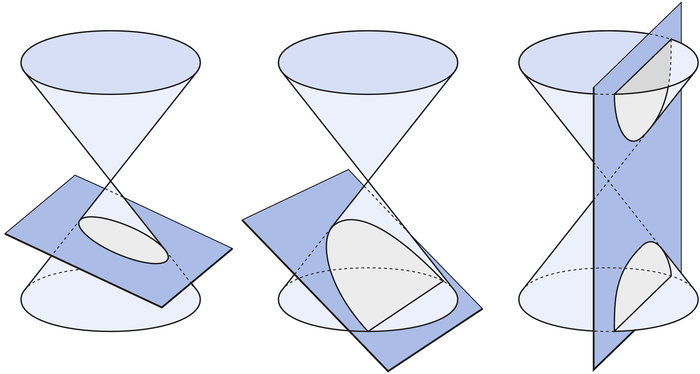
\includegraphics[width=0.6\textwidth]{img/Kegelschnitt.jpg}
\caption{Diverse Kegelschnitte (Grafik: www.duden.de) }
\end{figure} 
\noindent \f{Ziel}: Wir möchten sogenannte ``Kegelschnitte''\index{Kegelschnitte} über $\Zb{R}^2$ mit Hilfe unserer Resultate für Bilinearformen \f{beschreiben}.

\paragraph{Beispiel}
Man beschreibt die ``quadratische Form''
\begin{align}
q(x_1, x_2) = 5 x_{1}^{2} - 2x_1 x_2 + 5x_{2}^{2}
\end{align}
durch eine \f{symmetrische Matrix}
\begin{align}
\begin{pmatrix} 5 & -1 \\ -1 & 5\end{pmatrix}
\end{align}
d.h. 
\begin{align}
q(x_1, x_2) = x^t A x \left( x = \begin{pmatrix} x_1 \\ x_2 \end{pmatrix}\right)
\end{align}
Die Lösungsmenge der quadratischen Gleichung 
\begin{align}
q(x_1, x_2) = 4
\end{align}
ist ein Kegelschnitt, nämlich eine Ellipse. \\\\
\f{Frage:} Wie erkennt man die \f{Form}\footnote{Ellipse, Hyperbel, Parabel} eines Kegelschnitts?\\
Ein \f{Kegelschnitt}\index{Kegelschnitte} ist die Lösungsmenge über $\Zb{R}^2$ einer quadratischen Gleichung der Form:
\begin{align}
\alpha_{11} x_{1}^{2} + 2 \alpha_{12} x_1 x_2 + \alpha_{22} x_{2}^{2} + \beta_1 x_1 + \beta_2 x_2 + \gamma = 0
\end{align}
Der Anteil dieses Kegelschnitts
\begin{align}
q(x_1, x_2) = \alpha_{11} x_{1}^{2} + 2 \alpha_{12} x_1 x_2 + \alpha_{22} x_{2}^{2}
\end{align}
\f{quadratische Form}\index{Form!quadratische}. \\
Man schreibt in Matrixnotation
\begin{align}
x^t A x + Bx + \gamma = 0 \\
\text{mit } x = \begin{pmatrix} x_1 \\ x_2 \end{pmatrix}, A = \begin{pmatrix} \alpha_{11} & \alpha_{12} \\ \alpha_{12} & \alpha_{22} \end{pmatrix}, B = \begin{pmatrix} \beta_1 & \beta_2\end{pmatrix}
\end{align}
\vspace*{0.2cm} \\ \rule{\linewidth}{0.3mm}\vspace*{0.1cm}
\f{Zur Erinnerung} (Satz \ref{satz323}) \\
Jede \f{euklidische Bewegung} $f: \Zb{R}^n \rightarrow \Zb{R}^n$ (eine ``abstandstreue'' Abbildung) ist die Zusammensetzung eines orthogonalen Endomorphismus und einer Translation, d.h. 
\begin{align}
f(x) = Ax + b
\end{align}
für ein $A \in O(n; \Zb{R})$ und $b \in \Zb{R}^n$ \\\\
Wir zeigen, dass \f{entweder}
\begin{align} 
\fbox{$x^t A x + B x + \gamma = 0$} 
\end{align}
einen \f{entarteten} Kegelschnitt beschreibt, d.h. ein Paar von Geraden, eine Gerade, ein Punkt, oder die leere Menge, 
\f{oder} es eine \f{euklidische Bewegung} 
\begin{align}
f: \Zb{R}^2 \rightarrow \Zb{R}^2 
\end{align}
gibt, so dass
\begin{align}
f(x)^t A f(x) + B f(x) + \gamma = 0
\end{align}
eine der folgenden Typen hat:
\begin{itemize}
\item[(i)] \f{Ellipse} 
\begin{align}
\lambda y_{1}^{2} + \mu y_{2}^{2} -1 = 0\, (\lambda, \mu > 0) 
\end{align}

\item[(ii)] \f{Hyperbel}
\begin{align}
\lambda y_{1}^{2} - \mu y_{2}^{2} -1 = 0\, (\lambda, \mu > 0) 
\end{align}

\item[(iii)] \f{Parabel}
\begin{align}
\lambda y_{1}^{2} - y_{2} = 0\, (\lambda > 0) 
\end{align}
\end{itemize}
Man braucht zuerst eine \f{orthogonale} Koordinatentransformation (Drehung, Spiegelung usw.) und eine \f{Translation}.

\paragraph{Beispiel}
Betrachte
\begin{align}
5x_{1}^{2} - 2x_1 x_2 + 5 x_{2}^{2} - 4 = 0 \\
x^t Ax -4 = 0 \\
\text{mit } A = \begin{pmatrix} 5 & -1 \\ -1 & 5 \end{pmatrix}
\end{align}
Man erhält
\begin{align}
p_A(t) = (t-6)(t-4) \\
Eig(A; 6) = Span\{\frac{1}{\sqrt{2}} \begin{pmatrix} 1 \\ -1 \end{pmatrix}\} \\
Eig(A; 4) = Span\{\frac{1}{\sqrt{2}} \begin{pmatrix} 1 \\ 1 \end{pmatrix}\}
\end{align}
Also
\begin{align}
P^t AP = \begin{pmatrix} 6 & 0 \\ 0 & 4 \end{pmatrix}
\end{align}
mit
\begin{align}
P = \frac{1}{\sqrt{2}} \begin{pmatrix} 1 & 1 \\ -1 & 1 \end{pmatrix}
\end{align}
Man setzt
\begin{align}
y = P^t x\, (P^t \text{ orthogonal})
\end{align}
und erhält
\begin{align}
x = Py \\
(Py)^t A (Py) -4 = 0 \\
y^t (P^t AP)y -4 = 0
\end{align}
das heisst
\begin{align}
6y_{1}^{2} + 4 y_{2}^{2} -4 = 0 \\
\text{oder } \frac{3}{2} y_{1}^{2} + y_{2}^{2} -1 = 0 \\
\Rightarrow \text{Ellipse}
\end{align}
Betrachte nun
\begin{align}
x^t Ax + Bx -4 = 0 \\
\text{mit } B = \begin{pmatrix} -\sqrt{2} & \sqrt{2} \end{pmatrix}
\end{align}
Man erhält
\begin{align}
y^t(P^t A P)y + B Py - 4 = 0
\end{align}
das heisst
\begin{align}
6y_{1}^{2} + 4 y_{2}^{2} - 2 y_{1} - 4 = 0
\end{align}
Man setzt
\begin{align}
z = y + \begin{pmatrix} -\frac{1}{6} \\ 0 \end{pmatrix}
\end{align}
und erhält
\begin{align}
6(z_1 + \frac{1}{6}) + 4z_{2}^{2} - 2(z_{1} + \frac{1}{6}) -4 \\
= 6z_{1}^{2} 1 4z_{2}^{2} - \frac{25}{6} = 0 \\
\text{d.h. } \frac{36}{25} z_{1}^{2} + \frac{24}{25} z_{2}^{2} -1 = 0 \\
\Rightarrow \text{Ellipse}
\end{align}
Wir untersuchen nun die allgemeine Gleichung
\begin{align}
x^t Ax + Bx + \gamma = 0 \\
\text{mit } A = \begin{pmatrix} \alpha_{11} & \alpha_{12} \\ \alpha_{12} & \alpha_{22} \end{pmatrix}, B = \begin{pmatrix} \beta_1, \beta_2 \end{pmatrix}
\end{align}
Nach dem \f{Spektralsatz} (\ref{satz556}) gibt es eine \f{orthogonale} Matrix $P \in Mat(2; \Zb{R})$. sp dass $P^t A P$ diagonal ist. Man setzt
\begin{align}
y = P^t x
\end{align}
und erhält
\begin{align}
(Py)^t A (Py) + B(Py) + \gamma = 0 \\
y^t (\underbrace{P^t A P}_{Diag.-Mat.}) y + (BP)y + \gamma = 0
\end{align}
Also nehmen wir jetzt an, dass A \f{diagonal} ist, d.h.
\begin{align}
\alpha_{11} x_{1}^{2} + \alpha_{22} x_{2}^{2} + \beta_1 x_1 + \beta_2 x_2 + \gamma = 0
\end{align}
Wenn $\alpha_{11} \neq 0, \alpha_{22} \neq 0$, setzt man für $i = 1, 2:$
\begin{align}
z_i = x_i + \frac{\beta_i}{2 \alpha_{ii}}
\end{align}
und erhält für ein $\gamma' \in \Zb{R}$
\begin{align}
\alpha_{11} z_{1}^{2} + \alpha_{22} z_{2}^{2} - \gamma' = 0
\end{align}
Ist $\gamma' = 0$, so definiert die Gleichung ein Paar von Geraden oder einen Punkt, d.h. der Kegelschnitt ist \f{entartet}. \\
Ist $\gamma' \neq 0$,, erhält man
\begin{align}
\frac{\alpha_{11} z_{1}^{2}}{\gamma'} + \frac{\alpha_{22} z_{2}^{2}}{\gamma'} - 1 = 0 \\
-z_{1}^{2} - z_{2}^{2} -1 = 0
\end{align}
Wenn $\frac{\alpha_{11}}{\gamma'}, \frac{\alpha_{22}}{\gamma'} < 0$, dann ist der Kegelschnitt \f{leer} und entartet.
Für $\frac{\alpha_{11}}{\gamma'}, \frac{\alpha_{22}}{\gamma'} > 0$ erhält man eine \f{Ellipse}, andernfalls eine \f{Hyperbel}. \\
Falls $\alpha_{22} = 0, \beta_2 \neq 0, \alpha_{11} \neq 0$ definiert man
\begin{align}
z_1 = x_1 + \frac{\beta_1}{2 \alpha_{11}} \\
z_2 = x_2 + \frac{\gamma + \frac{\beta_{1}^{2}}{4 \alpha_{11}^{2}}}{\beta_{2}}
\end{align}
und erhält
\begin{align}
\alpha_{11} z_{1}^{2} + \beta_{2} z_{2} = 0
\end{align}
und dann
\begin{align}
- \frac{\alpha_{11}}{\beta_2} z_{1}^{2} - z_2 = 0
\end{align}
Schliesslich kann man, falls $\frac{-\alpha_{11}}{\beta_1} < 0$ durch eine Spiegelung das Vorzeichen ändern. Man erhält eine \f{Parabel}. \\\\
Der Fall $\alpha_{11} = 0, \beta_1 \neq 0, \alpha_{22} \neq 0$ ist sehr ähnlich. Die übrigen Fälle definieren entartete Kegelschnitte (Aufgabe).

%DATE 18.05.2012
\newpage
\noindent \textit{Vorlesung vom 18.05.2012} \\\\
%\Large \f{???} \normalsize \\\\
\f{Beispiele} 
\begin{itemize}
\item[(i)] Betrachte
\begin{align}
x^t Ax - 6 = 0
\end{align}
mit 
\begin{align}
A = \begin{pmatrix} 1 & -2 \\ -2 & 3\end{pmatrix}
\end{align}
d.h.
\begin{align}
x_1^2 - 4x_1 x_2 + 3x_2^2 - 6 = 0
\end{align}
Man erhält:
\begin{align}
p_A(t) &= \begin{pmatrix} t-1 & 2 \\ 2 & t-3 \end{pmatrix} \\
 &= (t-1)(t-3)-4 \\
 &= t^2 - 4t -1 \\
 &= (t - (2+ \sqrt{5})) (t-(2- \sqrt{5})) 
\end{align}
\begin{align}
Eig(A, 2 + \sqrt{5}): \\
= Span\left\{ \frac{1}{\sqrt{10-2\sqrt{5}}} \begin{pmatrix} 1 - \sqrt{5} \\ 2 \end{pmatrix} \right\}
\end{align}
\begin{align}
Eig(A, 2 - \sqrt{5}): \\
= Span\left\{ \frac{1}{\sqrt{10-2\sqrt{5}}} \begin{pmatrix} 2 \\ 1 - \sqrt{5} \end{pmatrix} \right\}
\end{align}
Also
\begin{align}
 P^t A P = \begin{pmatrix} 2 + \sqrt{5} & 0 \\ 0 & 2-\sqrt{5}\end{pmatrix}
\end{align}
mit
\begin{align}
P = \frac{1}{\sqrt{10-2\sqrt{5}}} \begin{pmatrix} 1- \sqrt{5} & 2 \\ 2 & -1+ \sqrt{5} \end{pmatrix}
\end{align}
Man erhält für $y = P^t x$:
\begin{align}
(2 + \sqrt{5})y_1^2 + (2 - \sqrt{5})y_2^2 - 6 &= 0 \\
\frac{2 + \sqrt{5}}{6} y_1^2 + \frac{2 - \sqrt{5}}{6} y_2^2 - 1 &= 0 \\
\end{align}
den Kegelschnitt einer \f{Hyperbel}\index{Hyperbel}.

\item[(ii)] Betrachte
\begin{align}
x^t Ax - 4 = 0 \text{ mit } A = \begin{pmatrix} -5 & 1 \\ 1 & -5\end{pmatrix}
\end{align}
Man erhält (siehe oben) 
\begin{align}
P^t A P = \begin{pmatrix} -6 & 0 \\ 0 & -4 \end{pmatrix} \text{ mit } P = \frac{1}{\sqrt{2}} \begin{pmatrix} 1 & 1 \\ -1 & 1 \end{pmatrix}
\end{align}
Man setzt $y = P^t x$ und erhält:
\begin{align}
-6y_1^2 - 4y_2^2 - 4 = 0 \\
6y_1^2 + 4y_2^2 + 4 = 0
\end{align}
\f{entartet}.\\\\
Betrachte nun
\begin{align}
x^t Ax + Bx -4 = 0 \text{ mit } A = \begin{pmatrix} -5 & 1 \\ 1 & -5\end{pmatrix}, B = \begin{pmatrix} 12 & -12\end{pmatrix}
\end{align}
Man erhält für $< = P^t x$
\begin{align}
-6y_1^2 + 4y_2^2 + 12 \sqrt{2} y_1 - 4 = 0
\end{align}
und dann für
\begin{align}
z_1 &= y_1 + \frac{12\sqrt{2}}{-6 \cdot 2} = y_1 - \sqrt{2} \\
z_2 &= y_2
\end{align}
\begin{align}
-6(z_1 + \sqrt{2})^2 + 4z_2^2 + 12 \sqrt{2} (z_1 + \sqrt{2}) - 4 &= 0 \\
-6z_1^2 - 4z_2^2 + 8 &= 0
\end{align}
d.h. eine \f{Ellipse}.
\begin{align}
\frac{3z_1^2}{2} + \frac{1}{2}z_2^2 -1 = 0
\end{align}
\end{itemize}
Eine \f{Quadrik}\index{Quadrik} ist die Lösungsmenge über $\Zb{R}^n$ einer quadratischen Gleichung der Form
\begin{align}
\sum_{i=1}^{n} \alpha_{ii} x_i^2 + \sum_{1 \leq i, j \leq n}^{n} 2 \alpha_{ij} x_i x_j + \sum_{i=1}^{n} \beta_i x^i + y = 0
\end{align}
oder in Matrixform:
\begin{align}
&x^t A x + Bx + \gamma = 0 \\ 
\text{ mit } A &= \begin{pmatrix} \alpha_{11} & \alpha_{12} & \cdots & \alpha_{1n} \\ \alpha_{12} & \ddots & \ddots & \vdots \\ \vdots & \ddots & \ddots & \vdots \\ \alpha_{1n} & \cdots & \cdots & \alpha_{nn}\end{pmatrix}, B = \begin{pmatrix} \beta_1 & \cdots & \beta_n \end{pmatrix}
\end{align}
Nach einer geeigneten orthogonalen Transfomration $P$ wird die Quadrik durch eine Gleichung 
\begin{align}
y^t (P^t A P) y + B Py + Y = 0
\end{align}
beschrieben, wobei $P^t A P$ \f{diagonal} ist. \\
Durch Translationen eliminiert man die Terme $\beta_i x_i$.
In $\Zb{R}^3$ ist eine Quadrik entweder \f{entartet} oder es gibt eine euklidische Bewegung\index{euklidische Bewegung} $f: \Zb{R}^3 \rightarrow \Zb{R}^3$, so dass
\begin{align}
f(x)^t A f(x) + B f(x) + \gamma = 0
\end{align}
eine der folgenden Typen hat:
\begin{itemize}
\item[(i)] \f{Ellipsoide}\index{Ellipsoid}: $\alpha_{11} x_1^2 + \alpha_{22} x_2^2 + \alpha_{33} x_3^2 -1 = 0$
\item[(ii)] \f{Einschalige Hyperboloide}\index{Hyperboloid}: $\alpha_{11} x_1^2 + \alpha_{22} x_2^2 - \alpha_{33} x_3^2 -1 = 0$
\item[(iii)] \f{Zweischalige Hyperboloide}: $\alpha_{11} x_1^2 - \alpha_{22} x_2^2 - \alpha_{33} x_3^2 -1 = 0$
\item[(iv)] \f{Elliptische Paraboloide}\index{Paraboloid}: $\alpha_{11} x_1^2 + \alpha_{22} x_2^2 - x_3 -1 = 0$
\item[(v)] \f{Hyperbolische Paraboloide}: $\alpha_{11} x_1^2 - \alpha_{22} x_2^2 - x_3 -1 = 0$
\end{itemize}
wobei $\alpha_{11}, \alpha_{22}, \alpha_{33} > 0$ sind.

\paragraph{Beispiel}
\begin{align}
5x_1^2 + 5x_2^2 + 2x_3^2 + 8x_1 x_2 + 4x_1 x_3 + 4x_2 x_3 + x_1 - 2x_3 -1 = 0 \\
x^t A x + Bx -1 = 0 \text{ mit } A = \begin{pmatrix}5 & 4 & 2 \\ 4 & 5 & 2 \\ 2 & 2 & 2 \end{pmatrix}, B = \begin{pmatrix} 1 & 0 & -2\end{pmatrix}
\end{align}
Dann (siehe oben)
\begin{align}
P^t A P = \begin{pmatrix} 1 & 0 & 0 \\ 0 & 1 & 0 \\ 0 & 0 & 10 \end{pmatrix} \text{ mit } P = \frac{1}{\sqrt{5}} \begin{pmatrix} 1 & -\frac{4}{3} & 2 \\ 0 & \frac{5}{3} & 2 \\ -2 & -\frac{2}{3} & 1 \end{pmatrix}
\end{align}
Man erhält für $y = P^t x$
\begin{align}
y_1^2 y_2^2 + y_3^2 + \sqrt{5} y_1 -1 = 0
\end{align}
und dann gilt für 
\begin{align}
z_1 = y_1 + \frac{\sqrt{5}}{2}. z_2 = y_2, z_3 = y_3 \\
z_1^2 + z_2^2 + 10z_3^2 - \frac{9}{4} = 0 
\end{align}
oder 
\begin{align}
\frac{4}{9}z_1^2 + \frac{4}{9} z_2^2 + \frac{40}{9} z_3^2 -1 = 0
\end{align}
$\rightarrow$ \f{Ellipsoid}.

\paragraph{Bemerkung}
Man kann oft den Typ einer Quadrik ohne komplizierte Berechnungen bestimmen.\\
\f{Beispiel}: Für einen \f{nicht entarteten} Kegelschnitt, beschrieben durch
\begin{align}
x^t Ax + Bx + \gamma = 0
\end{align}
erhält man 
\begin{itemize}
\item eine \f{Ellipse}\index{Ellipse} gdw. $det\, A > 0$
\item eine \f{Hyperbel}\index{Hyperbel} gdw. $det\, A < 0$
\item eine \f{Parabel}\index{Parabel} gdw. $det\, A = 0$ 
\end{itemize}
Zudem kann mit Koordinatenwechsel evtl. nicht orthogonal bestimmt werden, ob ein Kegelschnitt entartet ist.

\section{Der Spektralsatz für normale Endomorphismen}
Zur Erinnerung: Für jede hermitesche Matrix $A \in Mat(n; \Zb{C}), (A = A^{*})$ gibt es eine unitäre Matrix $P$, so dass $P^{*} A P$ diagonal ist.
\paragraph{Frage:} Welche (anderen) Matrizen haben diese Eigenschaft? \\
Eine Matrix $A \in Mat(n; \Zb{C})$ heisst \f{normal}\index{normal}, wenn $A$ und $A^{*}$ vertauschbar sind, d.h. $A^{*} A = A A^{*}$.

\paragraph{Bemerkung}
Jede \f{hermitesche} Matrix\index{Matrizen!hermitesch} $A \in Mat(n; \Zb{C})$ ist normal.
\begin{align}
A A^{*} = A^2 = A^{*} A
\end{align}
auch jede \f{schiefsymmetrische Matrix}\index{Matrizen!schiefsymmetrisch} ($A^{*} = - A$)
\begin{align}
A A^{*} = - A^2 = A^{*} A
\end{align}
und jede \f{unitäre Matrix}\index{Matrizen!unitär}
\begin{align}
A A^{*} =  E = A^{*} A
\end{align}
Es gibt auch andere Beispiele, z.B.
\begin{align}
A = \begin{pmatrix} 1 & 1 & 0 \\ 0 & 1 & 1 \\ 1 & 0 & 1 \end{pmatrix}, A A^{*} = A^{*} A = \begin{pmatrix} 2 & 1 & 1 \\ 1 & 2 & 1 \\ 1 & 1 & 2\end{pmatrix}
\end{align}

\begin{lemma} % 5.7.1
\label{lemma571}
Sei $P \in Mat(n; \Zb{C})$ unitär. Dann ist $A \in Mat(n; \Zb{C})$ normal gdw. $P^{*} A P^{*}$ normal ist
\end{lemma}
\paragraph{Beweis}
\begin{itemize}
\item[``$\Rightarrow$''] $A \leftarrow Mat(n; \Zb{C})$ unitär.
\begin{align}
&\Rightarrow AA^{*} = A^{*} A \\
&\Rightarrow (P^{*} A P) (P^{*} A P)^{*} \\
&= (P^{*} A P) (P^{*} A^{*} P) \\
&= P^{*} A A^{*} P\\
&= P^{*} A^{*} P = (P^{*} A P)^{*} (P^{*} A P)
\end{align}

\item[``$\Leftarrow$''] $P^{*} A P$ normal.
\begin{align}
&\Rightarrow P^{**} P^{*} A P^{*} P^{*} \text{ ist normal (nach ``$\Rightarrow$'')} \\
&\Rightarrow A \text{ ist normal}
\end{align}
\end{itemize}
\hfill $\Box$ \\\\
Ein Endomorphismus $f: V \rightarrow V$ eines \f{hermiteschen Raumes} $V$ (endlich-dimensional über $\Zb{C}$ mit einer positiv definiten hermiteschen Form) heisst \f{normal}\index{normal}, wenn die zugehörige Matrix bezüglich einer (und damit jeder) Orthonormalbasis normal ist. \\\\

\begin{satz} % 5.7.2
\label{satz572} %{\ \\}
$A \in Mat(n; \Zb{C})$ ist normal gdw. es ein unitäre Matrix $P \in Mat(n; \Zb{C})$ gibt, so dass $P^{*} A P$ diagonal ist.
\end{satz}

\paragraph{Beweis}
\begin{itemize}
\item[``$\Rightarrow$''] Jede \f{Diagonalmatrix} ist normal. Also ist $P^{*} A P^{*}$ diagonal, dann ist $A$ nach Lemma \ref{lemma571} auch normal.

\item[``$\Leftarrow$''] Sei $A \in Mat(n; \Zb{C})$ \f{normal}. Man wählt einen Eigenvektor $v= v$, und normiert ihn auf Länge 1, so dass $<v, v> = 1$ gilt. \\
Dann ergänzt man $(v_1)$ zu einer Orthonormalbasis von $\Zb{C}^n$. Man erhält ein unitäres $P \in Mat(n; \Zb{C})$ und $B \in Mat(n-1; \Zb{C})$, so dass
\begin{align}
P^{*} A P &= \begin{pmatrix}[c|ccc] \alpha_{11} & \alpha_{12} & \cdots & \alpha_{1n} \\ 0 & & & \\ \vdots & & B & \\ 0 & & & \end{pmatrix} \text{ und} \\
(P^{*} A P)^{*} &= \begin{pmatrix}[c|ccc] \overline{\alpha_{11}} & 0 & \cdots & 0 \\ \overline{\alpha_{12}} & & & \\ \vdots & & B^{*} & \\ \overline{\alpha_{1n}} & & & \end{pmatrix}
\end{align}
\end{itemize}
\hfill $\Box$ \\\\
$P^{*} A P$ ist \f{normal} (Lemma \ref{lemma571}) und deshalb sind die oberen linken Einträge von $(P^{*} A P) (P^{*} A P)^{*}$ und $(P^{*} A P)^{*}(P^{*} A P)$
\f{gleich} das heisst
\begin{align}
\alpha_{11} \overline{\alpha_{11}} = \alpha_{11} \overline{\alpha_{11}} + \alpha_{12} \overline{\alpha_{12}} + ... + \alpha_{1n} \overline{\alpha_{1n}}
\end{align}
Daraus folgt
\begin{align}
\alpha_{12} \overline{\alpha_{12}} + ... + \alpha_{1n} \overline{\alpha_{1n}} = 0
\end{align}
und (da $\alpha_{1i} \overline{\alpha_{1i}} \in \Zb{R}$ und $\geq 0$)
\begin{align}
\alpha_{12} = \alpha_{13} = ... =  \alpha_{1n} = 0
\end{align}
d.h.
\begin{align}
P^{*} A P = \begin{pmatrix}[c|ccc] \alpha_{11} & 0 & \cdots & 0 \\ 0 & & & \\ \vdots & & B & \\ 0 & & & \end{pmatrix}
\end{align}
$B$ ist auch normal und die Behauptung folgt durch Induktion nach $n$.
\hfill $\Box$

\paragraph{Beispiel}
\begin{align}
A = \begin{pmatrix} 3 & 2 \\ -2 & 3 \end{pmatrix}
\end{align}
ist normal.
\begin{align}
det(t E - A) &= \begin{vmatrix} t-3 & -2 \\ 2 & t-3 \end{vmatrix} \\
&= (t-3)^2 + 4 \\
&= (t - (3 + 2i)) (t - (3 - 2i))
\end{align}
Eigenwerte: $3 + 2i, 3-2i$.
\begin{align}
Eig(A; 3 + 2i) = Span\{\frac{1}{\sqrt{2}} \begin{pmatrix} 1 \\ i\end{pmatrix}\} \\
Eig(A; 3 - 2i) = Span\{\frac{1}{\sqrt{2}} \begin{pmatrix} 1 \\ -i\end{pmatrix}\} \\
P^{*} A P = \begin{pmatrix} 3 + 2i & 0 \\ 0 & 3-2i \end{pmatrix} \text{ mit } P = \frac{1}{\sqrt{2}}\begin{pmatrix} 1 & 1 \\ i & -i\end{pmatrix} \text{ \f{unitär}}
\end{align}

\begin{korollar} % 5.7.3
\label{korollar573}
Jede konjugierte Klasse in der unitären Gruppe enthält eine Diagonalmatrix, dass heisst für eine unitäre Matrix $P \in Mat(n; \Zb{C})$ existiert $Q$ unitär, so dass $Q^{*} P Q$ \f{unitär} und \f{diagonal} ist.
\end{korollar}
\paragraph{Beispiel}
\begin{align}
P = \frac{1}{\sqrt{2}} \begin{pmatrix} 1 & i \\ i & 1\end{pmatrix} \text{ ist unitär}
\end{align}
Man erhält
\begin{align}
Q^{*} P Q = \frac{1}{\sqrt{2}} \begin{pmatrix} 1+i & 0 \\ 0 & 1-i\end{pmatrix} 
\end{align}
unitär mit
\begin{align}
Q = \frac{1}{\sqrt{2}} \begin{pmatrix} 1 & 1 \\ 1 & -1 \end{pmatrix}
\end{align}

%DATE 21.05.2012
\newpage
\noindent \textit{Vorlesung vom 21.05.2012} 
\section{Andere Darstellungen} % 5.8
\paragraph{Alternierende und schiefsymmetrische Bilinearformen} {\ \\}
Eine Bilinearform $<, >$ auf einem Vektorraum über $V$ heisst \f{alternierend}\index{alternierend}, wenn $\forall v \in V$ gilt:
\begin{align}
<v, v> = 0
\end{align}
Daraus folgt, dass $\forall v, w \in V$ gilt:
\begin{align}
0 = <v+w, v+w> &= <v, v> + <v, w> + <w, v> + <w, w> \\
&= <v, w> + <w, v>
\end{align}
und deshalb
\begin{align}
<v, w> = - <w, v>
\end{align}
d.h. $<, >$ ist schiefsymmetrisch.\\\\
Ist $1+1 \neq 0$ in $K$m dann gilt auch die andere Richtung:
\begin{align}
<,> \text{ ist schiefsymmetrisch } &\Rightarrow \forall v \in V: <v, v> = -<v, v> \\
&\Rightarrow (1+1) <v, v> = 0 \\
&\Rightarrow <v, v> = 0
\end{align}
d.h. $<, >$ ist alternierend.\\\\
Eine Matrix
\begin{align}
A = (\alpha_{ij}) \in Mat(n;K)
\end{align}
von einer alternierenden Bilinearform $<, >$ bezüglich einer Basis auf einem endlich-dimensionalen Vektorraum $V$ über $K$ hat die Eigenschaft
\begin{align}
\alpha_{ij} = \left\{\begin{matrix} -\alpha_{ji} & \text{ wenn } i \neq j \\ 0 & \text{ wenn } i = j \end{matrix} \right.
\end{align}
und deshalb auch
\begin{align}
A^t = -A
\end{align}
d.h. $A$ ist schiefsymmetrisch.\\\\
Wenn $1+1 \neq 0$ und $A^t = -A$, dann hat $A$ auch diese Eigenschaft, aber für $1+1 \neq 0$ gilt diese Richtung nicht. Zum Beispiel:
\begin{align}
\begin{pmatrix} 1 & 1 \\ 1 & 1\end{pmatrix}^t = - \begin{pmatrix}1 & 1 \\ 1 & 1\end{pmatrix}
\end{align}
Jede reelle schiefsymmetrische Matrix $A \in Mat(n; \Zb{R})$ ist \f{normal}, also
\begin{align}
A A^{*} = A A^{t} = -A^{2} = A^{t} A = A^{*} A
\end{align}
und deshalb nach dem Spektralsatz unitär diagonalisierbar über $\Zb{R}$.\\
Beispiel:
\begin{align}
A = \begin{pmatrix} 0 & 1 \\ -1 & 0 \end{pmatrix} \in Mat(2; \Zb{R}) \\
P^{-1} A P = \begin{pmatrix} 1 & 0 \\ 0 & -1 \end{pmatrix} \text{ mit } P = \frac{1}{\sqrt{2}} \begin{pmatrix}i & i \\ -1 & 1\end{pmatrix}
\end{align}
Beachte nun, dass wenn $A \in Mat(n; \Zb{C})$ schiefsymetrisch ist und $1+1 \neq 0 \in K$, gilt:
\begin{align}
A \text{ invertierbar } \Rightarrow n \text{ gerade} \\
(det\, A \neq 0)
\end{align}

\begin{align}
n \text{ ungerade } \Rightarrow det\, A &= det(-A^t) \\
&= det(-A) \\
&= (-1)^n det\, A \\
&= -det\, A \\
\Rightarrow (1+1)\, det\, A &= 0 \\
\Rightarrow det\, A &= 0
\end{align}
Beachte auch, dass
\begin{align}
A \text{ invertierbar und schiefsymmetrisch} \Rightarrow (A^{-1})^t = (A^t)^{-1} \\
= -A^{-1} \text{ (d.h. $A^{-1}$ schiefsymmetrisch)}
\end{align}

\begin{satz} % 5.8.1
\label{satz581}
\begin{itemize}
\item[(a)] Sei $V$ ein Vektorraum der Dimension $n$ über $K$, und sei $<, >$ eine nicht-entartete alternierende Bilinearform auf $V$. Dann ist $n$ eine gerade Zahl, und es gibt eine Basis von $V$ bezüglich der die Matrix von $<, >$ die folgende Form hat:
\begin{align}
J_{2m} = \begin{pmatrix}0m & Em \\ -Em & 0m\end{pmatrix} \text{ mit } m = \frac{n}{2}
\end{align}

\item[(b)] Sei $A \in Mat(n; \Zb{C})$ invertierbar und alternierend. Dann ist $n$ gerade und es gibt ein invertierbares Produkt $P \in Mat(n; K)$ so dass $P^{t} A P = J_{2m}$ mit $m = \frac{n}{2}$.
\end{itemize}
\end{satz}

\paragraph{Beweis}
Man zeigt:
\begin{itemize}
\item $<, >$ ist nicht-entartet gdw. eine zugehörige Matrix bezüglich einer Basis invertierbar ist.
\item $V = W \oplus W^{\perp}$, wenn $<, >$ auf einem Unterraum $W$ von $V$ nicht-entartet ist.
\item Wenn $<, >$ nicht identisch Null ist, dann gibt es einen Unterraum $W$, so dass $<, >$ auf $W$ bezüglich einer geeigneten Basis durch die Matrix
\begin{align}
\begin{pmatrix} 0 & 1 \\ -1 & 1\end{pmatrix}
\end{align}
beschrieben ist.
\end{itemize}

\paragraph{Bemerkung}
Ein Vektorraum mit einer nicht-entarteten alternierenden Bilinearform heisst \f{symplektrischer}\index{symplektisch} Raum.

% Index / Stichwortverzeichnis
\printindex

\end{document}
